%!TEX encoding = UTF-8 Unicode

\documentclass[a4paper,11pt,obeyspaces,openany]{book}
% L'option 'openany' permet de démarrer un chapitre sur une page paire

% L'option 'obeyspaces' indique au paquetage hyperref de respecter les espaces dans les chemins \path ou \url.
%
% Par exemple : \path{ab cd} est écrit ab cd
% Sans cette option, \path{ab cd} est écrit abcd
% Voir : http://compgroups.net/comp.text.tex/space-in-path-hyperref-package

%-----------------------------------------------------------------------------------------------------------------------*
%                                                                                                                       *
%   « N O I R    E T    B L A N C »    O U    « C O U L E U R »                                                         *
%                                                                                                                       *
%-----------------------------------------------------------------------------------------------------------------------*

%--- Par défaut, l'impression se fait en couleur
\providecommand{\sortieEnCouleur}{true}

%-----------------------------------------------------------------------------------------------------------------------*
%                                                                                                                       *
%   A F F I C H E R    L E    D E T A I L    D E S    S C H É M A S    É L E C T R O N I Q U E S                        *
%                                                                                                                       *
%-----------------------------------------------------------------------------------------------------------------------*

%--- Par défaut, le détail des schémas est affiché
\providecommand\afficherDetailSchema{true}

%-----------------------------------------------------------------------------------------------------------------------*
%                                                                                                                       *
%   E N C O D A G E    D E S    S O U R C E S     :     U T F 8                                                         *
%                                                                                                                       *
%-----------------------------------------------------------------------------------------------------------------------*

%--- Paquetage pour le codage des sources en UTF-8
\usepackage[utf8]{inputenc}

%--- Latex demande ce paquetage pour mieux afficher le caractère "°" et \textquotesingle "'"
\usepackage{textcomp}

%--- Ce paquetage permet d'effectuer certaines césures, et ainsi d'éviter les messages "Overfull \hbox"
\usepackage[T1]{fontenc}

\usepackage{lmodern} % for French

%-----------------------------------------------------------------------------------------------------------------------*
%                                                                                                                       *
%   R É G L A G E S    « F R A N Ç A I S »                                                                              *
%                                                                                                                       *
%-----------------------------------------------------------------------------------------------------------------------*

%--- Paquetage pour imposer les réglages français
%\usepackage[francais]{babel}
\usepackage[frenchb]{babel}

%--- Contrôle de l'indentation et de la séparation des paragraphes
\setlength{\parindent}{0pt} 
%\setlength{\parskip}{1.2ex} % Reporté avant les chapitres

%--- Ajouter une séparation à la fin des itemize
\let\EndItemize\enditemize
\def\enditemize{\EndItemize\vspace{1.2ex}}

%-----------------------------------------------------------------------------------------------------------------------*
%                                                                                                                       *
%   M I S E    E N    P A G E S    D E M A N D É E     P A R     E L L I P S E S                                        *
%                                                                                                                       *
%-----------------------------------------------------------------------------------------------------------------------*

%---------------------------------------------------- Mise en page
% Voir "Une courte introduction à Latex2e", § 6.4

%--- Marge gauche : 2,8 cm ; le paramètre \hoffset contient cette valeur, moins 1 pouce
%    \hoffset = 2,8 cm - 2,54 cm = 0,26 cm
\setlength{\hoffset}{-0.26 cm}
%
%%--- Hauteur de la page : 29,7 cm
%\setlength{\paperheight}{29.7 cm}
%
%--- Largeur de la page
%\setlength{\paperwidth}{18 cm}
%
%%--- Marges supplémentaires, différenciées pour les pages gauches et droites ; ici, aucune.
%\setlength{\oddsidemargin }{0 cm}
%\setlength{\evensidemargin}{0 cm}
%
%--- Largeur du texte
\setlength{\textwidth}{14 cm}
%
%%--- Marge haute : 2,8 cm ; le paramètre \voffset contient cette valeur, moins 1 pouce
%%    \voffset = 2,8 cm - 2,54 cm = 0,26 cm
%\setlength{\voffset}{0.26 cm}
%
%%--- Distance entre la marge haute et l'en-tête : 0 cm
%\setlength{\topmargin}{0 cm}
%
%%--- Hauteur de l'en-tête de chaque page : 1 cm
%\setlength{\headheight}{1 cm}
%
%%--- Distance entre l'en-tête de chaque page et le corps : 0,5 cm
%\setlength{\headsep}{0.5 cm}
%
%%--- Hauteur du corps
%%    \textheight = 29,7 cm - 2,8 cm - 2,8 cm - 1,5 cm = 22,6 cm
%\setlength{\textheight}{22.6 cm}
%
%%--------------------- Changer la taille des notes en bas de page
%%  footnotesize ---> small
%
%\let\oldfootnotesize\footnotesize
%\renewcommand*{\footnotesize}{\oldfootnotesize\small}

%-----------------------------------------------------------------------------------------------------------------------*
%                                                                                                                       *
%   P A Q U E T A G E    « I F T H E N »                                                                                *
%                                                                                                                       *
%-----------------------------------------------------------------------------------------------------------------------*

%--- Ce paquetage permet d'effectuer des tests : \ifthenelse{test}{bloc then}{bloc else}
\usepackage{ifthen}

%-----------------------------------------------------------------------------------------------------------------------*
%                                                                                                                       *
%   G E S T I O N    D E    L ' I N D E X                                                                               *
%                                                                                                                       *
%-----------------------------------------------------------------------------------------------------------------------*

% http://www.cuk.ch/articles/4097
% http://www.tuteurs.ens.fr/logiciels/latex/makeindex.html
% http://linux.die.net/man/1/makeindex
%
% Attention ! Les deux commandes suivantes, ainsi que le \printindex placé plus bas ne
% sont pas suffisants pour construire l'index : il faut utiliser l'utilitaire "makeIndex"
% Voir le fichier de commande "build.command"
\usepackage{makeidx}
\makeindex

%-----------------------------------------------------------------------------------------------------------------------*
%                                                                                                                       *
%   H Y P E R R E F                                                                                                     *
%                                                                                                                       *
%-----------------------------------------------------------------------------------------------------------------------*


%--- Pour les hyperliens, et le contrôle de la génération PDF 
\usepackage[pagebackref]{hyperref}

\hypersetup{pdftitle      = {Piccolo}}
\hypersetup{pdfauthor     = {Pierre Molinaro}}

\hypersetup{colorlinks    = true}
\hypersetup{anchorcolor   = black}
\hypersetup{filecolor     = black}
\hypersetup{menucolor     = black}
\hypersetup{plainpages    = false}
\hypersetup{pdfstartview  = FitH}
\hypersetup{pdfpagelayout = OneColumn}

%--- Contrôle des références de la bibliographie ; avec ces lignes, les pages où chaque item de la biblio
%    est appelée sont insérées à la fin de chaque entrée.
%\hypersetup{backref        = page}

\renewcommand*{\backrefalt}[4]{
  \ifcase #1 % case: not cited
    \ifthenelse{\equal{\sortieEnCouleur}{true}}{\textcolor{red}{\textbf{(non cité)}}}{\textbf{(non cité)}}. 
  \or % case: cited on exactly one page 
    (cité page #2).% 
  \else % case: cited on multiple pages 
    (cité pages #2). 
  \fi
} 
\renewcommand*{\backreftwosep}{ et }
\renewcommand*{\backreflastsep}{ et }


%--- Les hyperliens sont colorés en bleu dans la phase de mise au point, ils sont ainsi mieux visibles
\ifthenelse{\equal{\sortieEnCouleur}{true}}{
  \hypersetup{linkcolor  = blue}
  \hypersetup{urlcolor   = blue}
  \hypersetup{citecolor  = blue}
}{
  \hypersetup{linkcolor  = black}
  \hypersetup{urlcolor   = black}
  \hypersetup{citecolor  = black}
}

%---------------------------------------------------- Numéro de section
% Par défaut, une section est affichée avec son numéro de chapitre : par exemple : 2.1 Titre
% Les Éditions Ellipses précisent que le numéro de chapitre ne doit pas apparaître, ni dans le corps, ni dans l'en-tête
% Voir http://help-csli.stanford.edu/tex/latex-sections.shtml
% La solution suivante affecte aussi les sous-sections, ainsi que la table des matières.
%\renewcommand\thesection {\arabic{section}}

%---------------------------------------------------- Affichage des numéros de section
% C'est à dire les numéros qui sont affichées pour \section, \subsection, ...
% Par défaut, l'affichage se fait jusqu'au niveau 2 (\subsection)
% Avec cette commande, on va jusqu'au niveau \subsubsection.
%\setcounter{secnumdepth}{3}

%---------------------------------------------------- Définition de subsubsubsection
% http://forum.mathematex.net/latex-f6/definir-un-subsubsubsection-t4031.html
\makeatletter
\newcounter{subsubsubsection}[subsubsection]
\renewcommand\thesubsubsubsection{\thesubsubsection .\@alph\c@subsubsubsection}
\newcommand\subsubsubsection{\@startsection{subsubsubsection}{4}{\z@}%
                                     {-3.25ex\@plus -1ex \@minus -.2ex}%
                                     {1.5ex \@plus .2ex}%
                                     {\normalfont\normalsize\bfseries}}
\newcommand*\l@subsubsubsection{\@dottedtocline{3}{10.0em}{4.1em}}
\newcommand*{\subsubsubsectionmark}[1]{}
\makeatother

\makeatletter
\def\toclevel@subsubsubsection{4}
\makeatother

%------------------------------------------------------------------------------------------ RÉFÉRENCES À UN TABLEAU
% La référence au tableau "nom-du-tableau" est définie par \labelTableau{nom-du-tableau}
\newcommand\labelTableau[1]{\label{tab:#1}}
% Latex autorise deux types d'appel à une référence \ref{tab:nom-du-tableau} et \pageref{tab:nom-du-tableau}

% \refTableau{}{nom-du-tableau} ---> "tableau x.y"   où x.y est le n° du tableau
\newcommand\refTableau[1]{\hyperref[tab:#1]{tableau \ref*{tab:#1}}}

% \refTableauSansPrefixe{}{nom-du-tableau} ---> "x.y"   où x.y est le n° du tableau
\newcommand\refTableauSansPrefixe[1]{\hyperref[tab:#1]{\ref*{tab:#1}}}

% \refTableauPage{}{nom-du-tableau} ---> "tableau x.y page n"   où x.y est le n° du tableau
\newcommand\refTableauPage[1]{\hyperref[tab:#1]{tableau \ref*{tab:#1} page \pageref{tab:#1}}}

% \refTableauPageSansPrefixe{}{nom-du-tableau} ---> "x.y page n"   où x.y est le n° du tableau
\newcommand\refTableauPageSansPrefixe[1]{\hyperref[tab:#1]{\ref*{tab:#1} page \pageref{tab:#1}}}

%------------------------------------------------------------------------------------------ RÉFÉRENCES À UNE FIGURE
% La référence au tableau "nom-de-la-figure" est définie par \labelFigure{nom-de-la-figure}
\newcommand\labelFigure[1]{\label{fig:#1}}
% Latex autorise deux types d'appel à une référence \ref{fig:nom-de-la-figure} et \pageref{fig:nom-de-la-figure}

% \refFigure{}{nom-de-la-figure}   ---> "figure x.y"   où x.y est le n° de la figure
% \refFigure{z}{nom-de-la-figure}  ---> "figure x.y.z" où x.y est le n° de la figure
\newcommand\refFigure[2]{\hyperref[fig:#2]{figure \ref*{fig:#2}{\ifthenelse{\equal{#1}{}}{}{.#1}}}}

% \refFigureSansPrefixe{}{nom-de-la-figure}   ---> "x.y"   où x.y est le n° de la figure
% \refFigureSansPrefixe{z}{nom-de-la-figure}  ---> "x.y.z" où x.y est le n° de la figure
\newcommand\refFigureSansPrefixe[2]{\hyperref[fig:#2]{\ref*{fig:#2}{\ifthenelse{\equal{#1}{}}{}{.#1}}}}

% \refFigurePage{}{nom-de-la-figure}   ---> "figure x.y page n"   où x.y est le n° de la figure
% \refFigurePage{z}{nom-de-la-figure}  ---> "figure x.y.z page n" où x.y est le n° de la figure
\newcommand\refFigurePage[2]{\hyperref[fig:#2]{figure \ref*{fig:#2}{\ifthenelse{\equal{#1}{}}{}{.#1}} page \pageref{fig:#2}}}

% \refFigurePageSansPrefixe{}{nom-de-la-figure}   ---> "x.y page n"   où x.y est le n° de la figure
% \refFigurePageSansPrefixe{z}{nom-de-la-figure}  ---> "x.y.z page n" où x.y est le n° de la figure
\newcommand\refFigurePageSansPrefixe[2]{\hyperref[fig:#2]{\ref*{fig:#2}{\ifthenelse{\equal{#1}{}}{}{.#1}} page \pageref{fig:#2}}}

%------------------------------------------------------------------------------------------ RÉFÉRENCES À UN EXERCICE
% Les exercices sont toujours définis au niveau des sous-sections.
% Au lieu d'écrire \subsection{titre-exercice}, on écrit \subsectionExercice{titre-exercice}{label-exercice}
% De cette façon, un label est défini pour chaque exercice.
\newcommand\subsectionExercice[2]{\subsection{#1}\label{exo:#2}}

% \refExercicePage{label-exercice} ---> "exercice x.y page n" où x.y est le n° de l'exercice
\newcommand\refExercicePage[1]{\hyperref[exo:#1]{exercice \ref*{exo:#1} page \pageref{exo:#1}}}

%------------------------------------------------------------------------------------------ RÉFÉRENCES À UN CHAPITRE
% Au lieu d'écrire \chapter{titre-chapitre}, on écrit \chapterLabel{titre-chapitre}{label-chapitre}
\newcommand \chapterLabel[2]{\chapter{#1}\label{chapter:#2}}


% \refChapter{label-chapter} ---> "chapitre n"
\newcommand \refChapter[1]{\hyperref[chapter:#1]{chapitre \ref*{chapter:#1}}}

\newcommand \refChapterPage[1]{\hyperref[chapter:#1]{chapitre \ref*{chapter:#1} page \pageref{chapter:#1}}}

%------------------------------------------------------------------------------------------ RÉFÉRENCES À UNE SECTION
% Au lieu d'écrire \section{titre-section}, on écrit \sectionLabel{titre-section}{label-section}
\newcommand \sectionLabel[2]{\section{#1}\label{sec:#2}}


% \refSectionPage{label-section} ---> "section x.y page n"   où x.y est le n° de la section
\newcommand\refSectionPage[1]{\hyperref[sec:#1]{section \ref*{sec:#1} page \pageref{sec:#1}}}

%------------------------------------------------------------------------------------------ RÉFÉRENCES À UNE SUB-SECTION
% Au lieu d'écrire \subsection{titre-section}, on écrit \subsectionLabel{titre-section}{label-section}
\newcommand \subsectionLabel[2]{\subsection{#1}\label{subsec:#2}}


% \refSubsectionPage{label-section} ---> "section x.y page n"   où x.y est le n° de la sub-section
\newcommand\refSubsectionPage[1]{\hyperref[subsec:#1]{section \ref*{subsec:#1} page \pageref{subsec:#1}}}

%------------------------------------------------------------------------------------------ RÉFÉRENCES À UNE SUB-SUB-SECTION
% Au lieu d'écrire \subsubsection{titre-section}, on écrit \subsubsectionLabel{titre-section}{label-section}
\newcommand \subsubsectionLabel[2]{\subsubsection{#1}\label{subsubsec:#2}}


% \refSubsectionPage{label-section} ---> "page n"   où n est la page de la sub-sub-section
\newcommand\refSubsubsectionPage[1]{\hyperref[subsubsec:#1]{section \ref*{subsubsec:#1} page \pageref{subsubsec:#1}}}

%------------------------------------------------------------------------------------------ RÉFÉRENCES À UNE SUB-SUB-SUB-SECTION
% Au lieu d'écrire \subsubsubsection{titre-section}, on écrit \subsubsubsectionLabel{titre-section}{label-section}
\newcommand \subsubsubsectionLabel[2]{\subsubsubsection{#1}\label{subsubsubsec:#2}}


% \refSubsubsubsectionPage{label-section} ---> "page n"   où n est la page de la sub-sub-section
\newcommand\refSubsubsubsectionPage[1]{\hyperref[subsubsubsec:#1]{page \pageref{subsubsubsec:#1}}}

%------------------------------------------------------------------------------------------ RÉFÉRENCES À UNE ÉQUATION
% Pour une équation, au lieu d'écrire \label{label-equation}, on écrit \labelEquation{label-equation}
\newcommand \labelEquation[1]{\label{equ:#1}}

% \refEquationPage{label-equation} ---> "équation x.y page n" où x.y est le n° de l'équation
\newcommand\refEquationPage[1]{\hyperref[equ:#1]{équation \ref*{equ:#1} page \pageref{equ:#1}}}

% \refEquation{label-equation} ---> "équation x.y" où x.y est le n° de l'équation
\newcommand\refEquation[1]{\hyperref[equ:#1]{équation \ref*{equ:#1}}}

%------------------------------------------------------------------------------------------ RÉFÉRENCES À UN SYSTÈME
% Pour latex, équation et systèmes (d'équation) sont numérotés grâce au même compteur ; on distingue les deux
% pour les référencements soient différents
% Pour un système, au lieu d'écrire \label{label-systeme}, on écrit \labelSystème{label-systeme}
\newcommand \labelSysteme[1]{\label{syst:#1}}

% \refSysteme{label-systeme} ---> "système x.y" où x.y est le n° du système
\newcommand\refSysteme[1]{\hyperref[syst:#1]{système \ref*{syst:#1}}}

% \refSystemeSansPrefixe{label-systeme} ---> "x.y" où x.y est le n° du système
\newcommand\refSystemeSansPrefixe[1]{\hyperref[syst:#1]{\ref*{syst:#1}}}

% \refSystemePage{label-systeme} ---> "système x.y page n" où x.y est le n° du système
\newcommand\refSystemePage[1]{\hyperref[syst:#1]{système \ref*{syst:#1} page \pageref{syst:#1}}}

%------------------------------------------------------------------------------------------ RÉFÉRENCES À UNE NOTE DE BAS DE PAGE
\newcommand \labelNote[1]{\label{footnote:#1}}

\newcommand\refNote[1]{\hyperref[footnote:#1]{$^{\ref*{footnote:#1}}$}}

\newcommand\refNotePage[1]{\hyperref[footnote:#1]{$^{\ref*{footnote:#1}~page~\pageref{footnote:#1}}$}}

%-----------------------------------------------------------------------------------------------------------------------*
%                                                                                                                       *
%   E X T E N S I O N S    P O U R    P R É S E N T E R    L E S    T A B L E A U X                                     *
%                                                                                                                       *
%-----------------------------------------------------------------------------------------------------------------------*

\usepackage{array}
\usepackage[table]{xcolor}

\usepackage{arydshln} % Pour faire des séparateurs de ligne en pointillés (\hdashline)
\renewcommand\dashlinedash{1pt}
\renewcommand\dashlinegap{8pt}

\renewcommand{\arraystretch}{1.2}

%--- Couleur de fond alternée des tableaux
%\ifthenelse{\equal{\sortieEnCouleur}{true}}{
%  \newcommand\fondTableau{yellow!25}
%}{
%  \newcommand\fondTableau{gray!25}
%}

%--- Ce paquetage permet d'utiliser les environnements wrapfigure et wraptable pour insérer les figures et
% les tableaux dans le texte.
\usepackage{wrapfig}

%--- Ce paquetage permet de changer le style des légendes des tableaux et des figures (voir caption-eng.pdf) :
%  - l'étiquette est en italique gras
%  - le titre est en italique.
\usepackage[font=it, labelfont=bf]{caption}

%--- Changement des réglages par défaut 

%--- Par défaut, le paquetage nomme "Table" les tableaux. La commande
%   suivante impose le nom "Tableau"
% Voir http://fr.wikibooks.org/wiki/LaTeX/Éléments_flottants_et_figures
\addto\captionsfrench{\def\tablename{Tableau}}

%--- Par défaut, le paquetage écrit "Figure" en petites capitales. La commande
%   suivante l'écrit comme indiqué par les les paramètres du paquatage "caption"
% Voir http://fr.wikibooks.org/wiki/LaTeX/Éléments_flottants_et_figures
\addto\captionsfrench{\def\figurename{Figure}}

%--- De même, le sommaire est appelé "Table des matières"
% La commande suivante impose le nom "Sommaire"
%\addto\captionsfrench{\def\contentsname{Sommaire}}

%--- De même, la liste des figures sommaire est appelé "Table des figures"
% La commande suivante impose le nom "Liste des figures"
\addto\captionsfrench{\def\listfigurename{Liste des figures}}

%-----------------------------------------------------------------------------------------------------------------------*
%                                                                                                                       *
%   E X T E N S I O N S    P O U R    L ' É C R I T U R E    D E S     F O R M U L E S    M A T H É M A T I Q U E S     *
%                                                                                                                       *
%-----------------------------------------------------------------------------------------------------------------------*

%--- Extensions pour l'écriture des formules mathématiques
\usepackage{amsmath}
\usepackage{amssymb}
\usepackage{amsfonts}

%--- Paquetage "IEEEtrantools"
% Pour créer des tableaux d'équations, bien alignées
% Voir courte-intro-latex.pdf, page §3.5.2 page 83
%\usepackage[retainorgcmds]{IEEEtrantools}

%-----------------------------------------------------------------------------------------------------------------------*
%                                                                                                                       *
%   C H O I X    D E    L A    P O L I C E                                                                              *
%                                                                                                                       *
%-----------------------------------------------------------------------------------------------------------------------*

% http://www.cuk.ch/articles/4237
% Un seul des choix suivants doit être validé ; si aucun, c'est la police par défaut qui est utilisée

%---------------------------------------------------- Pour utiliser la police "Lucida Grande" (non installée par défaut dans Latex)
%\usepackage{textcomp} % to get the right copyright pour Lucida fonts
%\usepackage[altbullet]{lucidabr}   % Lucida fonts (text and math) 
%\DeclareEncodingSubset{TS1}{hlh}{1}  % including \oldstylenums 

%---------------------------------------------------- Pour utiliser la police "Times"
%\renewcommand{\rmdefault}{ptm}
%\usepackage{mathptmx}

%---------------------------------------------------- Pour utiliser la police "Palatino"
%\renewcommand{\rmdefault}{ppl}
%\usepackage{mathpazo}

%---------------------------------------------------- Pour utiliser la police "Bookman"
%\usepackage{bookman}

%---------------------------------------------------- Pour utiliser la police "Fourier"
\usepackage{fouriernc}
\usepackage[scaled=0.875]{helvet}
\usepackage[scaled=0.9]{couriers}

%---------------------------------------------------- Pour utiliser la police "Beton, euler"
%\usepackage{beton, euler}

%---------------------------------------------------- Pour utiliser la police "Utopia - MathDesign"
%\usepackage[utopia]{mathdesign}

%---------------------------------------------------- Pour utiliser la police "Charter - MathDesign"
%\usepackage[charter]{mathdesign}


%-----------------------------------------------------------------------------------------------------------------------*
%                                                                                                                       *
%   P A Q U E T A G E    « S U B F I G »                                                                                *
%                                                                                                                       *
%-----------------------------------------------------------------------------------------------------------------------*

% Grâce à ce paquetage, il est possible de placer plusieurs figures, tables, côte à côte.
% Voir http://en.wikibooks.org/wiki/LaTeX/Floats,_Figures_and_Captions
\usepackage{subfig}

%-----------------------------------------------------------------------------------------------------------------------*
%                                                                                                                       *
%   P A Q U E T A G E    « M U L T I C O L »                                                                            *
%                                                                                                                       *
%-----------------------------------------------------------------------------------------------------------------------*

\usepackage{multicol}
\setlength{\columnsep}{30pt}

%-----------------------------------------------------------------------------------------------------------------------*
%                                                                                                                       *
%   P A Q U E T A G E    « E M P T Y P A G E »                                                                          *
%                                                                                                                       *
%-----------------------------------------------------------------------------------------------------------------------*

% Supprime en-têtes et pieds de pages sur les pages vides
% Merci à Éric Le Carpentier !

\usepackage{emptypage}

%-----------------------------------------------------------------------------------------------------------------------*
%                                                                                                                       *
%   T I K Z    -    P G F                                                                                               *
%                                                                                                                       *
%-----------------------------------------------------------------------------------------------------------------------*

\usepackage{tikz}
\usetikzlibrary{calc}
\usepackage{pgfplots}
\usetikzlibrary{arrows}
\usetikzlibrary{decorations}
\usetikzlibrary{decorations.pathmorphing}
\usetikzlibrary{decorations.shapes}
\usetikzlibrary{shapes.callouts}
\usetikzlibrary{shapes.misc}
\usetikzlibrary{automata}
\usetikzlibrary{positioning}
\usepgflibrary{shapes.geometric}
\usepgfmodule{plot}

%--- Contrôle de l'affichage des circuits électroniques
\ifthenelse{\equal{\sortieEnCouleur}{true} \and \equal{\afficherDetailSchema}{true}}{

}{
  \newcommand\PMCouleurGrilleSchema{white} % Pour afficher la grille des schémas en blanc (donc invisible)
  \newcommand\PMAfficherPoint{0} % Pour ne pas afficher les points (par défaut, ils sont affichés)
  \newcommand\PMCouleurFondComposantsIntegres{\fondTableau} % Couleur de fond des composants intégrés
}

%--- Autre couleur utilisée
\ifthenelse{\equal{\sortieEnCouleur}{true}}{
  \newcommand\couleurAlterneeSchema{green!50}
}{
  \newcommand\couleurAlterneeSchema{gray!50}
}

%-----------------------------------------------------------------------------------------------------------------------*
%                                                                                                                       *
%   P A Q U E T A G E    « L I S T I N G S »    ( p o u r    P I C C O L O )                                            *
%                                                                                                                       *
%-----------------------------------------------------------------------------------------------------------------------*

\usepackage{listings}

%-----------------------------------------------------------------------------------------------------------------------*

\lstdefinelanguage{piccolo}{
  style=piccolo,
  keywords={bank, banksave, banksel, baseline, bootloader, byte, checkbank, checkpic, computed, configuration, const,
     contextsave, data, default, do, end, else, elsif, fast, forever, if, implements,
     include, inline, interrupt, mark, midrange, nobank, noreturn, page, pic18, preserved,
     ram, requires, rom, ensures, routine, unused, uses, w, while},
  keywordstyle=\bf\color{blue},
  sensitive=false,
  keywords=[2]{addlw, addwf, addwfc, andlw, andwf, bc, bcf, bn, bnc, bnn, bov, bnov, bnz, bsf,
    bra, btg, bz, call, clrf, clrw, clrwdt, comf, daw, decf, incf, iorlw, iorwf, goto, jsr, jump,
    lfsr, ldataptr, ltblptr, mnop, movf, movff, movlw, movwf, mullw, mulwf, negf, nop, pop, option,
    push, rcall, reset, retlw, rlcf, rlf, rlncf, rrcf, rrf, rrncf, setf, sleep, subfwb, sublw, subwf,
    subwfb, swapf, tblrd, tblwt, tris, xorlw, xorwf},
  keywordstyle=[2]\bf\color{brown},
  comment=[l]{\#},
}

\newcommand\couleurCodePICCOLO{green!20}

\ifthenelse{\equal{\sortieEnCouleur}{true}}{
  \lstdefinestyle{piccolo}{
    basicstyle=\ttfamily\small,
    frame=l,
    backgroundcolor=\color{\couleurCodePICCOLO},
    numberstyle=\ttfamily\small,
    xleftmargin=20pt
  }
}{
  \lstdefinestyle{piccolo}{
    basicstyle=\ttfamily\small,
    frame=l,
    numberstyle=\ttfamily\small,
    xleftmargin=20pt
  }
}

\newcommand\piccolo[1]{\colorbox{\couleurCodePICCOLO}{\lstinline[language=piccolo]{#1}}}

%-----------------------------------------------------------------------------------------------------------------------*

\lstdefinelanguage{assembleur}{
  style=assembleur,
  comment=[l]{\%},
}

\newcommand\couleurCodeASSEMBLEUR{black!5}

\ifthenelse{\equal{\sortieEnCouleur}{true}}{
  \lstdefinestyle{assembleur}{
    basicstyle=\ttfamily\small,
    backgroundcolor=\color{\couleurCodeASSEMBLEUR},
    numberstyle=\ttfamily\small,
    xleftmargin=20pt
  }
}{
  \lstdefinestyle{assembleur}{
    basicstyle=\ttfamily\small,
    numberstyle=\ttfamily\small,
    xleftmargin=20pt
  }
}


\newcommand\assembleur[1]{\colorbox{\couleurCodeASSEMBLEUR}{\lstinline[language=assembleur]{#1}}}
%\newcommand\assembleur[1]{\texttt{\small#1}}


%-----------------------------------------------------------------------------------------------------------------------*

\lstdefinelanguage{sortie}{
  style=sortie,
}

\lstdefinestyle{sortie}{
  basicstyle=\ttfamily\scriptsize,
  frame=l,
%  numberstyle=\ttfamily\small,
}

%-----------------------------------------------------------------------------------------------------------------------*
%                                                                                                                       *
%   F O O T N O T E    P A C K A G E                                                                                    *
%                                                                                                                       *
%-----------------------------------------------------------------------------------------------------------------------*

% Ce paquatage permet d'utiliser des \footnote dans un tableau
% http://texblog.org/2012/02/03/using-footnote-in-a-table/
\usepackage{footnote}

%-----------------------------------------------------------------------------------------------------------------------*
%                                                                                                                       *
%   E N - T Ê T E S    E T    P I E D S    D E    P A G E S                                                             *
%                                                                                                                       *
%-----------------------------------------------------------------------------------------------------------------------*

% Grâce au package "fancyhdr"
% voir http://www.exomatik.net/U-Latex/Personnaliser#toc2
%      http://www.trustonme.net/didactels/250.html
\usepackage{fancyhdr}
\pagestyle{fancy}
\fancyhead{} % clear all header fields
\fancyfoot{} % clear all footer fields
%--- Numéro de page : à gauche pages paires, à droite pages impaires
\fancyhead[EL,OR]{\thepage}
%--- Nom de chapitre : à droite page paires
\fancyhead[ER]{\leftmark}
%--- Nom de section : à gauche page impaires
\fancyhead[OL]{\rightmark}
%--- filet en haut de page
\renewcommand{\headrulewidth}{0.5 pt}
\renewcommand{\footrulewidth}{0 pt}

\renewcommand{\chaptermark}[1]{\markboth{\bsc{\chaptername~\thechapter{}.} #1}{}}
\renewcommand{\sectionmark}[1]{\markright{\bsc{\thesection{}.} #1}{}}

%-----------------------------------------------------------------------------------------------------------------------*
%                                                                                                                       *
%   À    C O M P L É T E R                                                                                              *
%                                                                                                                       *
%-----------------------------------------------------------------------------------------------------------------------*

% Cette commande est temporaire, elle permet d'écrire dans le texte une boîte
% où figure le texte "À COMPLÉTER"
% Quand l'ouvrage sera terminé, cette commande sera supprimée

%\ifthenelse{\equal{\sortieEnCouleur}{true}}{
%  \newcommand\pasFini{\textbf{\textcolor{red}{[À COMPLÉTER]\cite{pasFini}}}}
%}{
%  \newcommand \pasFini{\textbf{[À COMPLÉTER]\cite{pasFini}}}
%}

%-----------------------------------------------------------------------------------------------------------------------*
%                                                                                                                       *
%   T O C B I D I N D                                                                                                   *
%                                                                                                                       *
%-----------------------------------------------------------------------------------------------------------------------*

%    Pour faire figurer la liste des tableaux (et la table des matières)
%    dans la table des matières
\usepackage{tocbibind}
\setcounter{tocdepth}{2}

%-----------------------------------------------------------------------------------------------------------------------*
%                                                                                                                       *
%   D P R O G R E S S                                                                                                   *
%                                                                                                                       *
%-----------------------------------------------------------------------------------------------------------------------*

%   Ce paquetage permet d'afficher dans le "log" les titres de section et de sous-section, facilitant ainsi la
%   localisation des warnings
\usepackage{dprogress}

%-----------------------------------------------------------------------------------------------------------------------*
%                                                                                                                       *
%   D É B U T    D U    D O C U M E N T                                                                                 *
%                                                                                                                       *
%-----------------------------------------------------------------------------------------------------------------------*

\begin{document} 

%-----------------------------------------------------------------------------------------------------------------------*
%                                                                                                                       *
%   P A G E    D E    T I T R E                                                                                         *
%                                                                                                                       *
%-----------------------------------------------------------------------------------------------------------------------*

\newcommand\titreOuvrage{\textbf{Piccolo \input{files-from-piccolo/version-piccolo.txt}}}

\ifthenelse{\equal{\sortieEnCouleur}{true}}{
  \title{\textcolor{blue}{\titreOuvrage}}
}{
  \title{\titreOuvrage}
}

\author{Pierre Molinaro}

\date{\today} 

\maketitle

%-----------------------------------------------------------------------------------------------------------------------*
%                                                                                                                       *
%   A V A N T    P R O P O S                                                                                            *
%                                                                                                                       *
%-----------------------------------------------------------------------------------------------------------------------*

%%!TEX encoding = UTF-8 Unicode
%!TEX root = ../piccolo.tex

\cleardoublepage

\chapter*{Avant-propos : pourquoi j’ai écrit Piccolo}

%--- Pour supprimer tout en-tête et pied de page sur la 1re page d'un chapitre
\thispagestyle{empty}

J’avais écrit un programme d’environ 2400 lignes assembleur pour un PIC 18F448, qui fonctionnait parfaitement. Ce programme n’utilisait que les registres accessibles depuis l’access bank, et j’avais écrit toutes les instructions pour l’accès se fasse de cette façon.

Le programme n’était pas terminé, et j’allais ajouter et code pour l’interface réseau CAN, qui utilise des registres situés dans la page 15. J’ai donc commencé par ajouter au début du programme l’instruction \assembleur{MOVLB 0xF}, qui affecte la valeur 15 au registre de page \assembleur{BSR} (il est initialisé à zéro au démarrage). Là, surprise, plus rien ne fonctionnait. La seule explication, qui s’est avéré exacte par la suite, est que certains accès ne s’effectuaient pas par l’access bank comme je pensais, mais via le registre \assembleur{BSR}. Après plusieurs heures d’examen du code source, j’ai enfin trouvé ce qui n’allait pas, plusieurs instructions du style :

\assembleur{NEGF variable, F}

\assembleur{F} étant un symbole que j’avais initialisé à 1 (en fait, c’était une très mauvaise idée de définir \assembleur{F} !) Or l’instruction \assembleur{NEGF} considère le second argument comme l’indicateur précisant l’accès via le registre \assembleur{BSR} : quand il vaut 1, l’accès se fait par \assembleur{BSR}. J’avais confondu avec les instructions comme \assembleur{DECF}, où le second argument indique si la donnée décrémentée est rangée dans le registre (\assembleur{DECF registre, 1}) ou bien dans \assembleur{W} (\assembleur{DECF registre, 0}).

J’ai alors réalisé que le programme que je projetais de faire, qui devait jongler avec les différents bancs, allait être fragile. Dès lors, je me décidai à concevoir un langage dont le compilateur s’apercevrait des erreurs d’adressage vis à vis du banc sélectionné via \assembleur{BSR}.

C’est là le but premier de Piccolo : {\bf garantir l’exactitude de la valeur de \assembleur{BSR} vis à vis des instructions qui accèdent aux registres}.


Prenons un exemple. On considère trois variables :
\begin{itemize}
  \item \assembleur{var0} désignera une variable accessible via l’access bank, c’est à dire indépendamment de la valeur de \assembleur{BSR} ;
  \item \assembleur{var1} désignera une variable de la page 1, c’est à dire accessible quand \assembleur{BSR} vaut 1 ;
  \item \assembleur{var2} désignera une variable de la page 2, c’est à dire accessible quand \assembleur{BSR} vaut 2.
\end{itemize}

En assembleur, si j’écris :
\begin{quote}
\assembleur{clrf  var0}\\
\assembleur{clrf  var1}\\
\assembleur{clrf  var2}\\
\end{quote}

Il n’y a pas d’erreur d’assemblage, et cependant seule la première instruction est correcte. La deuxième instruction fera un \assembleur{clrf} sur le registre d’adresse \assembleur{varBank1 \% 0x100} (« \assembleur{\%} » signifiant « modulo »), et la troisième sur celui d’adresse \assembleur{varBank2 \% 0x100}.

L’écriture correcte en assembleur est :
\begin{quote}
\assembleur{clrf  var0}\\
\assembleur{movlb 1}\\
\assembleur{clrf  var1, BANKED}\\
\assembleur{movlb 2}\\
\assembleur{clrf  var2, BANKED}\\
\end{quote}

La moindre erreur est fatale. Or, si il est facile de la détecter sur un exemple de trois lignes, cela devient beaucoup plus laborieux quand le programme atteint plusieurs milliers de lignes. La sécurité voudrait que l’on insère une instruction \assembleur{MOVLB} avant chaque accès via \assembleur{BSR}. Mais c’est très inefficace… On préfère souvent initialiser \assembleur{BSR} pour un groupe d’instructions.

En assembleur, que ce passe t-il alors si je décide de passer \assembleur{var1} dans le banc 0 ? Il faut revoir toutes les instructions nommant \assembleur{var1} pour changer la valeur de \assembleur{BSR}. 

Maintenant, voyons comment cette même situation est appréhendée en Piccolo.

Piccolo reprend la plupart des instructions assembleur, aussi la séquence des trois instructions précédentes peut être écrite en Piccolo.

En Piccolo, le code est exécutable est structuré en \emph{routines}, aussi on écrira :
\begin{lstlisting}[language=piccolo]
routine maRoutine {
  clrf  var0
  clrf  var1  # Erreur
  clrf  var2  # Erreur
}
\end{lstlisting}

Quelques remarques de détail : « \piccolo{routine} » et « \piccolo{clrf} » sont des mots réservés de Piccolo, et l’instruction « \assembleur{RETURN} » est automatiquement ajoutée à la fin des instructions de la routine par la génération de code.

Que se passe-t'il si on compile un programme contenant cette routine ? En Piccolo, la sémantique de la référence à un registre est la suivante :\begin{itemize}
\item d'abord, l'analyseur sémantique regarde si le registre peut être accédé par l'\emph{access bank} ; si oui, l'instruction est correcte ;
\item si non, l'analyseur sémantique regarde si le registre peut être accédé grâce au registre \assembleur{BSR}.
\end{itemize}

Or ici, aucune indication n'est fournie sur la valeur de \assembleur{BSR} : deux erreurs apparaissent pour les 2\up{e} et 3\up{e} instructions.

On corrige ces erreurs au moyen de l’instruction « \assembleur{banksel} » (comme \assembleur{MOVLB}, elle affecte une valeur à \assembleur{BSR}, mais comme sa sémantique est différente, j’ai préféré utiliser un autre nom). La routine corrigée est :
\begin{lstlisting}[language=piccolo]
routine maRoutine {
  clrf  var0
  banksel 1
  clrf  var1
  banksel 2
  clrf  var2
}
\end{lstlisting}


Mais on peut aller plus loin : l’en-tête de la routine ne dit rien au sujet de \assembleur{BSR}, ce qui signifie que la valeur de \assembleur{BSR} peut être quelconque au moment de l’appel, et que la routine peut modifier \assembleur{BSR} à sa guise.

Si maintenant, je change l’en-tête en écrivant :
\begin{lstlisting}[language=piccolo]
routine maRoutine bank:requires 1 {
  clrf  var0
  clrf  var1
  banksel 2
  clrf  var2
}
\end{lstlisting}

Cet en-tête signifie que le compilateur Piccolo vérifie que la routine ne soit appelée que lorsque \assembleur{BSR} vaut 1. En contre partie, l’instruction « \assembleur{banksel 1} » est inutile et est enlevée (d’ailleurs sa présence provoquerait l’émission un warning signalant son inutilité).

On retrouve là la programmation par contrat :
\begin{itemize}
  \item obligation de l’appelant : appeler \assembleur{maRoutine} quand \assembleur{BSR} contient 1 ;
  \item bénéfice de l’appelé : pouvoir utiliser directement l’accès au banc 1. 
\end{itemize}

Il y a d’autres possibilités d’écriture de l’en-tête vis à vis de \assembleur{BSR} : elles sont décrites dans le chapitre consacré à ce registre.

Le compilateur Piccolo simule l’évolution de l’exécution du programme vis à vis de \assembleur{BSR}. Ceci a apporté des contraintes dans le design de Piccolo, notamment l’abandon de l’utilisation des instructions de saut et de saut conditionnel pour diriger le flot d’exécution à l’intérieur d’une routine. Piccolo propose à leur place quatre instructions structurées :
\begin{itemize}
  \item l’instruction conditionnelle simple (exploitation directe des instructions sautant conditionnellement l’instruction qui les suit) ;
  \item l’instruction conditionnelle structurée (if … elsif … else … end) ;
  \item l’instruction répétitive (do … while … while … end) ;
  \item l’instruction répétitive infinie (forever … end).
\end{itemize}

Une conséquence de l’emploi des ces instructions structurées est une augmentation de volume du code engendré : c’est pourquoi un optimiseur est incorporé et permet d’atteindre des résultats très proches d’un code assembleur optimisé écrit à la main.


%-----------------------------------------------------------------------------------------------------------------------*
%                                                                                                                       *
%   T A B L E    D E S    M A T I È R E S                                                                               *
%                                                                                                                       *
%-----------------------------------------------------------------------------------------------------------------------*

\clearpage
\tableofcontents
%--- La commande suivante supprime tout en-tête et tout pied de page sur la première page du sommaire
%    http://www.developpez.net/forums/d604749/autres-langages/autres-langages/latex/probleme-numerotation-bas-page-table-matieres/
\addtocontents{toc}{\protect\thispagestyle{empty}\protect\pagestyle{fancy}}

%-----------------------------------------------------------------------------------------------------------------------*
%                                                                                                                       *
%   L I S T E    D E S    T A B L E A U X                                                                               *
%                                                                                                                       *
%-----------------------------------------------------------------------------------------------------------------------*

\cleardoublepage
\listoftables
\addtocontents{lot}{\protect\thispagestyle{empty}\protect\pagestyle{fancy}}

%-----------------------------------------------------------------------------------------------------------------------*
%                                                                                                                       *
%   L I S T E    D E S    F I G U R E S                                                                                 *
%                                                                                                                       *
%-----------------------------------------------------------------------------------------------------------------------*

\cleardoublepage
\listoffigures
\addtocontents{lof}{\protect\thispagestyle{empty}\protect\pagestyle{fancy}}

%-----------------------------------------------------------------------------------------------------------------------*
%                                                                                                                       *
%   L I S T E    D E S    P R O G R A M M E S    S P I C E                                                              *
%                                                                                                                       *
%-----------------------------------------------------------------------------------------------------------------------*

%\cleardoublepage
%\addtocontents{prgm-spice}{\protect\thispagestyle{empty}\protect\pagestyle{fancy}}
%\begingroup
%  \tocfile{\listprogrammeSpicename}{prgm-spice}
%\endgroup

%-----------------------------------------------------------------------------------------------------------------------*
%                                                                                                                       *
%   L E S    C H A P I T R E S                                                                                          *
%                                                                                                                       *
%-----------------------------------------------------------------------------------------------------------------------*

%--- Contrôle de la séparation des paragraphes
%    On met cette définition ici, sinon elle affecte la table des matières, la liste des tableaux, ...
\setlength{\parskip}{1.2ex}


%!TEX encoding = UTF-8 Unicode
%!TEX root = ../piccolo.tex


\chapter{Pourquoi j’ai écrit Piccolo}

%--- Pour supprimer tout en-tête et pied de page sur la 1re page d'un chapitre
\thispagestyle{empty}

J’avais écrit un programme d’environ 2400 lignes assembleur pour un PIC 18F448, qui fonctionnait parfaitement. Ce programme n’utilisait que les registres accessibles depuis l’access bank, et j’avais écrit toutes les instructions pour l’accès se fasse de cette façon.

Le programme n’était pas terminé, et j’allais ajouter et code pour l’interface réseau CAN, qui utilise des registres situés dans la page 15. J’ai donc commencé par ajouter au début du programme l’instruction \assembleur{MOVLB 0xF}, qui affecte la valeur 15 au registre de page \assembleur{BSR} (il est initialisé à zéro au démarrage). Là, surprise, plus rien ne fonctionnait. La seule explication, qui s’est avéré exacte par la suite, est que certains accès ne s’effectuaient pas par l’access bank comme je pensais, mais via le registre \assembleur{BSR}. Après plusieurs heures d’examen du code source, j’ai enfin trouvé ce qui n’allait pas, plusieurs instructions du style :

\assembleur{NEGF variable, F}

\assembleur{F} étant un symbole que j’avais initialisé à 1 (en fait, c’était une très mauvaise idée de définir \assembleur{F} !) Or l’instruction \assembleur{NEGF} considère le second argument comme l’indicateur précisant l’accès via le registre \assembleur{BSR} : quand il vaut 1, l’accès se fait par \assembleur{BSR}. J’avais confondu avec les instructions comme \assembleur{DECF}, où le second argument indique si la donnée décrémentée est rangée dans le registre (\assembleur{DECF registre, 1}) ou bien dans \assembleur{W} (\assembleur{DECF registre, 0}).

J’ai alors réalisé que le programme que je projetais de faire, qui devait jongler avec les différents bancs, allait être fragile. Dès lors, je me décidai à concevoir un langage dont le compilateur s’apercevrait des erreurs d’adressage vis à vis du banc sélectionné via \assembleur{BSR}.

C’est là le but premier de Piccolo : {\bf garantir l’exactitude de la valeur de \assembleur{BSR} vis à vis des instructions qui accèdent aux registres}.


Prenons un exemple. On considère trois variables :
\begin{itemize}
  \item \assembleur{var0} désignera une variable accessible via l’access bank, c’est à dire indépendamment de la valeur de \assembleur{BSR} ;
  \item \assembleur{var1} désignera une variable de la page 1, c’est à dire accessible quand \assembleur{BSR} vaut 1 ;
  \item \assembleur{var2} désignera une variable de la page 2, c’est à dire accessible quand \assembleur{BSR} vaut 2.
\end{itemize}

En assembleur, si j’écris :
\begin{quote}
\assembleur{clrf  var0}\\
\assembleur{clrf  var1}\\
\assembleur{clrf  var2}\\
\end{quote}

Il n’y a pas d’erreur d’assemblage, et cependant seule la première instruction est correcte. La deuxième instruction fera un \assembleur{clrf} sur le registre d’adresse \assembleur{varBank1 \% 0x100} (« \assembleur{\%} » signifiant « modulo »), et la troisième sur celui d’adresse \assembleur{varBank2 \% 0x100}.

L’écriture correcte en assembleur est :
\begin{quote}
\assembleur{clrf  var0}\\
\assembleur{movlb 1}\\
\assembleur{clrf  var1, BANKED}\\
\assembleur{movlb 2}\\
\assembleur{clrf  var2, BANKED}\\
\end{quote}

La moindre erreur est fatale. Or, si il est facile de la détecter sur un exemple de trois lignes, cela devient beaucoup plus laborieux quand le programme atteint plusieurs milliers de lignes. La sécurité voudrait que l’on insère une instruction \assembleur{MOVLB} avant chaque accès via \assembleur{BSR}. Mais c’est très inefficace… On préfère souvent initialiser \assembleur{BSR} pour un groupe d’instructions.

En assembleur, que ce passe t-il alors si je décide de passer \assembleur{var1} dans le banc 0 ? Il faut revoir toutes les instructions nommant \assembleur{var1} pour changer la valeur de \assembleur{BSR}. 

Maintenant, voyons comment cette même situation est appréhendée en Piccolo.

Piccolo reprend la plupart des instructions assembleur, aussi la séquence des trois instructions précédentes peut être écrite en Piccolo.

En Piccolo, le code est exécutable est structuré en \emph{routines}, aussi on écrira :
\begin{piccolo}
routine maRoutine {
  clrf  var0
  clrf  var1  # Erreur
  clrf  var2  # Erreur
}
\end{piccolo}

Quelques remarques de détail : \pic!routine! et \pic!clrf! sont des mots réservés de Piccolo, et l’instruction assembleur \assembleur{RETURN} est automatiquement ajoutée à la fin des instructions de la routine par la génération de code.

Que se passe-t'il si on compile un programme contenant cette routine ? En Piccolo, la sémantique de la référence à un registre est la suivante :\begin{itemize}
\item d'abord, l'analyseur sémantique regarde si le registre peut être accédé par l'\emph{access bank} ; si oui, l'instruction est correcte ;
\item si non, l'analyseur sémantique regarde si le registre peut être accédé grâce au registre \assembleur{BSR}.
\end{itemize}

Or ici, aucune indication n'est fournie sur la valeur de \assembleur{BSR} : deux erreurs apparaissent pour les 2\up{e} et 3\up{e} instructions.

On corrige ces erreurs au moyen de l’instruction « \assembleur{banksel} » (comme \assembleur{MOVLB}, elle affecte une valeur à \assembleur{BSR}, mais comme sa sémantique est différente, j’ai préféré utiliser un autre nom). La routine corrigée est :
\begin{piccolo}
routine maRoutine {
  clrf  var0
  banksel 1
  clrf  var1
  banksel 2
  clrf  var2
}
\end{piccolo}


Mais on peut aller plus loin : l’en-tête de la routine ne dit rien au sujet de \assembleur{BSR}, ce qui signifie que la valeur de \assembleur{BSR} peut être quelconque au moment de l’appel, et que la routine peut modifier \assembleur{BSR} à sa guise.

Si maintenant, je change l’en-tête en écrivant :
\begin{piccolo}
routine maRoutine bank:requires 1 {
  clrf  var0
  clrf  var1
  banksel 2
  clrf  var2
}
\end{piccolo}

Cet en-tête signifie que le compilateur Piccolo vérifie que la routine ne soit appelée que lorsque \assembleur{BSR} vaut 1. En contre partie, l’instruction « \assembleur{banksel 1} » est inutile et est enlevée (d’ailleurs sa présence provoquerait l’émission un warning signalant son inutilité).

On retrouve là la programmation par contrat :
\begin{itemize}
  \item obligation de l’appelant : appeler \assembleur{maRoutine} quand \assembleur{BSR} contient 1 ;
  \item bénéfice de l’appelé : pouvoir utiliser directement l’accès au banc 1. 
\end{itemize}

Il y a d’autres possibilités d’écriture de l’en-tête vis à vis de \assembleur{BSR} : elles sont décrites dans le chapitre consacré à ce registre.

Le compilateur Piccolo simule l’évolution de l’exécution du programme vis à vis de \assembleur{BSR}. Ceci a apporté des contraintes dans le design de Piccolo, notamment l’abandon de l’utilisation des instructions de saut et de saut conditionnel pour diriger le flot d’exécution à l’intérieur d’une routine. Piccolo propose à leur place quatre instructions structurées :
\begin{itemize}
  \item l’instruction conditionnelle simple (exploitation directe des instructions sautant conditionnellement l’instruction qui les suit) ;
  \item l’instruction conditionnelle structurée (\pic!if ... elsif ... else ... end!) ;
  \item l’instruction répétitive (\pic!do ... while ... while ... end!) ;
  \item l’instruction répétitive infinie (\pic!forever ... end!).
\end{itemize}

Une conséquence de l’emploi des ces instructions structurées est une augmentation de volume du code engendré : c’est pourquoi un optimiseur est incorporé et permet d’atteindre des résultats très proches d’un code assembleur optimisé écrit à la main.

%!TEX encoding = UTF-8 Unicode
%!TEX root = ../piccolo.tex

\cleardoublepage

\chapter{Installation et utilisation}

%--- Pour supprimer tout en-tête et pied de page sur la 1re page d'un chapitre
\thispagestyle{empty}


\section{Installation}

La page \url{http://piccolo.rts-software.org/download/index.php} contient les liens vers la distribution de Piccolo. 

Piccolo est distribué sous la forme d'un \emph{utilitaire en ligne de commande}, sauf pour Mac OS X où une application comprenant un éditeur avec coloration lexicale est proposée (voir section suivante).





\section{Application Cocoa}

Sur Mac OS X, l'application Cocoa permet d'éditer et de compiler dans le même environnement. Cette application est compatible avec \emph{Snow Leopard} (Mac OS 10.6) et les systèmes ultérieurs. Ses \emph{préférences} permettent de paramétrer :
\begin{itemize}
\item les options de compilation (\refFigure{}{cocoaOptionsCompilation}) ;
\item d'installer ou de désinstaller les outils en ligne de commande (\refFigure{}{cocoaInstallationOutilsLigneCommande}) ;
\end{itemize}


\begin{figure}[!ht]
  \centering
  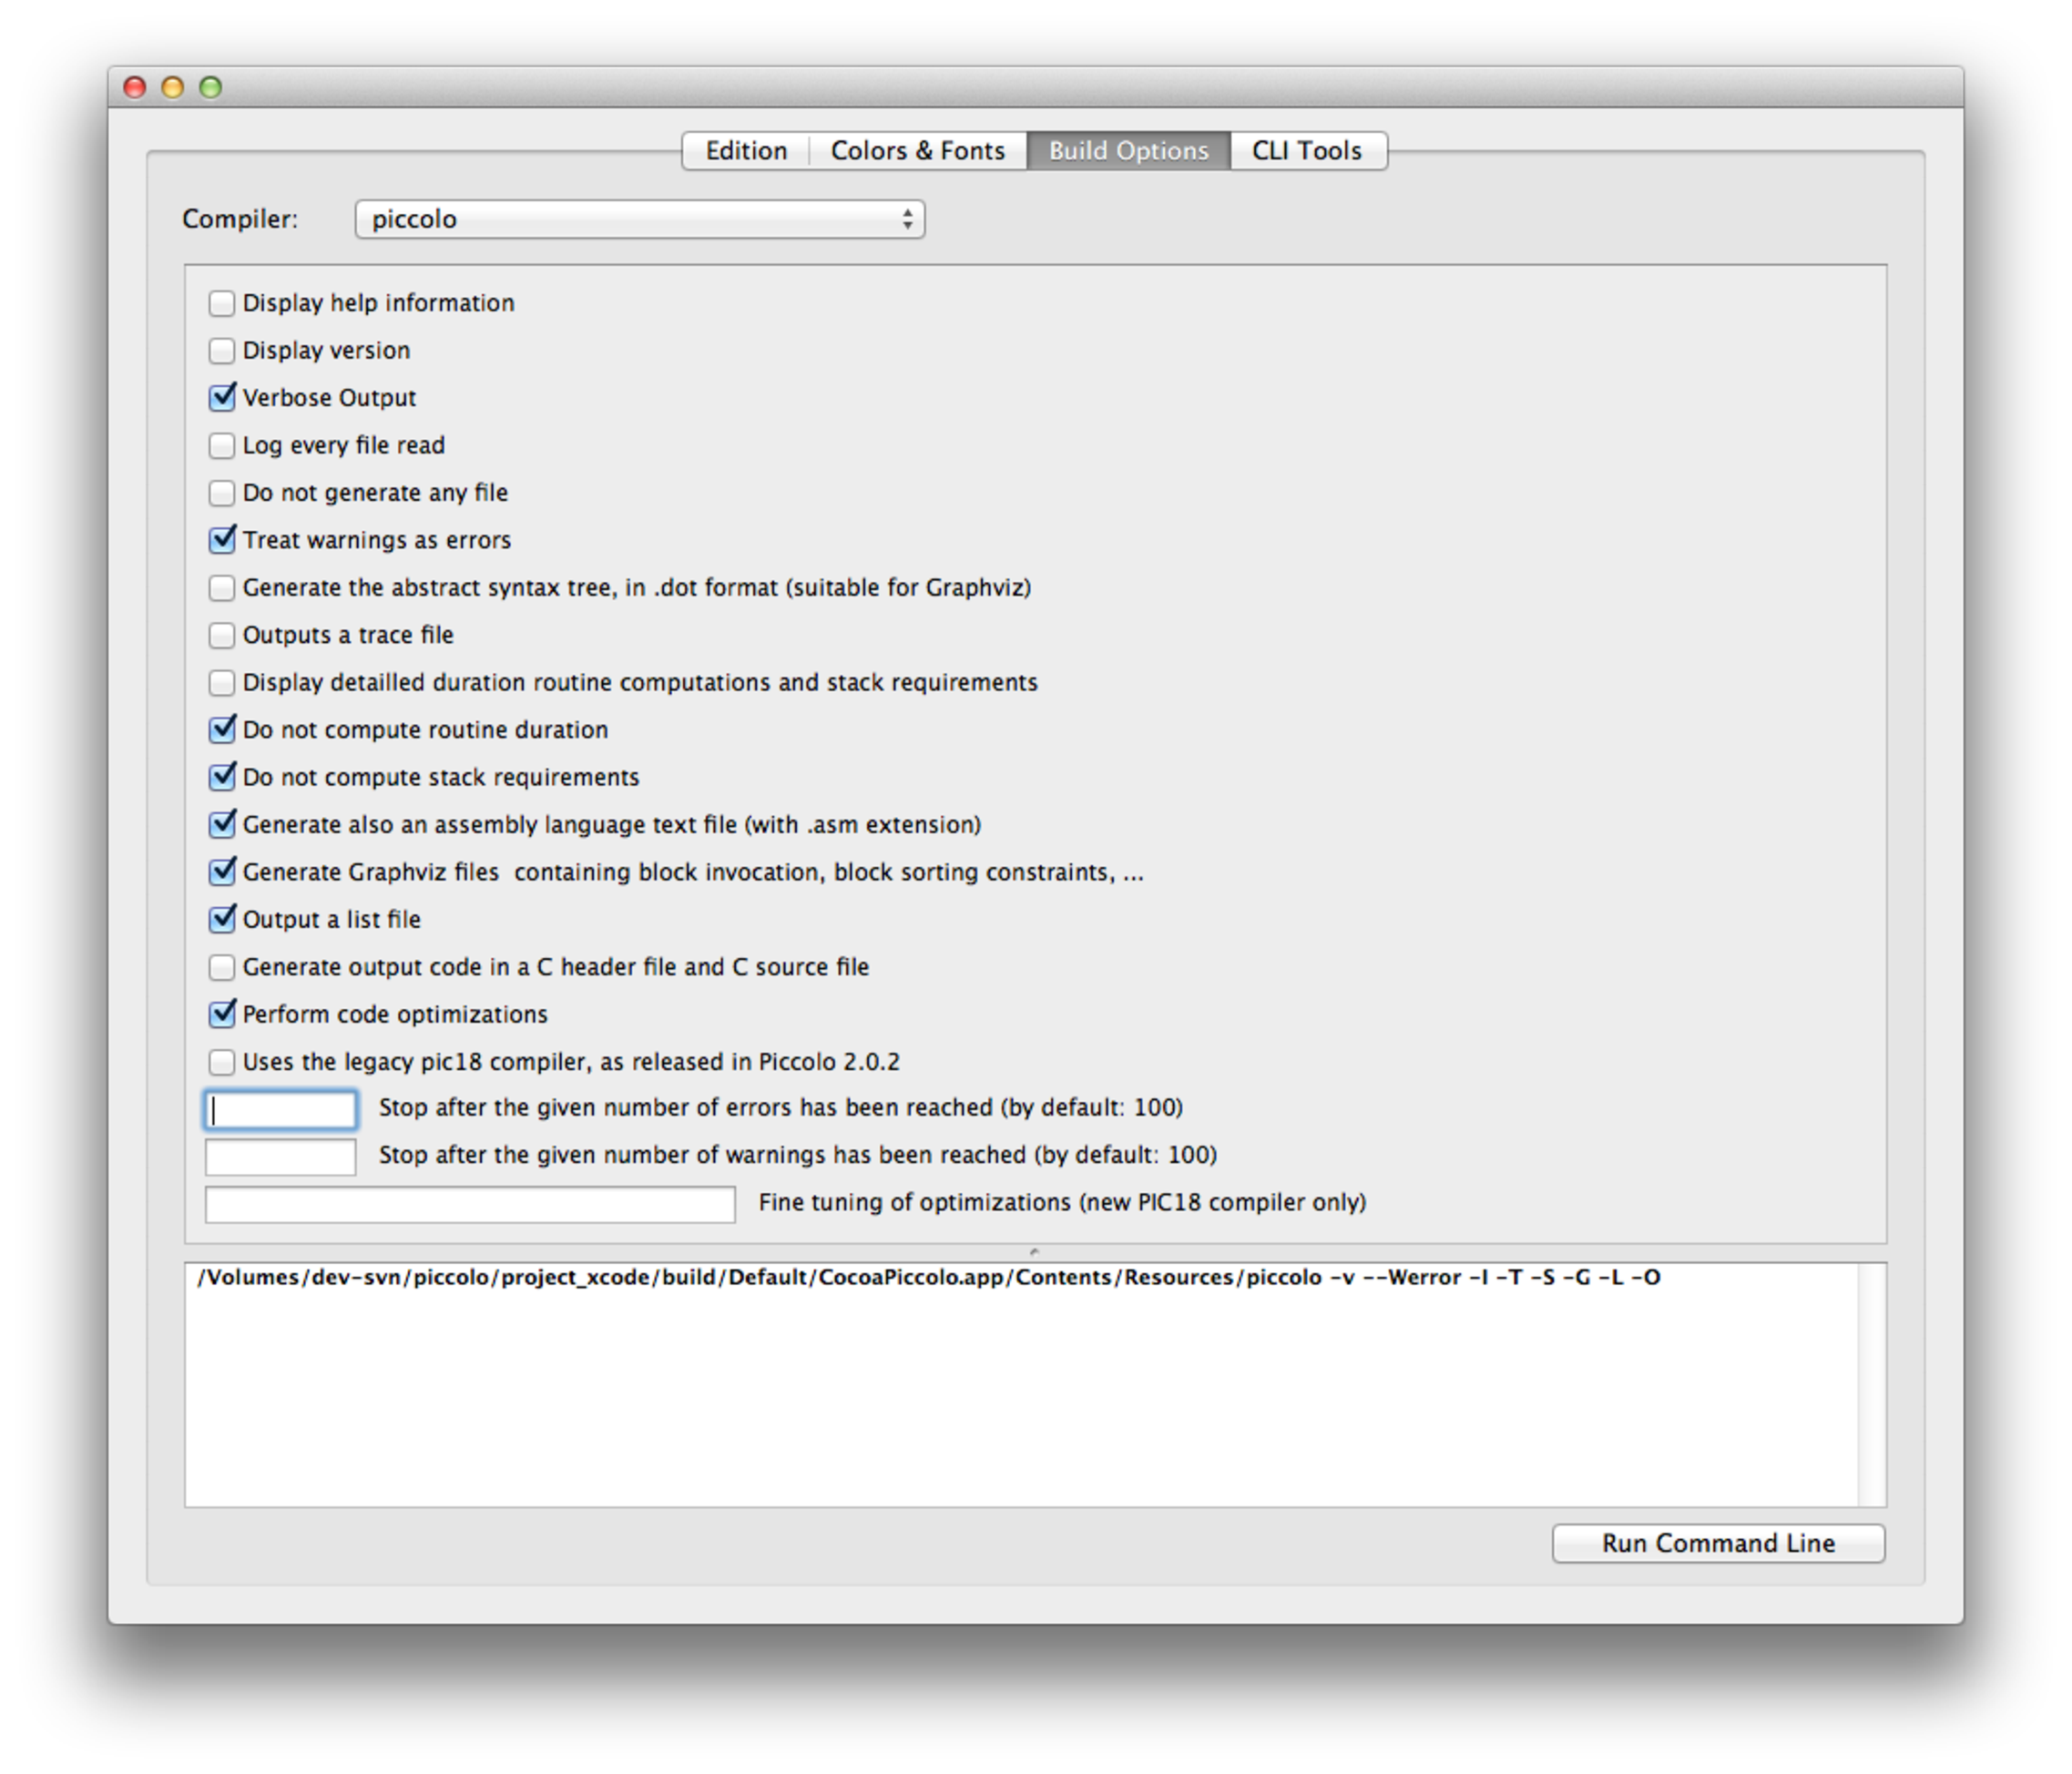
\includegraphics[width=1\textwidth]{images/build-options.pdf}
  \caption{Application Cocoa, options de compilation}
  \labelFigure{cocoaOptionsCompilation}
\end{figure}



\begin{figure}[!ht]
  \centering
  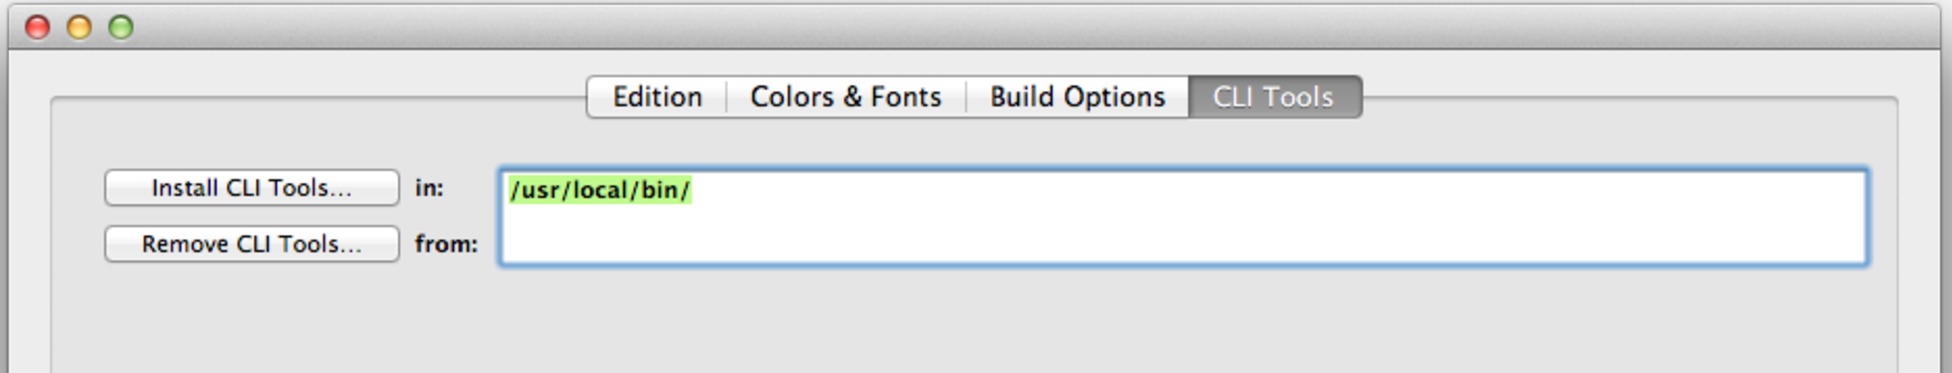
\includegraphics[width=1\textwidth]{images/installation-cli-tools.pdf}
  \caption{Application Cocoa, installation des outils en ligne de commande}
  \labelFigure{cocoaInstallationOutilsLigneCommande}
\end{figure}



\section{Options de la ligne de commande}

\subsectionLabel{Liste des options}{listeOptions}\index{Options de la ligne de commande}

Piccolo accepte un certain nombre d’options, qui sont détaillées dans les pages suivantes.

L’analyse des arguments de la ligne de commandes est simple :
\begin{itemize}
  \item tout argument qui commence par un « - » est une option ;
  \item tout argument qui ne commence pas par un « - » est considéré comme un fichier source Piccolo ;
  \item la seule extension acceptable pour un fichier source Piccolo est \texttt{.piccolo}.
\end{itemize}

En conséquence, un argument ne commençant pas par un « - » et n’ayant pas l’extension « .piccolo » déclenche une erreur.

L’ordre des options et des fichiers sources est quelconque. La ligne de commande est complètement analysée avant le traitement des fichiers sources.

Si plusieurs fichiers sources apparaissent dans la ligne de commande, ils sont traités dans leur ordre d’apparition.

{\bf Note pour Windows.} L’outil Piccolo pour Windows propose par défaut un dialogue invitant à entrer les références d’un fichier source si la ligne ne contient aucun fichier source (c’est le cas quand on double-clique sur l’icône de l’application). Une option « \texttt{-{-}no-dialog} », spécifique à cette plate forme, permet d'inhiber l’apparition du dialogue.

\subsubsection{Options générales}

\begin{description}
  \item[\texttt{-{-}version}] Affiche le numéro de version.

  \item[\texttt{-v}, \texttt{-{-}verbose}] Affiche des messages complémentaires sur le terminal. Par défaut, quand toutes les étapes se déroulent correctement, aucun message n’est affiché.

  \item[\texttt{-{-}no-color}] Les messages émis sur le terminal sont en texte pur, sans coloration.

  \item[\texttt{-{-}no-dialog}] (\emph{uniquement sur Windows}) L’outil Piccolo pour Windows propose par défaut un dialogue invitant à entrer les références d’un fichier source si la ligne ne contient aucun fichier source (c’est le cas quand on double-clique sur l’icône de l’application). Cette option permet d'inhiber l’apparition du dialogue.
\end{description}



\subsubsection{Options contrôlant le compilateur}




\begin{description}
  \item[\texttt{-{-}help}] Affiche la liste des options.

  \item[\texttt{-W}, \texttt{-{-}Werror}] Tout \emph{warning} est considéré comme une erreur. Cela peut être important dans un script, l’outil de commande renvoyant un code non nul si une ou plusieurs erreurs ont été détectées.

  \item[\texttt{-{-}max-errors=\emph{n}}] Stoppe après \emph{n} erreurs.

  \item[\texttt{-{-}max-warnings=\emph{n}}] Stoppe après \emph{n} alertes.

\end{description}



\subsubsectionLabel{Options contrôlant la génération}{optionsGeneration}


\begin{description}

  \item[\texttt{-o}, \texttt{-{-}optimize}] Effectue de manière itérative des optimisations du code produit.


  \item[\texttt{-F}, \texttt{-{-}optimization-flags}] Cette option concerne uniquement le compilateur pour \emph{pic18} des versions 3.x, elle n'a aucune impluence sur les compilateurs des \emph{baseline}, \emph{mid-range}. Cette option permet d'activer finement chacune des optimisations, l'option \texttt{-o} ci-dessus les activant toutes à la fois. À moins que vous soyez intéressé par le fonctionnement de l'optimiseur, vous n'avez pas à utiliser cette option. Elle s'utilise comme suit : par exemple, \texttt{-F=DER} active les optimisations \texttt{D}, \texttt{E} et \texttt{R} décrites ci-dessous. L'ordre d'apparition n'a aucune importance, il ne faut pas d'espace entre les lettres, plusieurs occurrences d'une même lettre ont le même effet qu'une seule occurrence. Les optimisations que vous pouvez ainsi activer sont :
\begin{itemize}
  \item \texttt{B} : les blocs sont ordonnés de façon à diminuer le nombre de sauts d'un bloc à l'autre ;
  \item \texttt{C} : les blocs sont regroupés en \emph{clusters} qui sont ensuite ordonnés de façon à diminuer le nombre de branchements relatifs à transformer en branchements absolu ; cette option n'est active que si l'option précédente \texttt{-B} l'est aussi ;
  \item \texttt{E} : l'appel à une routine constituée d'une instruction \assembleur{RETURN} est supprimé ;
  \item \texttt{e} : dans une instruction \texttt{computed rcall}, l'appel à une routine constituée d'une instruction \assembleur{RETURN} est remplacé par une instruction \texttt{BLANK} (c'est à dire un \assembleur{NOP} dont le code est \assembleur{0xF000}) ;
  \item \texttt{I} : l'appel à une routine constituée d'une seule instruction avant le \assembleur{RETURN} est remplacé par cette instruction ;
  \item \texttt{i} : dans une instruction \texttt{computed rcall}, l'appel à une routine constituée d'une seule instruction avant le \assembleur{RETURN} est remplacé par cette instruction ;
  \item \texttt{J} : une instruction \assembleur{RCALL}, \assembleur{CALL} ou \assembleur{JSR} suivie d'une instruction \assembleur{RETURN} est remplacée par une instruction \assembleur{BRA}, \assembleur{GOTO} ou \assembleur{JUMP} ;
  \item \texttt{M} : une instruction \assembleur{MOVLW k} suivie d'une instruction \assembleur{RETURN} est remplacée par une instruction \assembleur{RETLW k} ;
  \item \texttt{R} : l'appel à une routine constituée d'une instruction \assembleur{RETLW k} est remplacé par une instruction \assembleur{MOVLW k} ;
\end{itemize}



  \item[\texttt{-L}, \texttt{-{-}list}] Produit un fichier listing contenant de nombreux détails concernant la configuration, l’allocation de la RAM, les optimisations réalisées et la transformation des branchement relatifs en absolu. Ce fichier est écrit dans le même répertoire que le fichier source, porte le même nom, mais avec l’extension \texttt{.list}.

  \item[\texttt{-S}, \texttt{-{-}asm}] Si la compilation s’effectue sans erreur, engendre aussi un fichier texte assembleur, dans le même répertoire que le fichier source Piccolo, mais avec l’extension \texttt{.asm}.

  \item[\texttt{-n}, \texttt{-{-}no-file-generation}] Aucune écriture sur fichier n’a lieu : ceci permet de garantir que les fichiers de sortie ne seront pas engendrés. La tentative d’écrire un fichier est signalé par un \emph{warning}.

  \item[\texttt{-I}, \texttt{-{-}no-routine-duration}] Par défaut, Piccolo tente de calculer la durée d'exécution des routines (\emph{pic18} uniquement, \refChapterPage{pile-et-durees}). Cette option inhibe ce calcul.

  \item[\texttt{-T}, \texttt{-{-}no-stack-computation}] Par défaut, Piccolo tente de calculer les besoins en pile du programme (\emph{pic18} uniquement, \refChapterPage{pile-et-durees}). Cette option inhibe ce calcul.

  \item[\texttt{-d}, \texttt{-{-}detailled-computations}] Insère dans le fichier listing le détail des calculs de pile et de durée d'exécutions du programme (\emph{pic18} uniquement, \refChapterPage{pile-et-durees}.

  \item[\texttt{-G}, \texttt{-{-}generate-grahviz-files}] Engendre plusieurs fichiers d'extension \texttt{.dot} au format \emph{Graphviz} :
\begin{itemize}
\item \texttt{\emph{fichier-source}.blockInvocation.dot} : graphe d'appel entre les blocs ; les flèches en noires en trait plein sont les sauts qui peuvent être omis si les blocs sont consécutifs, en pointillé les sauts qui ne peuvent pas être omis, et les flèches rouges sont les appels par les instructions \piccolo{rcall} ou \piccolo{call} ; 
\item \texttt{\emph{fichier-source}.blockOrderingConstraints.dot} : contraintes d'ordre entre les blocs ; les flèches sont les sauts qui peuvent être omis si les blocs sont consécutifs ; 
\item \texttt{\emph{fichier-source}.blockOrderingConstraintsWoCycle.dot} : le graphe précédent dans lequel les circularités ont été élimininées, plus précisément les sauts d'un bloc vers un de ses dominateurs. 
\end{itemize}

  \item[\texttt{-C}, \texttt{-{-}output-c-files}] Engendre un fichier d'en-tête et un fichier C contenant le code objet résult de la compilation sous la forme de tableaux C.

\end{description}



\subsubsection{Options d'extraction des caractéristiques des micro-contrôleurs}

Piccolo embarque la description de tous les micro-contrôleurs supportés. Les options suivantes permettent d'extraire tout ou partie de ces informations.

\begin{description}


  \item[\texttt{-D}, \texttt{-{-}device-list}] Affiche sur le terminal la liste des micro-contrôleurs \emph{baseline}, \emph{mid-range} et \emph{pic18} supportés.

  \item[\texttt{-{-}baseline}] Affiche sur le terminal la liste des micro-contrôleurs \emph{baseline} supportés (voir \refSubsectionPage{listeBaseline}).

  \item[\texttt{-{-}midrange}] Affiche sur le terminal la liste des micro-contrôleurs \emph{mid-range} supportés (voir \refSubsectionPage{listeMidrange}).

  \item[\texttt{-{-}pic18}] Affiche sur le terminal la liste des micro-contrôleurs \emph{pic18} supportés (voir \refSubsectionPage{listePic18}).

  \item[\texttt{-F=string}, \texttt{-{-}configuration=string}] Affiche sur le terminal le détail des registres de configuration du micro-contrôleur désigné par \texttt{string}. Un exemple se trouve à la \refSubsectionPage{exempleOptionConfiguration}.

  \item[\texttt{-M=string}, \texttt{-{-}memory=string}] Affiche sur le terminal la composition des bancs de la RAM, la taille de la ROM et de l’EEPROM du micro-contrôleur désigné par \texttt{string}. Un exemple se trouve à la \refSubsectionPage{exempleOptionMemory}.

  \item[\texttt{-R=string}, \texttt{-{-}registers=string}] Affiche sur le terminal la liste alphabétique des registres spéciaux du micro-contrôleur désigné par \texttt{string}, ainsi que le nom de leurs bits. Un exemple se trouve à la \refSubsectionPage{exempleOptionRegisters}.

  \item[\texttt{-E=\emph{répertoire}}, \texttt{-{-}export=\emph{répertoire}}] Crée le dossier \emph{répertoire} et y place tous les fichiers de description des micro-contrôleurs \emph{baseline}, \emph{mid-range} et \emph{pic18}.

\end{description}



\subsubsection{Options contrôlant le débogage du compilateur}

Ces options ne sont pas utilisées lors de l'exploitation de Piccolo : elles permettent de déboguer le compilateur lui-même, et non pas le fichier source compilé.

\begin{description}

  \item[\texttt{-{-}log-file-read}] Affiche sur la console tout accès en lecture à un fichier.


  \item[\texttt{-{-}mode=\emph{nom}}] Contrôle l'opération du compilateur : si \emph{nom} est vide, le compilateur opère normalement. Si \emph{nom} est \texttt{lexical-only}, le compilateur affiche le résultat de l'analyse lexicale et s'arrête ; aucun fichier n'est engendré. Si \emph{nom} est \texttt{syntax-only}, le compilateur affiche le résultat de l'analyse syntaxique et s'arrête ; aucun fichier n'est engendré.



  \item[\texttt{-{-}trace}] Émet un fichier de trace de du compilateur. Format non documenté, utile uniquement pour déboguer le compilateur lui-même.


  \item[\texttt{-{-}output-concrete-syntax-tree}] Exporte dans un fichier l'arbre syntaxique concret du code source analysé sous la forme d'un graphe dont le format est compatible avec \emph{Graphviz}. Le nom du fichier de sortie est le nom du fichier source doté de l'extension complémentaire \texttt{.dot}.

\end{description}









\subsectionLabel{Exemple d'utilisation de l'option \texttt{-{}-memory}}{exempleOptionMemory}

Cette option affiche sur le terminal la composition des bancs de la RAM, la taille de la ROM et de l’EEPROM d'un micro-contrôleur.

Par exemple, pour le \texttt{18F448}, on écrit la ligne de commande :
\begin{quote}
  \texttt{piccolo -{}-memory=18F448}
\end{quote}

On obtient ainsi : 
\lstinputlisting[language=sortie]{files-from-piccolo/memory-18F448.txt}


\subsectionLabel{Exemple d'utilisation de l'option \texttt{-{}-registers}}{exempleOptionRegisters}

Cette option affiche sur le terminal la liste alphabétique des registres spéciaux d'un micro-contrôleur, ainsi que le nom de leurs bits.

Par exemple, pour le \texttt{12F683}, on écrit la ligne de commande :
\begin{quote}
  \texttt{piccolo -{}-registers=12F683}
\end{quote}

On obtient ainsi : 
\lstinputlisting[language=sortie]{files-from-piccolo/registers-12F683.txt}


\subsectionLabel{Exemple d'utilisation de l'option \texttt{-{}-configuration}}{exempleOptionConfiguration}

Cette option affiche sur le terminal le détail des registres de configuration d'un micro-contrôleur.

Par exemple, pour le \texttt{10F220}, on écrit la ligne de commande :
\begin{quote}
  \texttt{piccolo -{}-configuration=10F220}
\end{quote}

On obtient ainsi : 
\lstinputlisting[language=sortie]{files-from-piccolo/configuration-10F220.txt}









\section{Micro-contrôleurs supportés}

\subsectionLabel{Micro-contrôleurs \emph{baseline}}{listeBaseline}
\index{Baseline!Liste}

Pour connaître la liste des micro-contrôleurs \emph{baseline} pris en charge, utiliser l’option « \texttt{-{}-baseline} » :
\begin{quote}
\texttt{piccolo -{}-baseline}
\end{quote}

On obtient ainsi : 
\lstinputlisting[language=sortie]{files-from-piccolo/baseline.txt}




\subsectionLabel{Micro-contrôleurs \emph{mid-range}}{listeMidrange}
\index{Mid-range!Liste}



Pour connaître la liste des micro-contrôleurs \emph{mid-range} pris en charge, utiliser l’option « \texttt{-{}-midrange} » :
\begin{quote}
\texttt{piccolo -{}-midrange}
\end{quote}

On obtient ainsi : 
\lstinputlisting[language=sortie]{files-from-piccolo/midrange.txt}

\subsectionLabel{Micro-contrôleurs \emph{pic18}}{listePic18}
\index{Pic18!Liste}

Pour connaître la liste des micro-contrôleurs \emph{pic18} pris en charge, utiliser l’option « \texttt{-{}-pic18} » :
\begin{quote}
\texttt{piccolo -{}-pic18}
\end{quote}


On obtient ainsi : 
\lstinputlisting[language=sortie]{files-from-piccolo/pic18.txt}


%!TEX encoding = UTF-8 Unicode
%!TEX root = ../piccolo.tex


\chapter{Éléments lexicaux du langage Piccolo}

%--- Pour supprimer tout en-tête et pied de page sur la 1re page d'un chapitre
\thispagestyle{empty}


\section{Commentaires}

Un commentaire commence par un caractère dièse \pic+#+, et s’étend jusqu’à la fin de la ligne courante.

\section{Délimiteurs}

Piccolo définit les délimiteurs listés dans le \refTableau{delimiteursLangage}.

\begin{table}[!ht]
  \centering
  \begin{tabular}{ccccccccccccccccc}
    \hline
    \pic!*!  & \pic!*+! & \pic!,!  & \pic+!=+ & \pic!<=! & \pic!>=! & \pic!*-! & \pic!+*! & \pic!;! & \pic!:! & \pic!==! & \pic!<! & \pic!>! & \pic![! & \pic!]! \\
    \pic!.! & \pic+!+ & \pic!&! & \pic!|!  & \pic!}! & \pic!}! & \pic!(!  & \pic!)!  & \pic!/!  & \pic!-! & \pic!+! & \pic!^! & \pic!<<! & \pic!>>! & \pic!~!\\
    \pic!@! & \pic!%! & \pic!=! & \pic!?! & \pic!...!\\
  \end{tabular}
  \caption{Délimiteurs du langage Piccolo}
  \labelTableau{delimiteursLangage}
  \ligne
\end{table}

\section{Séparateurs}

Tout caractère dont le code ASCII est compris entre \texttt{0x01} et \texttt{0x20} est considéré comme un séparateur (ceci inclut donc la tabulation horizontale \texttt{HT} (\texttt{0x09}), le passage à la ligne \texttt{LF} (\texttt{0x0A}), le retour-chariot \texttt{CR} (\texttt{0x0D}), et l’espace (\texttt{0x20}).

\section{Identificateurs}
Un identificateur commence par une lettre (minuscule ou majuscule), qui est suivie par zéro, un ou plusieurs lettres (minuscules ou majuscules), chiffres décimaux, caractères \texttt{\_}.

La casse est significative pour les identificateurs.

\section{Mots réservés}
\index{Mots réservés}

Certains identificateurs sont réservés. La casse n’est pas significative pour les mots réservés, c’est à dire que les mots réservés peuvent être écrits indifféremment avec des lettres minuscules ou majuscules. Il y a deux classes de mots réservés :
\begin{itemize}
  \item ceux correspondants aux éléments du langage (\refSubsectionPage{motsReservesLangage}) ;
  \item ceux correspondants aux instructions exécutables (\refSubsectionPage{motsReservesInstruction}).
\end{itemize}

\subsectionLabel{Mots réservés correspondants aux éléments du langage}{motsReservesLangage}

Les mots réservés correspondant aux éléments du langage sont listés dans le \refTableau{motReservesLangage}. Dans tout ce document, ces mots réservés sont écrits en minuscule, gras et en bleu.


\begin{table}[!t]
  \centering
  \begin{tabular}{llllll}
   \pic!bank! & \pic!banksave! & \pic!banksel! & \pic!baseline! & \pic!block! \\
   \pic!bootloader! & \pic!byte! & \pic!case! & \pic!computed! & \pic!configuration! \\
   \pic!checkbank! & \pic!checknobank! & \pic!checkpic! & \pic!const! & \pic!contextsave! \\
   \pic!data! & \pic!do! & \pic!end! & \pic!else! & \pic!elsif!  \\
   \pic!ensures! & \pic!fast! & \pic!forever! & \pic!if!  & \pic!implements! \\
   \pic!include! & \pic!inline! & \pic!interrupt! & \pic!macro! & \pic!mark! \\
   \pic!midrange! & \pic!nobank! & \pic!noreturn! & \pic!page! & \pic!pic18! \\
   \pic!preserved! & \pic!ram! & \pic!requires! & \pic!rom! & \pic!routine! \\
   \pic!unused! & \pic!switch! & \pic!uses! & \pic!w! & \pic!while!\\
  \end{tabular}
  \caption{Mots réservés correspondant aux éléments du langage Piccolo}
  \labelTableau{motReservesLangage}
  \ligne
\end{table}





\subsectionLabel{Mots réservés correspondants aux instructions}{motsReservesInstruction}


Les mots réservés correspondant à des instructions exécutables sont listés dans le \refTableau{motReservesInstructions}. Dans tout ce document, ces mots réservés sont écrits en minuscule, gras et en marron. Pour les différencier, les instructions assembleur correspondantes sont écrites en majuscules.



\begin{table}[t]
  \centering
  \begin{tabular}{lllllll}
    \pic!addlw! & \pic!addwf! & \pic!addwfc! & \pic!andlw! & \pic!andwf! & \pic!bc! & \pic!bcf! \\
    \pic!bn! & \pic!bnc! & \pic!bnn! & \pic!bov! & \pic!bnov! & \pic!bnz! & \pic!bsf! \\
    \pic!bra! & \pic!btg! & \pic!bz! & \pic!call! & \pic!clrf! & \pic!clrw! & \pic!clrwdt! \\
    \pic!comf! & \pic!daw! & \pic!decf! & \pic!fnop! & \pic!goto! & \pic!incf! & \pic!iorlw! \\
    \pic!iorwf! & \pic!jsr! & \pic!jump! & \pic!lfsr! & \pic!ldataptr! & \pic!ltblptr! & \pic!mnop! \\
    \pic!movf! & \pic!movff! & \pic!movlw! & \pic!movwf! & \pic!mullw! & \pic!mulwf! & \pic!negf! \\
    \pic!nop! & \pic!pop! & \pic!option! & \pic!push! & \pic!rcall! & \pic!reset! & \pic!retlw! \\
    \pic!rlcf! & \pic!rlf! & \pic!rlncf! & \pic!rrcf! & \pic!rrf! & \pic!rrncf! & \pic!setf! \\
    \pic!sleep! & \pic!subfwb! & \pic!sublw! & \pic!subwf! & \pic!subwfb! & \pic!swapf! & \pic!tblrd!\\
    \pic!tblwt! & \pic!tris! & \pic!xorlw! & \pic!xorwf! & & & \\
\end{tabular}
  \caption{Mots réservés correspondant aux instructions exécutables Piccolo}
  \labelTableau{motReservesInstructions}
  \ligne
\end{table}



\section{Constante chaîne de caractères}

Comme en C, les chaînes de caractères sont délimitées par des caractères \texttt{"}. Les séquences d’échappement suivantes sont acceptées : \texttt{\textbackslash f}, \texttt{\textbackslash n}, \texttt{\textbackslash r}, \texttt{\textbackslash v}, \texttt{\textbackslash\textbackslash}, \texttt{\textbackslash\textquotedbl}, \texttt{\textbackslash\textquotesingle}, \texttt{\textbackslash0}.

\section{Constante caractère}

Comme en C, les caractères sont délimités par des caractères « \texttt{\textquotesingle} ». Par exemple :\pic!'A'!, \pic!'+'!.


Les séquences d’échappement suivantes sont acceptées : \pic!'\f'!, \pic!'\n', !\pic!'\r'!, \pic!'\v'!, \pic!'\\'!, \pic!'\''!, \pic!'\0'!.

\section{Constante entière}

Vous pouvez écrire les constantes entières en décimal, en hexadécimal ou en binaire. 

\textbf{Décimal.} Une constante entière décimale commence par un chiffre décimal, et est suivie par zéro, un ou plusieurs chiffres décimaux, ou caractères \texttt{\_}.

\textbf{Hexadécimal.} Un chiffre hexadécimal est soit un chiffre décimal, soit une lettre entre \texttt{a} et \texttt{f}, écrite indifféremment en minuscule ou en majuscule. Une constante hexadécimale commence par la séquence \texttt{0x} », et est suivie par un ou plusieurs chiffres hexadécimal, ou caractères \texttt{\_}.

\textbf{Binaire.} Une constante entière binaire commence par la séquence \texttt{0b} suivie par un ou plusieurs chiffres binaires, \texttt{0} ou \texttt{1}, ou le caractère \texttt{\_}.

Dans une constante entière, écrite en binaire, décimal ou en hexadécimal, le caractère \texttt{\_} peut servir de séparateur ; on peut ainsi écrire indifféremment : \pic!123!, \pic!1_23!, \pic!1_2_3!, \pic!1___23!, \dots

Attention :
\begin{itemize}
  \item contrairement au C, un nombre qui commence par un zéro est un nombre écrit en décimal ;
  \item contrairement à l’assembleur PIC, le préfixe \texttt{0x} est indispensable pour écrire un nombre en hexadécimal.
\end{itemize}

\section{Format}

Le format est libre, la fin de ligne n’est pas significative (sauf pour les commentaires, qui commencent par un caractère dièse \texttt{\#}, et s’étendent jusqu’à la fin de la ligne courante). Le compilateur accepte de manière indifférente que les fins de ligne soient codés par un caractère LF (\texttt{0x0A}), un caractère CR (\texttt{0x0D}), ou par la séquence CRLF (\texttt{0x0D}, \texttt{0x0A}).

À partir de la version 2.0.2, les commentaires commençant par \texttt{\#!} sont capturés par l'application CocoaPiccolo pour être affichés dans le menu \emph{popup} d'accès aux routines.


%!TEX encoding = UTF-8 Unicode
%!TEX root = ../piccolo.tex


\chapter{Programmes pour baseline}

%--- Pour supprimer tout en-tête et pied de page sur la 1re page d'un chapitre
\thispagestyle{empty}




\section{Structure d’un programme pour baseline}

Un programme Piccolo pour \emph{baseline} a la structure suivante :

\begin{piccolo}
baseline nom "nom_composant" :
  liste_de_sections
end
\end{piccolo}


Dans l’en-tête :
\begin{itemize}
  \item le nom « \emph{nom} » est le nom du fichier (sans son extension) qui contient ce texte source ;
  \item le nom du composant « \emph{nom\_composant} » doit être exactement le nom de l’un des composants supportés (pour obtenir la liste des \emph{baseline} pris en charge, utiliser l’option « \texttt{-{}-baseline} », voir \refSubsectionPage{listeBaseline}).
\end{itemize}


Le corps du programme est constitué d’une liste non ordonnée de sections. Les sections disponibles sont listées dans le \refTableau{sectionsBaseline}.
\begin{table}[!t]
  \centering
%  \rowcolors{2}{\fondTableau}{}
  \begin{tabular}{p{5cm}lll}
    \textbf{Type de section} & \textbf{Mot-clés introductifs} & \textbf{Référence}\\
    Configuration & \pic!configuration!\index{Mot réservé!configuration} & \refChapterPage{configuration}\\
    \hdashline
    Définition de variable & \pic!ram!\index{Mot réservé!ram} & \refChapterPage{ram}\\
    \hdashline
    Déclaration de variable inutilisée & \pic!unused byte!\index{Mot réservé!unused} & \refSectionPage{sectionUnusedByte} \\
    \hdashline
    Définition de constante & \pic!const!\index{Mot réservé!const} & \refChapterPage{constante}\\
    \hdashline
    Définition de routine régulière & \pic!routine!\index{Mot réservé!routine} & \refSectionPage{routineBaseline}\\
    \hdashline
    Définition de routine sans retour & \pic!noreturn routine!\index{Mot réservé!noreturn} & \refSectionPage{routineBaseline}\\
    \hdashline
    Routine inutilisée & \pic!unused routine!\index{Mot réservé!unused} & \refSubsectionPage{routineInutiliseeBaseline} \\
    \hdashline
    Inclusion  & \pic!include!\index{Mot réservé!include} & \refSectionPage{sectionIncludeBaseline} \\
  \end{tabular}
  \caption{Les sections d'un programme pour \emph{baseline}}
  \labelTableau{sectionsBaseline}
  \ligne
\end{table}




\sectionLabel{Routines baseline}{routineBaseline}

Les routines définissent le code exécutable de votre programme. L’une d’entre elles doit s’appeler \pic!main! : c’est la routine qui s’exécute au démarrage. Il y a deux types de routine, les routines \emph{régulières} et les routines \emph{sans retour}.


L’ordre des déclarations des routines est quelconque, il est possible d’appeler une routine qui est déclarée après l’instruction d’appel. Simplement Piccolo engendrera leur code dans leur ordre d’apparition. 

\textbf{Routine et pages de la mémoire programme.} Un problème important en Piccolo \emph{baseline} est la gestion des pages de la mémoire programme (voir \refSectionPage{gestionPagesBaseline}).

\textbf{Liste d’instructions d’une routine.} Elle est structurée : Piccolo définit des instructions de sélection et de répétition : cela signifie que vous ne pouvez pas déclarer d’étiquette, ni utiliser de \pic!goto! pour effectuer des branchements à l’intérieur d’une routine.


\subsectionLabel{Routine régulière}{routineReguliereBaseline}
\index{Routine régulière!baseline}

C'est un sous-programme. Comme l'assembleur \emph{baseline} ne définit pas d'instruction \assembleur{RETURN} mais uniquement une instruction \assembleur{RETLW}, une routine régulière doit se terminer par une instruction \pic!movlw! (voir ci-après). Une routine régulière est déclarée par :
\begin{piccolo}
routine maRoutine ... {
  ...
  movlw ...
}
\end{piccolo}

\pic!maRoutine! est le nom de la routine, celui qui sera nommé dans un instruction d’appel de routine. Entre les accolades \pic!{! et \pic!}!, apparaît la liste des instructions.

\textbf{Appel d’une routine régulière.} Utiliser l'instruction \pic!call! ou l'instruction \pic!jsr! (\refSectionPage{gestionPagesBaseline}).

\textbf{Dernière instruction d’une routine régulière.} Une particularité du jeu d'instructions des \emph{baseline} est qu'il ne possède pas d'instruction \assembleur{RETURN}, mais une instruction \assembleur{RETLW} qui combine retour de sous-programme et chargement immédiat de \pic!W!. Piccolo ne définit pas l'instruction \assembleur{RETLW}, mais définit \pic!movlw! : c'est le compilateur Piccolo qui repère une instruction \assembleur{MOVLW} comme dernière instruction d'une routine, et qui la transforme en \assembleur{RETLW}.

En conséquence, la liste des instructions d'une routine régulière ne peut pas être vide. Elle doit comprendre au moins une instruction. D'une manière générale, la dernière instruction d'une routine régulière peut être :
\begin{itemize}
  \item une instruction \pic!movlw! ; le compilateur Piccolo la transformera en \assembleur{RETLW} ;
  \item une instruction \pic!call! ou une instruction \pic!jsr! vers une routine régulière ; le compilateur Piccolo la transformera en \assembleur{GOTO} ;
  \item une instruction \pic!if! structurée dont toutes les branches se terminent soit par une instruction \pic!movlw!, soit par une instruction \pic!call! vers une routine régulière, soit une autre instruction \pic!if! structurée.
\end{itemize}

Voici quelques exemples de routines régulières Piccolo et leur traduction en assembleur. Noter qu'il s'agit du code engendré sans aucune optimisation.
\begin{multicols}{2}
\textbf{Routine Piccolo}
\begin{piccolo}
routine maRoutine {
  movlw 45
}
\end{piccolo}
\columnbreak
\textbf{Traduction assembleur}
\begin{lstlisting}[language=assembleur]
maRoutine:
  RETLW 0x2D
\end{lstlisting}
\end{multicols}

\begin{multicols}{2}
\textbf{Routine Piccolo}
\begin{piccolo}
routine maRoutine {
  call autreRoutineReguliere
}
\end{piccolo}
\columnbreak
\textbf{Traduction assembleur}
\begin{lstlisting}[language=assembleur]
maRoutine:
  GOTO autreRoutineReguliere
\end{lstlisting}
\end{multicols}


\begin{multicols}{2}
\textbf{Routine Piccolo}
\begin{piccolo}
routine maRoutine {
  if (STATUS.Z)
    call autreRoutineReguliere
  else
    movlw 45
  end
}
\end{piccolo}
\columnbreak
\textbf{Traduction assembleur}
\begin{lstlisting}[language=assembleur]
maRoutine:
  BTFSS STATUS, 2
  GOTO _label_0
  GOTO autreRoutineReguliere
_label_0:
  RETLW 0x2D
\end{lstlisting}
\end{multicols}


\subsection{Routine sans retour}
\index{Routine sans retour!baseline}

L’exécution ne revient pas jamais à l’appelant. Ce type de routine doit donc se terminer par des constructions particulières qui assurent le non-retour : une boucle infinie, un branchement \pic!goto! ou \pic!jump! vers une autre routine sans retour.

Une routine sans retour doit être déclarée avec qualificatif \pic!noreturn! :
\begin{piccolo}
noreturn routine maRoutine ... {
  ...
}
\end{piccolo}

\textbf{Appel d’une routine sans retour.} Utiliser \pic!goto! ou l'instruction \pic!jump! (\refSectionPage{gestionPagesBaseline}).


\textbf{Déclaration de la routine \pic!main!.} Dans un programme, il doit exister une et une seule routine \pic!main!, qui doit être déclarée comme suit :

\begin{piccolo}
noreturn routine main {
   liste_instructions
}

\end{piccolo}

Le compilateur Piccolo place cette routine au début de la ROM, de façon qu'elle soit exécutée au démarrage du micro-contrôleur.


\textbf{Comment terminer une routine sans retour.} La dernière instruction de la liste des instructions d’une routine sans retour doit être :
\begin{itemize}
  \item une instruction de répétition infinie (\refSectionPage{repetitionInfinie}) ;
  \item un appel vers une autre routine sans retour, au moyen d’un \pic!goto! ou d'un \pic!jump! ;
  \item une instruction conditionnelle structurée, dont toutes les branches présentent comme dernière instruction les instructions d’appel d’un routine sans retour, un branchement calculé (comme évoqué ci-dessus), ou encore une instruction conditionnelle structurée, dont toutes les branches, etc.

\end{itemize}

Exemple simple : la dernière instruction est une boucle infinie :
\begin{piccolo}
noreturn routine maRoutine {
  ...
  forever
    ...
  end
}
\end{piccolo}

Exemple simple : la dernière instruction est un branchement vers une routine sans retour :
\begin{piccolo}
noreturn routine maRoutine {
  ...
  goto autreRoutineSansRetour
}
\end{piccolo}


La dernière instruction est un \pic!if! dont aucune des branches ne se termine (\pic!r1! est une routine sans retour) :
\begin{piccolo}
noreturn routine maRoutine {
  if (...)
    ...
    goto r1
  else
    ...
    forever
      ...
    end
  end
}

\end{piccolo}


La dernière instruction est un \pic!if! dont la première branche se termine elle même par un \pic!if! dont les deux branches se terminent par des branchements vers des routines sans retour :
\begin{piccolo}
noreturn routine maRoutine {
  if (...)
    ...
    if (...)
      ...
      goto r1
    else
      ...
      goto r2
    end
  else
    ...
    goto r3
  end
}
\end{piccolo}




\subsectionLabel{Routine inutilisée}{routineInutiliseeBaseline}

Par défaut à partir de la version 3.0.2, Piccolo détecte les routines inutilisées. Un \emph{warning} est déclenché pour chaque routine inutilisée.

Pour inhiber ce \emph{warning}, on utilise la déclaration \pic!unused routine! :

\begin{piccolo}
baseline exemple "16F57" :
routine uneRoutine page 0 {
  movlw 0
}

unused routine uneRoutine
 
noreturn routine main page 0 {
  forever
  end
}

end
\end{piccolo}

La déclaration \pic!unused routine! peut apparaître avant ou après la déclaration des routines qu'elle nomme ; plusieurs routines peuvent être nommées, en séparant leurs noms par une virgule :
\begin{piccolo}
unused routine routine1, routine2
\end{piccolo}



\section{Les instructions}
\index{Baseline!Instructions machine}

Elles sont de deux types (la distinction est importante pour l’instruction \emph{conditionnelle simple}) :
\begin{itemize}
  \item les instructions simples ;
  \item les instructions composées.

\end{itemize}


\textbf{Les instructions simples.} Elles correspondent à une partie des instructions machine. Attention, pour certaines, la syntaxe n'est pas exactement la même que celle de l'instruction assembleur correspondante.

Le \refTableau{instructionsAssembleurBaseline} donnent la liste des instructions machine \emph{baseline} et les liens vers les sections précisant leur prise en charge en Piccolo.

 
\begin{table}[!t]
  \centering
  \small
%  \rowcolors{2}{\fondTableau}{}
  \begin{tabular}{lll}
    \textbf{Instruction} & \textbf{Description} & \textbf{Référence en Piccolo}\\
    \assembleur{ADDWF f, d} & Add W and f & \refSubsectionPage{instructionsBaselineNommantRegistreEtW} \\
    \hdashline
    \assembleur{ANDLW k} & And Literal with W & \refSubsectionPage{opBaselineImmediate}\\
    \hdashline
    \assembleur{ANDWF f, d} & And W with f & \refSubsectionPage{instructionsBaselineNommantRegistreEtW}\\
    \hdashline
    \assembleur{BCF f, b} & Bit Clear f & \refSubsectionPage{opBaselineAffectationBit} \\
    \hdashline
    \assembleur{BSF f, b} & Bit Set f & \refSubsectionPage{opBaselineAffectationBit} \\
    \hdashline
    \assembleur{BTFSC f, b} & Bit Test f, Skip if Clear & \refSubsectionPage{instructionsBaselineIntrouvables}\\
    \hdashline
    \assembleur{BTFSS f, b} & Bit Test f, Skip if Set & \refSubsectionPage{instructionsBaselineIntrouvables}\\
    \hdashline
    \assembleur{CALL k} & Call Subroutine &  \refSubsectionPage{appelRoutineReguliereBaseline} \\
    \hdashline
    \assembleur{CLRF f} & Clear f & \refSubsectionPage{instructionsBaseLineNommantRegistre} \\
    \hdashline
    \assembleur{CLRW} & Clear W & \refSubsectionPage{operationsBaselineIdentiquesAssembleur}\\
    \hdashline
    \assembleur{CLRWDT} & Clear Watchdog Timer & \refSubsectionPage{operationsBaselineIdentiquesAssembleur}\\
    \hdashline
    \assembleur{COMF f, d} & Complement f & \refSubsectionPage{instructionsBaselineNommantRegistreEtW}\\
    \hdashline
    \assembleur{DECF f, d} & Decrement f & \refSubsectionPage{instructionsBaselineNommantRegistreEtW}\\
    \hdashline
    \assembleur{DECFSZ f, d} & Decrement f, Skip if 0 & \refSubsectionPage{instructionsBaselineIntrouvables}\\
    \hdashline
    \assembleur{GOTO k} & Go to Address & \refSubsectionPage{appelRoutineSansRetourBaseline} \\
    \hdashline
    \assembleur{INCF f, d} & Decrement f & \refSubsectionPage{instructionsBaselineNommantRegistreEtW}\\
    \hdashline
    \assembleur{INCFSZ f, d} & Increment f, Skip if 0 & \refSubsectionPage{instructionsBaselineIntrouvables}\\
    \hdashline
    \assembleur{IORLW k} & Inclusive OR Literal with W & \refSubsectionPage{opBaselineImmediate}\\
    \hdashline
    \assembleur{IORWF f, d} & Inclusive OR W with f & \refSubsectionPage{instructionsBaselineNommantRegistreEtW}\\
    \hdashline
    \assembleur{MOVF f, d} & Move f & \refSubsectionPage{instructionsBaselineNommantRegistreEtW}\\
    \hdashline
    \assembleur{MOVLW k} & Move Literal to W & \refSubsectionPage{opBaselineImmediate}\\
    \hdashline
    \assembleur{MOVWF f} & Move W to f & \refSubsectionPage{instructionsBaseLineNommantRegistre} \\
    \hdashline
    \assembleur{NOP} & No Operation & \refSubsectionPage{operationsBaselineIdentiquesAssembleur}\\
    \hdashline
    \assembleur{RETLW k} & Return with Literal in W & \refSubsectionPage{instructionsBaselineIntrouvables}\\
    \hdashline
    \assembleur{RLF f, d} & Rotate Left f through Carry & \refSubsectionPage{instructionsBaselineNommantRegistreEtW}\\
    \hdashline
    \assembleur{RRF f, d} & Rotate Right f through Carry & \refSubsectionPage{instructionsBaselineNommantRegistreEtW}\\
    \hdashline
    \assembleur{SLEEP} & Go into Standby Mode & \refSubsectionPage{operationsBaselineIdentiquesAssembleur}\\
    \hdashline
    \assembleur{SUBWF f, d} & Substract W from f & \refSubsectionPage{instructionsBaselineNommantRegistreEtW}\\
    \hdashline
    \assembleur{SWAPF f, d} & Swap Nibbles in f & \refSubsectionPage{instructionsBaselineNommantRegistreEtW}\\
    \hdashline
    \assembleur{TRIS f} & Load TRIS register & \refSubsectionPage{instructionTRIS}\\
    \hdashline
    \assembleur{XORLW k} & Exclusive OR Literal with W & \refSubsectionPage{opBaselineImmediate}\\
    \hdashline
    \assembleur{XORWF f, d} & Exclusive OR W with f & \refSubsectionPage{instructionsBaselineNommantRegistreEtW}\\
  \end{tabular}
  \caption{Instructions machine des \emph{baseline}}
  \labelTableau{instructionsAssembleurBaseline}
  \ligne
\end{table}






\textbf{Les instructions composées.} Piccolo définit les instructions suivantes :
\begin{itemize}
  \item l'instruction \pic!mnop! (\refSectionPage{instructionMNOP}) ;
  \item l'instruction conditionnelle simple (\refSectionPage{instructionConditionnelleSimple}) ;
  \item l'instruction conditionnelle structurée (\refSectionPage{instructionConditionnelleStructuree}) ;
  \item l'instruction répétitive (\refSectionPage{instructionRepetitive}) ;
  \item l'instruction de répétition infinie (\refSectionPage{repetitionInfinie}) ;
  \item l'instruction de répétition statique (\refSectionPage{repetitionStatique}) ;
  \item l'instruction d'appel de routine régulière \pic!jsr! (\refSectionPage{gestionPagesBaseline}) ;
  \item l'instruction d'appel de routine sans retour \pic!jump! (\refSectionPage{gestionPagesBaseline}) ;
\end{itemize}




\subsectionLabel{Les instructions que vous ne trouverez pas en Piccolo}{instructionsBaselineIntrouvables}

Elles n’existent pas en Piccolo parce qu’elles sont remplacées par des constructions structurées, ou bien engendrées automatiquement lors de la compilation.

Voici leur liste avec les liens vers les sections appropriées :\begin{itemize}
  \item \assembleur{BTFSC}, \assembleur{BTFSS}, \assembleur{DECFSZ} et \assembleur{INCFSZ} : ces instructions sont engendrées par l’instruction conditionnelle simple, l’instruction conditionnelle structurée et l’instruction répétitive (\refSubsectionPage{conditionsElementairesBaselineMidRange}) ;
  \item \assembleur{RETLW} : utiliser une instruction \assembleur{MOVLW}, et c’est le compilateur Piccolo qui la remplacera par une instruction \assembleur{RETLW k} (\refSubsectionPage{routineReguliereBaseline}).

\end{itemize}





\sectionLabel{Les instructions simples}{instructionsSimplesBaseline}


\subsectionLabel{Instructions nommant un registre}{instructionsBaseLineNommantRegistre}

Ce sont les instructions listées dans le \refTableau{operationsBaselineNommantUnRegistre}.



\begin{table}[!t]
  \centering
  \small
%  \rowcolors{2}{\fondTableau}{}
  \begin{tabular}{lll}
    \textbf{Assembleur} & \textbf{Description} & \textbf{Écriture en Piccolo}\\
    \assembleur{CLRF f} & Clear f & \pic!clrf f! \\
    \hdashline
    \assembleur{MOVWF f} & Move f & \pic!movwf f! \\
  \end{tabular}
  \caption{Opérations \emph{baseline} nommant un registre}
  \labelTableau{operationsBaselineNommantUnRegistre}
  \ligne
\end{table}








\subsectionLabel{Instructions nommant un registre, et optionnellement \texttt{W}}{instructionsBaselineNommantRegistreEtW}

Ces instructions, ainsi que le traduction en Piccolo, sont listées dans le \refTableau{instructionsBaselineRegistreEtW}. En assembleur, elles nomment deux opérandes :
\begin{itemize}
  \item \assembleur{f} : désigne le registre, il en est de même en Piccolo ;
  \item \assembleur{d} : optionnel en Piccolo ; si absent, le registre \assembleur{f} est destination de l'opération, si égal à \pic!W!, c'est le registre \pic!W! qui est destinaire.
\end{itemize}


\begin{table}[!t]
  \centering
  \small
%  \rowcolors{2}{\fondTableau}{}
  \begin{tabular}{llll}
     &  & \multicolumn{2}{l}{\textbf{En Piccolo, destination :}} \\
    \textbf{Assembleur} & \textbf{Description} & \textbf{f} & \textbf{W}\\
    \assembleur{ADDWF f, d} & Add W and f & \pic!addwf f!  & \pic!addwf f, W! \\
    \hdashline
    \assembleur{ANDWF f, d} & And W with f & \pic!andwf f! & \pic!andwf f, W!\\
    \hdashline
    \assembleur{COMF f, d} & Complement f & \pic!comf f! & \pic!comf f, W!\\
    \hdashline
    \assembleur{DECF f, d} & Decrement f & \pic!decf f! & \pic!decf f, W!\\
    \hdashline
    \assembleur{INCF f, d} & Increment f & \pic!incf f! & \pic!incf f, W!\\
    \hdashline
    \assembleur{IORWF f, d} & Inclusive OR W with f & \pic!iorwf f! & \pic!iorwf f, W!\\
    \hdashline
    \assembleur{MOVF f, d} & Move f & \pic!movf f! & \pic!movf f, W!\\
    \hdashline
    \assembleur{RLF f, d} & Rotate Left f through Carry & \pic!rlf f! & \pic!rlf f, W!\\
    \hdashline
    \assembleur{RRF f, d} & Rotate Right f through Carry & \pic!rrf f! & \pic!rrf f, W!\\
    \hdashline
    \assembleur{SUBWF f, d} & Substract W from f & \pic!subwf f! & \pic!subwf f, W!\\
    \hdashline
    \assembleur{SWAPF f, d} & Swap Nibbles in f & \pic!swapf f! & \pic!swapf f, W!\\
    \hdashline
    \assembleur{XORWF f, d} & Exclusive OR W with f & \pic!xorwf f! & \pic!xorwf f, W!\\
  \end{tabular}
  \caption{Instructions \emph{baseline} nommant un registre, et optionnellement \texttt{W}}
  \labelTableau{instructionsBaselineRegistreEtW}
  \ligne
\end{table}


\subsectionLabel{Opérations d'affectation de bit}{opBaselineAffectationBit}

Ces instructions Piccolo correspondent aux instructions machine \assembleur{BCF} et \assembleur{BSF} (\refTableau{operationsBaselineAffectationBit}).

\begin{table}[!t]
  \centering
  \small
%  \rowcolors{2}{\fondTableau}{}
  \begin{tabular}{lll}
    \textbf{Assembleur} & \textbf{Description} & \textbf{Écriture en Piccolo}\\
    \assembleur{BCF f, b} & Bit Clear f & \pic!bcf f.b! \\
    \hdashline
    \assembleur{BSF f, b} & Bit Set f & \pic!bsf f.b! \\
  \end{tabular}
  \caption{Opérations \emph{baseline} sur un bit d'un registre}
  \labelTableau{operationsBaselineAffectationBit}
  \ligne
\end{table}

En Piccolo, ces instructions ont toujours deux arguments :
\begin{itemize}
  \item le premier argument est une référence à un registre (\refSectionPage{referenceRegistre}) ;
  \item le second est le bit concerné, précédé par un point.
\end{itemize}

Pour désigner le bit concerné, vous pouvez utiliser un nombre compris entre 0 et 7. Par exemple :
\begin{piccolo}
bcf maVariable.3
\end{piccolo}


Vous pouvez utiliser une expression statique pour désigner un numéro de bit, à condition de la mettre entre parenthèses :
\begin{piccolo}
bcf maVariable.(2 + 1)
\end{piccolo}


Si le registre a été défini en déclarant des noms de bit :
\begin{piccolo}
ram ... {
  byte maVariable <a, -, b [3], -, -, ->
}
\end{piccolo}

Vous pouvez utiliser l’un de ces noms comme second argument :
\begin{piccolo}
bcf maVariable.a # a designe le bit 7
\end{piccolo}
ou encore
\begin{piccolo}
bcf maVariable.b [1] # b[1] designe le bit 4
\end{piccolo}

Vous pouvez de cette façon accéder aux bits des registres spéciaux. Pour connaître la liste des registres de contrôle, utilisez l’option \texttt{-{}-registers} (ou sa version courte \texttt{-R}), comme décrite à la \refSubsectionPage{exempleOptionRegisters} ; par exemple : \texttt{piccolo -R=10F220}.


\subsectionLabel{Opérations littérales avec \texttt{W}}{opBaselineImmediate}

Ces opérations sont listées dans le \refTableau{operationsLiteralesBaselineAvecW}. L’instruction \assembleur{RETLW k} n’existe pas en Piccolo, l’optimiseur repérera une instruction \assembleur{MOVLW k} en fin de routine et la transformera en \assembleur{RETLW k}.

En Piccolo, $k$ est une \emph{expression statique}. Une expression statique est une expression dont la valeur est calculée à la compilation. Sa forme générale est présentée à la \refSectionPage{expressionImmediate}. Le compilateur effectue tous les calculs d'une expression statique avec des nombres entiers 32 bits signés.

Pour être valide dans les opérations statiques avec \pic!W!, le résultat devra être :
\begin{itemize}
  \item soit un nombre positif inférieur ou égal à 255 ;
  \item soit un nombre négatif supérieur ou égal à -128.
\end{itemize}

Par exemple : \pic!movlw -14! engendre l’instruction assembleur : \assembleur{MOVLW 0xf2}.


\begin{table}[!t]
  \centering
  \small
%  \rowcolors{2}{\fondTableau}{}
  \begin{tabular}{lll}
    \textbf{Assembleur} & \textbf{Description} & \textbf{Écriture en Piccolo}\\
    \assembleur{ANDLW k} & And Literal with W & \pic!andlw k!\\
    \hdashline
    \assembleur{IORLW k} & Inclusive OR Literal with W & \pic!iorlw k!\\
    \hdashline
    \assembleur{MOVLW k} & Move Literal to W & \pic!movlw k!\\
    \hdashline
    \assembleur{XORLW k} & Exclusive OR Literal with W & \pic!xorlw k!\\
  \end{tabular}
  \caption{Opérations litérales avec \texttt{W} pour \emph{baseline}}
  \labelTableau{operationsLiteralesBaselineAvecW}
  \ligne
\end{table}


\subsectionLabel{Instructions identiques à celles de l’assembleur}{operationsBaselineIdentiquesAssembleur}

Ces instructions sont listées dans le \refTableau{operationsBaselineIdentiquesAssembleur}.

\begin{table}[!t]
  \centering
  \small
%  \rowcolors{2}{\fondTableau}{}
  \begin{tabular}{lll}
    \textbf{Assembleur} & \textbf{Description} & \textbf{Écriture en Piccolo}\\
    \assembleur{CLRWDT} & Clear Watchdog Timer & \pic!clrwdt!\\
    \hdashline
    \assembleur{CLRW} & Clear W & \pic!clrw!\\
    \hdashline
    \assembleur{NOP} & No Operation & \pic!nop!\\
    \hdashline
    \assembleur{OPTION} & Load OPTION register & \pic!option!\\
    \hdashline
    \assembleur{SLEEP} & Go into Standby Mode & \pic!sleep!\\
  \end{tabular}
  \caption{Instructions \emph{baseline} identiques en assembleur et en Piccolo}
  \labelTableau{operationsBaselineIdentiquesAssembleur}
  \ligne
\end{table}















\subsectionLabel{Instruction \texttt{tris}}{instructionTRIS}

En Piccolo, l'instruction \pic!tris! a un opérande qui peut être: \pic!GPIO!, \pic!PORTA!, \pic!PORTB!, \pic!PORTC!, \pic!PORTD! ou \pic!PORTE!. Pour un composant donné, uniquement un sous-ensemble de ces valeurs est acceptable (\refTableau{TRISoperands}). D'une manière générale, pour que l'un des noms cités puisse être utilisé pour un composant donnée, il faut qu'il apparaisse parmi ses registres spéciaux (pour connaître la liste des registres de contrôle, utilisez l’option \texttt{-{}-registers} ou sa version courte \texttt{-R}, comme décrite à la \refSubsectionPage{exempleOptionRegisters} ; par exemple : \texttt{piccolo -R=10F220}).

\begin{table}[!t]
  \centering
  \small
%  \rowcolors{2}{\fondTableau}{}
  \begin{tabular}{ll}
    \textbf{Composant} & \textbf{Instructions \pic!tris! en Piccolo}\\
    10F200, 10F202  & \pic!tris GPIO!\\
    \hdashline
    10F204, 10F206  & \pic!tris GPIO!\\
    \hdashline
    10F220  & \pic!tris GPIO!\\
    \hdashline
    12F508, 12F509  & \pic!tris GPIO!\\
    \hdashline
    12F510, 12F519  & \pic!tris GPIO!\\
    \hdashline
    16F505, 16F506  & \pic!tris PORTB!, \pic!tris PORTC!\\
    \hdashline
    16F526  & \pic!tris PORTB!, \pic!tris PORTC!\\
    \hdashline
    16F54  & \pic!tris PORTA!, \pic!tris PORTB!\\
    \hdashline
    16F57  & \pic!tris PORTA!, \pic!tris PORTB!, \pic!tris PORTC!\\
    \hdashline
    16F59  & \pic!tris PORTA!, \pic!tris PORTB!, \pic!tris PORTC!, \pic!tris PORTD!, \pic!tris PORTE!\\
  \end{tabular}
  \caption{Instructions \texttt{tris} en Piccolo}
  \labelTableau{TRISoperands}
  \ligne
\end{table}












\subsectionLabel{Appeler une routine régulière}{appelRoutineReguliereBaseline}

Une routine régulière est une routine déclarée sans le qualificatif \pic!noreturn!. L'appel s’effectue au moyen de l'instruction \pic!call!.

Syntaxiquement, il faut simplement nommer la routine appelée après le nom de l’instruction d’appel :

\begin{piccolo}
call nom_routine
\end{piccolo}




\subsectionLabel{Appeler une routine sans retour}{appelRoutineSansRetourBaseline}

Appeler une routine sans retour (c'est-à-dire déclarée avec le qualificatif \pic!noreturn!) s'effectue par une instruction \pic!goto!. L'appel s'écrit :
\begin{piccolo}
goto nom_routine
\end{piccolo}




\sectionLabel{Section \texttt{include}}{sectionIncludeBaseline}

Une section \pic!include! permet d'inclure un fichier contenant lui-même des sections telles que définies dans le \refTableauPage{sectionsBaseline}.  Son format est le suivant :

\begin{piccolo}
  include "chemin"
\end{piccolo}

\pic!chemin! est le chemin vers le fichier inclus, et est :
\begin{itemize}
  \item soit un chemin absolu (il commence par \pic!/!) ;
  \item soit un chemin relatif par rapport au fichier source.
\end{itemize}

\sectionLabel{Gestion des pages de la mémoire programme}{gestionPagesBaseline}

La mémoire programme d'un \emph{baseline} est constituée d'une ou plusieurs pages de 512 instructions chacune. Le \refTableau{nombrePagesBaseline} cite quelques micro-contrôleurs \emph{baseline} et le nombre de pages de leur mémoire programme.

\begin{table}[!t]
  \centering
  \small
%  \rowcolors{2}{\fondTableau}{}
  \begin{tabular}{lll}
    \textbf{Composant} & \textbf{Mémoire programme} & \textbf{Nombre de pages}\\
    10F200, 10F204  & 256 instructions & 1\\
    \hdashline
    10F202, 10F206  & 512 instructions & 1\\
    \hdashline
    10F220  & 256 instructions & 1\\
    \hdashline
    12F508  & 512 instructions & 1\\
    \hdashline
    12F509  & 1024 instructions & 2\\
    \hdashline
    12F510, 12F519  & 1024 instructions & 2\\
    \hdashline
    16F505, 16F506  & 1024 instructions & 2\\
    \hdashline
    16F526 & 1024 instructions & 2\\
    \hdashline
    16F54  & 512 instructions & 1\\
    \hdashline
    16F57, 16F59  & 2048 instructions & 4\\
  \end{tabular}
  \caption{Mémoire programme de quelques micro-contrôleurs \emph{baseline}}
  \labelTableau{nombrePagesBaseline}
  \ligne
\end{table}

Les deux instructions de branchement que le jeu d'instructions des \emph{baseline} définit sont \assembleur{CALL} et \assembleur{GOTO} (\refTableau{callGotoBaseline}).

\begin{table}[!t]
  \centering
  \small
%  \rowcolors{3}{}{\fondTableau}
  \begin{tabular}{llllllllllllll}
    \textbf{Instruction} & \textbf{Description} & \multicolumn{12}{l}{\bf Code binaire}\\
                         &                      & 11 & 10 & 9 & 8 & 7 & 6 & 5 & 4 & 3 & 2 & 1 & 0\\
    \assembleur{CALL k}  & Call subroutine & 1 & 0 & 0 & 1 & k & k & k & k & k & k & k & k\\
    \hdashline
    \assembleur{GOTO k}  & Go to Address   & 1 & 0 & 1 & k & k & k & k & k & k & k & k & k\\
  \end{tabular}
  \caption{Instructions assembleur \texttt{CALL} et \texttt{GOTO} des \emph{baseline}}
  \labelTableau{callGotoBaseline}
  \ligne
\end{table}

En résumé, ces instructions ne permettent pas d'effectuer par elles mêmes un branchement à tout position de la mémoire programme :
\begin{itemize}
  \item un \assembleur{CALL} utilisé seul exige que la routine appelée soit dans les 256 premiers octets de la page courante ;
  \item un \assembleur{GOTO} utilisé seul permet d'effectuer un branchement à toute position de la page courante.
\end{itemize}

Pour changer de page, il faut modifier les bits \assembleur{PA} du registre \assembleur{STATUS} avant d'appeler l'instruction \assembleur{CALL} ou \assembleur{GOTO}.

Voici comment ces contraintes sont prises en compte en Piccolo :
\begin{itemize}
  \item une routine doit complètement résider à l'intérieur d'une page ;
  \item lors de la déclaration d'une routine, la page dans laquelle elle réside est précisée (\refSubsectionPage{declarationRoutineBaselineEtPage}) ;
  \item les instructions Piccolo \pic!call! et \pic!goto! effectuent des branchements à l'intérieur de la page courante ;
  \item pour appeler des routines placées dans une autre page, utiliser les instructions Piccolo \pic!jsr! (\refSubsectionPage{instructionJsrBaseline}) et \pic!jump! (\refSubsectionPage{instructionJumpBaseline}).
\end{itemize}



\subsectionLabel{Instruction \texttt{jump}}{instructionJumpBaseline}

L'instruction Piccolo  \pic!jump! engendre des instructions machine \assembleur{BCF} ou \assembleur{BSF} pour modifier les bits \assembleur{PA} du registre \assembleur{STATUS}, puis l'instruction machine \assembleur{GOTO}.

Elle occupe donc $n+1$ mots de la mémoire programme, $n$ étant le nombre de bits \assembleur{PA} du registre \assembleur{STATUS} à changer.




\subsectionLabel{Instruction \texttt{jsr}}{instructionJsrBaseline}

L'instruction Piccolo  \pic!jsr! engendre des instructions machine \assembleur{BCF} ou \assembleur{BSF} pour modifier les bits \assembleur{PA} du registre \assembleur{STATUS}, puis l'instruction machine \assembleur{CALL}, puis de nouveau des instructions machine \assembleur{BCF} ou \assembleur{BSF} pour rétablir les bits \assembleur{PA} du registre \assembleur{STATUS}.

Elle occupe donc $2n+1$ mots de la mémoire programme, $n$ étant le nombre de bits \assembleur{PA} du registre \assembleur{STATUS} à changer pour effectuer l'appel.

\subsectionLabel{Déclaration de routine et page}{declarationRoutineBaselineEtPage}

Pour spécifier dans quelle page de la mémoire programme une routine régulière doit résider, il suffit de la déclarer comme suit :
\begin{piccolo}
  routine nom page numero_page {
    ...
  }
\end{piccolo}

Où \pic!numero_page! est un entier positif ou nul strictement inférieur au nombre de pages.

Pour une routine régulière sans retour :
\begin{piccolo}
  noreturn routine nom page numero_page {
    ...
  }
\end{piccolo}

\subsection{Exemple}

Différents exemples sont donnés sur la page \url{http://piccolo.rts-software.org/examples/index.php}.

Le 12F510 a une mémoire programme de deux pages. 

\begin{piccolo}
baseline pages_12F510 "12F510" :

noreturn routine main {
  mnop 249
  call regularRoutineInPage0
  jsr  regularRoutineInPage1
  jump routineInPage1
}

routine regularRoutineInPage0 {
  mnop 256
  movlw 0
}

noreturn routine routineInPage1 page 1 {
  forever
  end
}

routine regularRoutineInPage1 page 1 {
  movlw 0
}

end
\end{piccolo}

Sans aucune optimisation, le code assembleur engendré est :

\begin{lstlisting}[language=assembleur]
Address Code Mnemonic
   0000        ORG 0x0
   0000 0000   NOP
   (248 lignes semblables)
   01F2 09FF   CALL regularRoutineInPage0
   01F4 05A3   BSF STATUS, 5
   01F6 0901   CALL regularRoutineInPage1
   01F8 04A3   BCF STATUS, 5
   01FA 05A3   BSF STATUS, 5
   01FC 0A00   GOTO routineInPage1
   01FE      ;  END OF ROUTINE main IN PAGE 0
   01FE      ;  BEGIN OF ROUTINE regularRoutineInPage0
   01FE      regularRoutineInPage0:
   01FE 0000   NOP
   (255 lignes semblables)
   03FE 0800   RETLW 0x0
   0400      ;  END OF ROUTINE regularRoutineInPage0 IN PAGE 0
   0400        ORG 0x200
   0400      ;  BEGIN OF ROUTINE routineInPage1
   0400      routineInPage1:
   0400      _label_0:
   0400 0A00   GOTO _label_0
   0402      ;  END OF ROUTINE routineInPage1 IN PAGE 1
   0402      ;  BEGIN OF ROUTINE regularRoutineInPage1
   0402      regularRoutineInPage1:
   0402 0800   RETLW 0x0
   0404      ;  END OF ROUTINE regularRoutineInPage1 IN PAGE 1
\end{lstlisting}








\section{Optimisation}

Cette section indique les différentes optimisations d'un code \emph{baseline}. L'optimisation est activée par l'option « \texttt{-o} ».

Pour optimiser, Piccolo applique les remplacements indiqués par le \refTableau{optimisationsBaseline}, et élimine le code mort. Le code est balayé de manière répétitive, tant que des optimisations sont effectuées.

\begin{table}[!t]
  \centering
  \small
%  \rowcolors{2}{\fondTableau}{}
  \begin{tabular}{ll}
    \textbf{Situation} & \textbf{Optimisation} \\
    \assembleur{CALL} vers \assembleur{RETLW k}  & Remplacement par \assembleur{MOVLW k}\\
    \hdashline
    \assembleur{GOTO} vers \assembleur{RETLW k}  & Remplacement par \assembleur{RETLW k}\\
    \hdashline
    \assembleur{GOTO a} vers \assembleur{GOTO b}  & Remplacement par \assembleur{GOTO b}\\
    \hdashline
    \assembleur{GOTO} vers l'instruction qui suit  & Suppression\\
    \hdashline
    \assembleur{JSR} vers \assembleur{RETLW k}  & Remplacement par \assembleur{MOVLW k}\\
    \hdashline
    \assembleur{JUMP} vers \assembleur{RETLW k}  & Remplacement par \assembleur{RETLW k}\\
    \hdashline
    \assembleur{JUMP a} vers \assembleur{JUMP b}  & Remplacement par \assembleur{JUMP b}\\
    \hdashline
  \end{tabular}
  \caption{Optimisation du code \emph{baseline}}
  \labelTableau{optimisationsBaseline}
  \ligne
\end{table}


%!TEX encoding = UTF-8 Unicode
%!TEX root = ../piccolo.tex

\cleardoublepage

\chapter{Programmes pour mid-range}

%--- Pour supprimer tout en-tête et pied de page sur la 1re page d'un chapitre
\thispagestyle{empty}




\section{Structure d’un programme pour mid-range}

Un programme Piccolo pour \emph{mid-range} a la structure suivante :

\begin{lstlisting}[language=piccolo]
midrange nom "nom_composant" :
  liste_de_sections
end
\end{lstlisting}


Dans l’en-tête :
\begin{itemize}
  \item le nom « \emph{nom} » est le nom du fichier (sans son extension) qui contient ce texte source ;
  \item le nom du composant « \emph{nom\_composant} » doit être exactement le nom de l’un des composants supportés (pour obtenir la liste des \emph{mid-range} pris en charge, utiliser l’option « \texttt{-{}-midrange} », voir \refSubsectionPage{listeMidrange}).
\end{itemize}


Le corps du programme est constitué d’une liste non ordonnée de sections. Les sections disponibles sont listées dans le \refTableau{sectionsMidrange}.

\begin{table}[ht]
  \centering
  \rowcolors{2}{\fondTableau}{}
  \begin{tabular}{p{5cm}lll}
    \textbf{Type de section} & \textbf{Mot-clé introductif} & \textbf{Référence}\\
    \hline
    Configuration & \texttt{configuration} & \refChapterPage{configuration}\\
    Définition de variable & \texttt{ram} & \refChapterPage{ram}\\
    Définition de constante & \texttt{const} & \refChapterPage{constante}\\
    Définition de routine mid-range & \texttt{routine} & \refSectionPage{routineMidrange}\\
    Définition de routine d'interruption mid-range & \texttt{interrupt} & \refSectionPage{routineInterruptionMidrange}\\
  \hline
  \end{tabular}
  \caption{Les sections d'un programme pour \emph{mid-range}}
  \labelTableau{sectionsMidrange}
\end{table}




\sectionLabel{Routines mid-range}{routineMidrange}

Les routines définissent le code exécutable de votre programme. L’une d’entre elles doit s’appeler \texttt{main} : c’est la routine qui s’exécute au démarrage. Il y a deux types de routine, les routines \emph{régulières} et les routines \emph{sans retour}.


L’ordre des déclarations des routines est quelconque, il est possible d’appeler une routine qui est déclarée après l’instruction d’appel. Simplement Piccolo engendrera leur code dans leur ordre d’apparition. 

~\\
\textbf{Routine et sélection de banc.} Un problème important en assembleur est la gestion de la sélection de banc par l’intermédiaire des bits \texttt{RP} du registre \texttt{STATUS} : son utilisation correcte en assembleur est complètement à la charge du programmeur. Piccolo propose des instructions pour sécuriser son emploi : voir la \refSectionPage{instructionsGestionBancsMemoire}.

~\\
\textbf{Liste d’instructions d’une routine.} Elle est structurée : Piccolo définit des instructions de sélection et de répétition : cela signifie que vous ne pouvez pas déclarer d’étiquette, ni utiliser des \texttt{goto} pour effectuer des branchements à l’intérieur d’une routine.

~\\
\textbf{Routine et pages de la mémoire programme.} La mémoire programme d’un midrange est divisé en blocs de 2048 instructions, et franchir ces frontières posent des problèmes particuliers. Piccolo impose les contraintes suivantes :\begin{itemize}
  \item une routine doit être complètement contenue dans une page (son code ne peut franchir une frontière) ;
  \item les sauts inter-pages ne peuvent être effectués qu’avec les instructions \texttt{jump} ou \texttt{jsr} (\refSectionPage{gestionPagesMidRange}).
\end{itemize}

\subsectionLabel{Routine régulière}{routineReguliereMidRange}

C'est un sous-programme. Une routine régulière peut ne comporter aucune instruction Piccolo, l'instruction \texttt{return} est implicitement ajoutée. Une routine régulière est déclarée par :
\begin{lstlisting}[language=piccolo]
routine maRoutine ... {
  ...
}
\end{lstlisting}

\texttt{maRoutine} est le nom de la routine, celui qui sera nommé dans un instruction d’appel de routine. Entre les accolades « \texttt{\{} » et « \texttt{\}} », apparaît la liste des instructions.

~\\
\textbf{Appel d’une routine régulière.} Utiliser \texttt{CALL} ou \texttt{JSR}.

\subsection{Routine sans retour}

L’exécution ne revient pas jamais à l’appelant. Ce type de routine doit donc se terminer par des constructions particulières qui assurent le non-retour : une boucle infinie, un branchement (\texttt{goto} ou \texttt{jump}) vers une autre routine sans retour, un \texttt{goto} calculé vers d’autres routines sans retour.

Une routine sans retour doit être déclarée avec qualificatif \texttt{noreturn} :
\begin{lstlisting}[language=piccolo]
noreturn routine maRoutine ... {
  ...
}
\end{lstlisting}

~\\
\textbf{Appel d’une routine sans retour.} Utiliser \texttt{goto} ou \texttt{jump}.


~\\
\textbf{Déclaration de la routine \texttt{main}.} Dans un programme, il doit exister une et une seule routine \texttt{main}, qui doit être déclarée comme suit :

\begin{lstlisting}[language=piccolo]
noreturn routine main bank:requires 0 {
   liste d'instructions
}

\end{lstlisting}

Le compilateur Piccolo insère à l’adresse zéro une instruction \texttt{goto} vers cette routine, de façon que la routine \texttt{main} soit exécutée au démarrage du micro-contrôleur. Le qualificatif \texttt{bank:requires 0} est exigé par le compilateur Piccolo car les bits \texttt{RP} du registre \texttt{STATUS} sont initialisés à zéro au démarrage du micro-contrôleur.


~\\
\textbf{Comment terminer une routine sans retour.} La dernière instruction de la liste des instructions d’une routine sans retour doit être :
\begin{itemize}
  \item un appel vers une autre routine sans retour, au moyen d’un \texttt{goto} ou d'un \texttt{jump} ;
  \item un branchement calculé vers une routine parmi plusieurs, au moyen d’un \texttt{computed goto} ;
  \item une instruction conditionnelle structurée, dont toutes les branches présentent comme dernière instruction les instructions d’appel d’un routine sans retour, un branchement calculé (comme évoqué ci-dessus), ou encore une instruction conditionnelle structurée, dont toutes les branches, etc.

\end{itemize}

Exemple simple : la dernière instruction est une boucle infinie :
\begin{lstlisting}[language=piccolo]
noreturn routine maRoutine {
  ...
  forever
    ...
  end
}
\end{lstlisting}

Exemple simple : la dernière instruction est un branchement vers une routine sans retour :
\begin{lstlisting}[language=piccolo]
noreturn routine maRoutine {
  ...
  goto autreRoutineSansRetour
}
\end{lstlisting}

La dernière instruction est un \texttt{computed goto} nommant les routines \texttt{r1}, \texttt{r2}, \texttt{r3} qui doivent être toutes les trois des routines sans retour :
\begin{lstlisting}[language=piccolo]
noreturn routine maRoutine {
  ...
  computed [3] goto r1, r2, r3
}
\end{lstlisting}

La dernière instruction est un \texttt{if} dont aucune des branches ne se termine (\texttt{r1} est une routine sans retour) :
\begin{lstlisting}[language=piccolo]
noreturn routine maRoutine {
  if (...)
    ...
    goto r1
  else
    ...
    forever
      ...
    end
  end
}

\end{lstlisting}


La dernière instruction est un \texttt{if} dont la première branche se termine elle même par un \texttt{if} dont les deux branches se terminent par des branchements vers des routines sans retour :
\begin{lstlisting}[language=piccolo]
noreturn routine maRoutine {
  if (...)
    ...
    if (...)
      ...
      goto r1
    else
      ...
      goto r2
    end
  else
    ...
    goto r3
  end
}
\end{lstlisting}








\section{Les instructions}
\index{MidRange!Instructions machine}

Elles sont de deux types (la distinction est importante pour l’instruction \emph{conditionnelle simple}) :
\begin{itemize}
  \item les instructions simples ;
  \item les instructions composées.

\end{itemize}


~\\
\textbf{Les instructions simples.} Elles correspondent à une partie des instructions machine. Attention, pour certaines, la syntaxe n'est pas exactement la même que celle de l'instruction assembleur correspondante.

Le \refTableau{instructionsAssembleurMidRange} donnent la liste des instructions machine \emph{mid-range} et les liens vers les sections précisant leur prise en charge en Piccolo.

 
\begin{table}[!ht]
  \centering
  \small
  \rowcolors{2}{\fondTableau}{}
  \begin{tabular}{lll}
    \textbf{Instruction} & \textbf{Description} & \textbf{Référence en Piccolo}\\
    \hline
    \texttt{ADDLW k} & Add Literal and W & \refSubsectionPage{opMidRangeImmediate}\\
    \texttt{ADDWF f, d} & Add W and f & \refSubsectionPage{instructionsMidRangeNommantRegistreEtW} \\
    \texttt{ANDLW k} & And Literal with W & \refSubsectionPage{opMidRangeImmediate}\\
    \texttt{ANDWF f, d} & And W with f & \refSubsectionPage{instructionsMidRangeNommantRegistreEtW}\\
    \texttt{BCF f, b} & Bit Clear f & \refSubsectionPage{opMidRangeAffectationBit} \\
    \texttt{BSF f, b} & Bit Set f & \refSubsectionPage{opMidRangeAffectationBit} \\
    \texttt{BTFSC f, b} & Bit Test f, Skip if Clear & \refSubsectionPage{instructionsMidRangeIntrouvables}\\
    \texttt{BTFSS f, b} & Bit Test f, Skip if Set & \refSubsectionPage{instructionsMidRangeIntrouvables}\\
    \texttt{CALL k} & Call Subroutine &  \refSubsectionPage{appelRoutineReguliereMidRange} \\
    \texttt{CLRF f} & Clear f & \refSubsectionPage{instructionsMidRangeNommantRegistre} \\
    \texttt{CLRW} & Clear W & \refSubsectionPage{operationsMidRangeIdentiquesAssembleur}\\
    \texttt{CLRWDT} & Clear Watchdog Timer & \refSubsectionPage{operationsMidRangeIdentiquesAssembleur}\\
    \texttt{COMF f, d} & Complement f & \refSubsectionPage{instructionsMidRangeNommantRegistreEtW}\\
    \texttt{DECF f, d} & Decrement f & \refSubsectionPage{instructionsMidRangeNommantRegistreEtW}\\
    \texttt{DECFSZ f, d} & Decrement f, Skip if 0 & \refSubsectionPage{instructionsMidRangeIntrouvables}\\
    \texttt{GOTO n} & Go to Address & \refSubsectionPage{appelRoutineSansRetourMidRange} \\
    \texttt{INCF f, d} & Decrement f & \refSubsectionPage{instructionsMidRangeNommantRegistreEtW}\\
    \texttt{INCFSZ f, d} & Increment f, Skip if 0 & \refSubsectionPage{instructionsMidRangeIntrouvables}\\
    \texttt{IORLW k} & Inclusive OR Literal with W & \refSubsectionPage{opMidRangeImmediate}\\
    \texttt{IORWF f, d} & Inclusive OR W with f & \refSubsectionPage{instructionsMidRangeNommantRegistreEtW}\\
    \texttt{MOVF f, d} & Move f & \refSubsectionPage{instructionsMidRangeNommantRegistreEtW}\\
    \texttt{MOVLW k} & Move Literal to W & \refSubsectionPage{opMidRangeImmediate}\\
    \texttt{MOVWF f} & Move W to f & \refSubsectionPage{instructionsMidRangeNommantRegistre}\\
    \texttt{NOP} & No Operation & \refSubsectionPage{operationsMidRangeIdentiquesAssembleur}\\
    \texttt{RETFIE} & Return from interrupt & \refSubsectionPage{instructionsMidRangeIntrouvables}\\
    \texttt{RETLW k} & Return with Literal in W & \refSubsectionPage{instructionsMidRangeIntrouvables}\\
    \texttt{RETURN} & Return from Subroutine & \refSubsectionPage{instructionsMidRangeIntrouvables}\\
    \texttt{RLF f, d} & Rotate Left f through Carry & \refSubsectionPage{instructionsMidRangeNommantRegistreEtW}\\
    \texttt{RRF f, d} & Rotate Right f through Carry & \refSubsectionPage{instructionsMidRangeNommantRegistreEtW}\\
    \texttt{SLEEP} & Go into Standby Mode & \refSubsectionPage{operationsMidRangeIdentiquesAssembleur}\\
    \texttt{SUBLW k} & Substract W from literal & \refSubsectionPage{opMidRangeImmediate}\\
    \texttt{SUBWF f, d} & Substract W from f & \refSubsectionPage{instructionsMidRangeNommantRegistreEtW}\\
    \texttt{SWAPF f, d} & Swap Nibbles in f & \refSubsectionPage{instructionsMidRangeNommantRegistreEtW}\\
    \texttt{XORLW k} & Exclusive OR Literal with W & \refSubsectionPage{opMidRangeImmediate}\\
    \texttt{XORWF f, d} & Exclusive OR W with f & \refSubsectionPage{instructionsMidRangeNommantRegistreEtW}\\
  \hline
  \end{tabular}
  \caption{Instructions machine des \emph{mid-range}}
  \labelTableau{instructionsAssembleurMidRange}
\end{table}






~\\
\textbf{Les instructions composées.} Piccolo définit les instructions suivantes :
\begin{itemize}
  \item l'instruction \texttt{mnop} (\refSectionPage{instructionMNOP}) ;
  \item l'instruction conditionnelle simple (\refSectionPage{instructionConditionnelleSimple}) ;
  \item l'instruction conditionnelle structurée (\refSectionPage{instructionConditionnelleStructuree}) ;
  \item l'instruction répétitive (\refSectionPage{instructionRepetitive}) ;
  \item l'instruction de répétition infinie (\refSectionPage{repetitionInfinie}) ;
  \item l'instruction d'appel de routine régulière \texttt{jsr} (\refSectionPage{gestionPagesMidRange}) ;
  \item l'instruction d'appel de routine sans retour \texttt{jump} (\refSectionPage{gestionPagesMidRange}) ;
\end{itemize}




\subsectionLabel{Les instructions que vous ne trouverez pas en Piccolo}{instructionsMidRangeIntrouvables}

Elles n’existent pas en Piccolo parce qu’elles sont remplacées par des constructions structurées, ou bien engendrées automatiquement lors de la compilation.

Voici leur liste avec les liens vers les sections appropriées :\begin{itemize}
  \item \texttt{BTFSC}, \texttt{BTFSS}, \texttt{DECFSZ} et \texttt{INCFSZ} : ces instructions sont engendrées par l’instruction conditionnelle simple, l’instruction conditionnelle structurée et l’instruction répétitive (\refSubsectionPage{conditionsElementairesBaselineMidRange}) ;
  \item \texttt{RETFIE} : ajoutée automatiquement par la compilateur Piccolo à la fin de la routine d'interruption (\refSectionPage{routineInterruptionMidrange}).
  \item \texttt{RETURN} : ajoutée automatiquement par la compilateur Piccolo à la fin d'une routine régulière (\refSubsectionPage{routineReguliereMidRange}).
  \item \texttt{RETLW} : utiliser une instruction \texttt{MOVLW}, et c’est le compilateur Piccolo qui remplacera la séquence \texttt{MOVLW k RETURN} par une instruction \texttt{RETLW k} (\refSubsectionPage{routineReguliereMidRange}).

\end{itemize}





\sectionLabel{Les instructions simples}{instructionsSimplesMidRange}


\subsectionLabel{Instructions nommant un registre}{instructionsMidRangeNommantRegistre}

Ce sont les instructions listées dans le \refTableau{operationsMidRangeNommantUnRegistre}.



\begin{table}[!ht]
  \centering
  \small
  \rowcolors{2}{\fondTableau}{}
  \begin{tabular}{lll}
    \textbf{Assembleur} & \textbf{Description} & \textbf{Écriture en Piccolo}\\
    \hline
    \texttt{CLRF f} & Clear f & \texttt{clrf f} \\
    \texttt{MOVWF f} & Move f & \texttt{movwf f} \\
  \hline
  \end{tabular}
  \caption{Opérations \emph{mid-range} nommant un registre}
  \labelTableau{operationsMidRangeNommantUnRegistre}
\end{table}








\subsectionLabel{Instructions nommant un registre, et optionnellement \texttt{W}}{instructionsMidRangeNommantRegistreEtW}

Ces instructions, ainsi que le traduction en Piccolo, sont listées dans le \refTableau{instructionsMidRangeRegistreEtW}. En assembleur, elles nomment deux opérandes :
\begin{itemize}
  \item \texttt{f} : désigne le registre, il en est de même en Piccolo ;
  \item \texttt{d} : optionnel en Piccolo ; si absent, le registre \texttt{f} est destination de l'opération, si égal à \texttt{W}, c'est le registre \texttt{W} qui est destinaire.
\end{itemize}


\begin{table}[!ht]
  \centering
  \small
  \rowcolors{2}{\fondTableau}{}
  \begin{tabular}{llll}
     &  & \multicolumn{2}{l}{\textbf{En Piccolo, destination :}} \\
    \textbf{Assembleur} & \textbf{Description} & \textbf{f} & \textbf{W}\\
    \hline
    \texttt{ADDWF f, d} & Add W and f & \texttt{addwf f}  & \texttt{addwf f, W} \\
    \texttt{ANDWF f, d} & And W with f & \texttt{andwf f} & \texttt{andwf f, W}\\
    \texttt{COMF f, d} & Complement f & \texttt{comf f} & \texttt{comf f, W}\\
    \texttt{DECF f, d} & Decrement f & \texttt{decf f} & \texttt{decf f, W}\\
    \texttt{INCF f, d} & Increment f & \texttt{incf f}& \texttt{incf f, W}\\
    \texttt{IORWF f, d} & Inclusive OR W with f & \texttt{iorwf f} & \texttt{iorwf f, W}\\
    \texttt{MOVF f, d} & Move f & \texttt{movf f} & \texttt{movf f, W}\\
    \texttt{RLF f, d} & Rotate Left f through Carry & \texttt{rlf f} & \texttt{rlf f, W}\\
    \texttt{RRF f, d} & Rotate Right f through Carry & \texttt{rrf f} & \texttt{rrf f, W}\\
    \texttt{SUBWF f, d} & Substract W from f & \texttt{subwf f} & \texttt{subwf f, W}\\
    \texttt{SWAPF f, d} & Swap Nibbles in f & \texttt{swapf f} & \texttt{swapf f, W}\\
    \texttt{XORWF f, d} & Exclusive OR W with f & \texttt{xorwf f} & \texttt{xorwf f, W}\\
  \hline
  \end{tabular}
  \caption{Instructions \emph{mid-range} nommant un registre, et optionnellement \texttt{W}}
  \labelTableau{instructionsMidRangeRegistreEtW}
\end{table}


\subsectionLabel{Opérations d'affectation de bit}{opMidRangeAffectationBit}

Ces instructions Piccolo correspondent aux instructions machine \texttt{BCF} et \texttt{BSF} (\refTableau{operationsMidRangeAffectationBit}).

\begin{table}[!ht]
  \centering
  \small
  \rowcolors{2}{\fondTableau}{}
  \begin{tabular}{lll}
    \textbf{Assembleur} & \textbf{Description} & \textbf{Écriture en Piccolo}\\
    \hline
    \texttt{BCF f, b} & Bit Clear f & \texttt{bcf f.b} \\
    \texttt{BSF f, b} & Bit Set f & \texttt{bsf f.b} \\
  \hline
  \end{tabular}
  \caption{Opérations \emph{mid-range} sur un bit d'un registre}
  \labelTableau{operationsMidRangeAffectationBit}
\end{table}

En Piccolo, ces instructions ont toujours deux arguments :
\begin{itemize}
  \item le premier argument est une référence à un registre (\refSectionPage{referenceRegistre}) ;
  \item le second est le bit concerné, précédé par un point.
\end{itemize}

Pour désigner le bit concerné, vous pouvez utiliser un nombre compris entre 0 et 7. Par exemple :
\begin{lstlisting}[language=piccolo]
bcf maVariable.3
\end{lstlisting}

Si le registre a été défini en déclarant des noms de bit :
\begin{lstlisting}[language=piccolo]
ram ... {
  byte maVariable <a, -, b [3], -, -, ->
}
\end{lstlisting}

Vous pouvez utiliser l’un de ces noms comme second argument :
\begin{lstlisting}[language=piccolo]
bcf maVariable.a # a designe le bit 7
\end{lstlisting}
ou encore
\begin{lstlisting}[language=piccolo]
bcf maVariable.b [1] # b[1] designe le bit 4
\end{lstlisting}

Vous pouvez de cette façon accéder aux bits des registres spéciaux. Pour connaître la liste des registres de contrôle, utilisez l’option \texttt{-{}-registers} (ou sa version courte \texttt{-R}), comme décrite à la \refSubsectionPage{exempleOptionRegisters} ; par exemple : \texttt{piccolo -R=16F690}.


\subsectionLabel{Opérations littérales avec \texttt{W}}{opMidRangeImmediate}

Ces opérations sont listées dans le \refTableau{operationsLiteralesMidRangeAvecW}. L’instruction \texttt{RETLW k} n’existe pas en Piccolo, l’optimiseur repérera une instruction \texttt{MOVLW k} en fin de routine et la transformera en \texttt{RETLW k}.

En Piccolo, \texttt{k} est une \emph{expression statique}. Une expression statique est une expression dont la valeur est calculée à la compilation. Sa forme générale est présentée à la \refSectionPage{expressionImmediate}. Le compilateur effectue tous les calculs d'une expression statique avec des nombres entiers 32 bits signés.

Pour être valide dans les opérations statiques avec \texttt{W}, le résultat devra être :
\begin{itemize}
  \item soit un nombre positif inférieur ou égal à 255 ;
  \item soit un nombre négatif supérieur ou égal à -128.
\end{itemize}

Par exemple : \texttt{movlw -14} engendre l’instruction assembleur : \texttt{MOVLW 0xf2}.


\begin{table}[!ht]
  \centering
  \small
  \rowcolors{2}{\fondTableau}{}
  \begin{tabular}{lll}
    \textbf{Assembleur} & \textbf{Description} & \textbf{Écriture en Piccolo}\\
    \hline
    \texttt{ADDLW k} & Add Literal and W & \texttt{addlw k}\\
    \texttt{ANDLW k} & And Literal with W & \texttt{andlw k}\\
    \texttt{IORLW k} & Inclusive OR Literal with W & \texttt{iorlw k}\\
    \texttt{MOVLW k} & Move Literal to W & \texttt{movlw k}\\
    \texttt{SUBLW k} & Substract W frol literal & \texttt{sublw k}\\
    \texttt{XORLW k} & Exclusive OR Literal with W & \texttt{xorlw k}\\
    \hline
  \end{tabular}
  \caption{Opérations litérales avec \texttt{W} pour \emph{mid-range}}
  \labelTableau{operationsLiteralesMidRangeAvecW}
\end{table}


\subsectionLabel{Instructions identiques à celles de l’assembleur}{operationsMidRangeIdentiquesAssembleur}

Ces instructions sont listées dans le \refTableau{operationsMidRangeIdentiquesAssembleur}.

\begin{table}[!ht]
  \centering
  \small
  \rowcolors{2}{\fondTableau}{}
  \begin{tabular}{lll}
    \textbf{Assembleur} & \textbf{Description} & \textbf{Écriture en Piccolo}\\
    \hline
    \texttt{CLRWDT} & Clear Watchdog Timer & \texttt{clrwdt}\\
    \texttt{CLRW} & Clear W & \texttt{clrw}\\
    \texttt{NOP} & No Operation & \texttt{nop}\\
    \texttt{OPTION} & Load OPTION register & \texttt{option}\\
    \texttt{SLEEP} & Go into Standby Mode & \texttt{sleep}\\
    \hline
  \end{tabular}
  \caption{Instructions \emph{mid-range} identiques en assembleur et en Piccolo}
  \labelTableau{operationsMidRangeIdentiquesAssembleur}
\end{table}



























\subsectionLabel{Appeler une routine régulière}{appelRoutineReguliereMidRange}

Une routine régulière est une routine déclarée sans le qualificatif \texttt{noreturn}. L'appel s’effectue avec l'instruction \texttt{CALL}, si la routine se trouve dans la même page de la mémoire programme que l'instruction d'appel, ou avec l'instruction \texttt{jsr} (\refSubsectionPage{instructionJsrMidRange}).

Syntaxiquement, il faut simplement nommer la routine appelée après l’instruction d’appel :

\begin{lstlisting}[language=piccolo]
call nom_routine
\end{lstlisting}

Ou :

\begin{lstlisting}[language=piccolo]
jsr nom_routine
\end{lstlisting}




\subsectionLabel{Appeler une routine sans retour}{appelRoutineSansRetourMidRange}

Appeler une routine sans retour (c'est-à-dire déclarée avec le qualificatif \texttt{noreturn}) s'effectue par une instruction \texttt{goto}, si la routine se trouve dans la même page de la mémoire programme que l'instruction d'appel, ou avec l'instruction \texttt{jump} (\refSubsectionPage{instructionJumpMidRange}). L'appel s'écrit :
\begin{lstlisting}[language=piccolo]
goto nom_routine
\end{lstlisting}

Ou :

\begin{lstlisting}[language=piccolo]
jump nom_routine
\end{lstlisting}




\sectionLabel{Section \texttt{include}}{sectionIncludeMidRange}

Une section \texttt{include} permet d'inclure un fichier contenant lui-même des sections telles que définies dans le \refTableauPage{sectionsMidrange}.  Son format est le suivant :

\begin{lstlisting}[language=piccolo]
  include "chemin"
\end{lstlisting}

\texttt{chemin} est le chemin vers le fichier inclus, et est :
\begin{itemize}
  \item soit un chemin absolu (il commence par « \texttt{/} ») ;
  \item soit un chemin relatif par rapport au fichier source.
\end{itemize}

\sectionLabel{Gestion des pages de la mémoire programme}{gestionPagesMidRange}

La mémoire programme d'un \emph{mid-range} est constituée d'une ou plusieurs pages de 2048 instructions chacune. Le \refTableau{nombrePagesMidRange} cite quelques micro-contrôleurs \emph{mid-range} et le nombre de pages de leur mémoire programme.

\begin{table}[!ht]
  \centering
  \small
  \rowcolors{2}{\fondTableau}{}
  \begin{tabular}{lll}
    \textbf{Composant} & \textbf{Mémoire programme} & \textbf{Nombre de pages}\\
    \hline
    16F631  & 1024 instructions & 1\\
    16F677  & 2048 instructions & 1\\
    16F690  & 4096 instructions & 2\\
    16F722  & 2048 instructions & 1\\
    16F723, 16F724  & 4096 instructions & 2\\
    16F727  & 8192 instructions & 4\\
    \hline
  \end{tabular}
  \caption{Mémoire programme de quelques micro-contrôleurs \emph{mid-range}}
  \labelTableau{nombrePagesMidRange}
\end{table}

Les deux instructions machine de branchement que le jeu d'instructions des \emph{mid-range} définit sont \texttt{CALL} et \texttt{GOTO} (\refTableau{callGotoMidRange}). En résumé, ces instructions ne permettent pas d'effectuer par elles mêmes un branchement à tout position de la mémoire programme, mais uniquement un branchement à toute position de la page courante.

\begin{table}[!ht]
  \centering
  \small
  \rowcolors{3}{}{\fondTableau}
  \begin{tabular}{llcccc}
    \textbf{Instruction} & \textbf{Description} & \multicolumn{4}{l}{\bf Code binaire}\\
                         &                      & 13 & 12 & 11 & 10 à 0\\
    \hline
    \texttt{CALL k}  & Call subroutine & 1 & 0 & 0 & k \\
    \texttt{GOTO k}  & Go to Address   & 1 & 0 & 1 & k \\
    \hline
  \end{tabular}
  \caption{Instructions \texttt{CALL} et \texttt{GOTO} des \emph{mid-range}}
  \labelTableau{callGotoMidRange}
\end{table}



Pour changer de page en assembleur, il faut modifier les bits 3 et 4 du registre \texttt{PCLATH} avant d'appeler l'instruction \texttt{CALL} ou \texttt{GOTO}.

En Piccolo, il est déconseillé d'accéder directement à \texttt{PCLATH}. Les instructions \texttt{jsr} et \texttt{jump} prennent en charge les branchements vers une autre page. En résumé :
\begin{itemize}
  \item une routine doit complètement résider à l'intérieur d'une page ;
  \item lors de la déclaration d'une routine, la page dans laquelle elle réside est précisée (\refSubsectionPage{declarationRoutineMidRangeEtPage}) ;
  \item les instructions Piccolo \texttt{call} et \texttt{goto} effectuent des branchements à l'intérieur de la page courante ;
  \item pour appeler des routines placées dans une autre page, utiliser les instructions Piccolo \texttt{jsr} (\refSubsectionPage{instructionJsrMidRange}) et \texttt{jump} (\refSubsectionPage{instructionJumpMidRange}).
\end{itemize}



\subsectionLabel{Instruction \texttt{jump}}{instructionJumpMidRange}

L'instruction Piccolo \texttt{jump} engendre des instructions machine \texttt{BCF} ou \texttt{BSF} pour modifier les bits 3 et 4 du registre \texttt{PCLATH}, puis l'instruction machine \texttt{GOTO}.

Elle occupe donc $n+1$ mots de la mémoire programme, $n$ étant le nombre de bits du registre \texttt{PCLATH} à changer.




\subsectionLabel{Instruction \texttt{jsr}}{instructionJsrMidRange}

L'instruction Piccolo  \texttt{jsr} engendre des instructions machine \texttt{BCF} ou \texttt{BSF} pour modifier les bits 3 et 4 du registre \texttt{PCLATH}, puis l'instruction machine \texttt{CALL}, puis de nouveau des instructions machine \texttt{BCF} ou \texttt{BSF} pour rétablir les bits 3 et 4 du registre \texttt{PCLATH}.

Elle occupe donc $2n+1$ mots de la mémoire programme, $n$ étant le nombre de bits du registre \texttt{PCLATH} à changer pour effectuer l'appel.

\subsectionLabel{Déclaration de routine et page}{declarationRoutineMidRangeEtPage}

Pour spécifier dans quelle page de la mémoire programme une routine régulière doit résider, il suffit de la déclarer comme suit :
\begin{lstlisting}[language=piccolo]
  routine nom page numero_page bank:... {
    ...
  }
\end{lstlisting}

Où \texttt{numero\_page} est un entier positif ou nul strictement inférieur au nombre de pages. Par défaut, si la page n'est pas déclarée, la routine est placée dans la page zéro. La déclaration de la page doit précéder la déclaration de banc \texttt{bank}.

Pour une routine régulière sans retour :
\begin{lstlisting}[language=piccolo]
  noreturn routine nom page numero_page bank:... {
    ...
  }
\end{lstlisting}

\subsection{Exemple}

Différents exemples sont donnés sur la page \url{http://piccolo.rts-software.org/examples/index.php}.

Le 16F690 a une mémoire programme de deux pages. 

\begin{lstlisting}[language=piccolo]
midrange multiple_pages "16F690" :

noreturn routine main page 1 bank:requires 0 {
  jsr  routinePage0
  jump routineNoReturnPage0
}

noreturn  routine routineNoReturnPage0 page 0 {
  forever
  end
}

routine routinePage0 page 0 {
  jsr  routinePage1
}

routine routinePage1 page 1 {
}

end
\end{lstlisting}












\sectionLabel{Routine d'interruption mid-range}{routineInterruptionMidrange}


Les micro-contrôleurs \emph{mid-range} acceptent qu’une seule routine d’interruption (à l’adresse 0x04). Lors de la réponse à une interruption, seul le compteur programme PC est empilé dans la pile matérielle. Or, il peut être nécessaire de sauver :
\begin{itemize}
  \item le registre \texttt{W} ;
  \item le registre \texttt{STATUS} ;
  \item le registre \texttt{PCLATH}.
\end{itemize}

Nous allons d'abord voir comment cette sauvegarde doit être réalisée en assembleur, et ensuite nous exposerons comment elle est faite en Piccolo.

\subsection{Allure générale de la routine d'interruption}

La routine d'interruption a l'allure suivante :
\begin{enumerate}
  \item sauvegarde de \texttt{W} ;
  \item sauvegarde de \texttt{STATUS} ;
  \item sauvegarde de \texttt{PCLATH} ;
  \item instructions utilisateur;
  \item restitution de \texttt{PCLATH} ;
  \item restitution de \texttt{STATUS} ;
  \item restitution de \texttt{W} ;
  \item instruction de retour d'interruption.
\end{enumerate}


Le but de Piccolo est de simplifier au maximum l'expression des opérations de sauvegarde et de restitution en proposant des constructions appropriées.

\subsection{Sauvegarde de \texttt{W}}

Il est nécessaire de sauver \texttt{W} si des instructions de la routine d'interruption le modifie. Pour effectuer cette sauvegarde, on exécute simplement l'instruction suivante, qui copie le contenu de \texttt{W} dans la mémoire \texttt{W\_TEMP} :

\begin{lstlisting}[language=assembleur]
MOVWF W_TEMP 
\end{lstlisting}

Où déclarer \texttt{W\_TEMP} ? C'est là où cela se complique. En effet, dans le cas général, le micro-contrôleur présente plusieurs bancs mémoire, et il est impossible de savoir le banc qui est sélectionné au moment où l'interruption survient.

Si le micro-contrôleur présente une zone \emph{partagée} qui apparaît en miroir sur tous les bancs, alors \texttt{W\_TEMP} doit être déclaré dans cette zone. Souvent cette zone partagée apparaît aux adresses 0x70 à 0x7F dans le banc 0, 0xF0 à 0xFF dans le banc 1, …

Malheureusement, certains micro-contrôleurs ne possèdent pas de zone partagée entre tous les bancs : c'est par exemple le cas des 16F873\index{16F873} et 16F874\index{16F874}. En fait, pour ces deux micro-contrôleurs, les emplacements mémoire (les « \emph{General Purpose Registers} ») du banc 2 sont le miroir du banc 0, et ceux du banc 3 le miroir du banc 1. La seule possibilité en assembleur est donc de déclarer manuellement une variable dans les deux premiers bancs de façon qu'elles apparaissent en miroir ; par exemple \texttt{W\_TEMP0} dans le banc 0 à l'adresse 0x20 et \texttt{W\_TEMP1} dans le banc 1 à l'adresse 0xA0.


\subsection{Sauvegarde de \texttt{STATUS}}

Il est à noter que l'instruction précédente \texttt{MOVWF W\_TEMP} ne modifie pas les indicateurs du registre d'état \texttt{STATUS}. Pour sauver ce registre dans une mémoire \texttt{STATUS\_TEMP}, il faut passer par l'intermédiaire de \texttt{W}. Pour transférer le contenu de \texttt{STATUS} dans \texttt{W}, on ne peut pas utiliser l'instruction \texttt{MOVF} car elle modififie l'indicateur \texttt{Z}. On utilise donc \texttt{SWAPF}, et, c'est le contenu \emph{swappé} du registre \texttt{STATUS} qui est transféré dans \texttt{W}. Avant d'écrire \texttt{W} dans \texttt{STATUS\_TEMP}, on exécute \texttt{CLRF STATUS}, ce qui a pour effet d'effacer les bits \texttt{RP} : ainsi \texttt{STATUS\_TEMP} doit être déclaré dans le banc 0. La séquence complète de sauvegarde du registre \texttt{STATUS} est donc :

\begin{lstlisting}[language=assembleur]
SWAPF STATUS, W
CLRF  STATUS
MOVWF STATUS_TEMP 
\end{lstlisting}

\subsection{Sauvegarde de \texttt{PCLATH}}

La réponse à l'interruption laisse le registre \texttt{PCLATH} inchangé. Si la routine d'interruption n'invoque ni l'instruction \texttt{CALL} ni l'instruction \texttt{GOTO}, \texttt{PCLATH} n'est pas utilisé et il est inutile de le sauvegarder. Dans le cas contraire, et si le programme s'étend sur plusieurs pages de la mémoire programme, le contenu des bits 3 et 4 de \texttt{PCLATH} -- les bits utilisés par les instructions \texttt{CALL} et \texttt{GOTO} -- est inconnu. Il faut donc sauvegarder ce registre, puis l'effacer (\texttt{PCLATH\_TEMP} est déclaré dans le banc 0) :

\begin{lstlisting}[language=assembleur]
MOVF  PCLATH, W
MOVWF PCLATH_TEMP 
CLRF  PCLATH
\end{lstlisting}




\subsection{Restitution du contexte et retour d'interruption}

La restitution du contexte est simple, il suffit de charger les registres \texttt{PCLATH}, \texttt{STATUS} et \texttt{W} à partir des images sauvegardées. Le retour d'interruption est réalisé par l'instruction \texttt{RETFIE} :

\begin{lstlisting}[language=assembleur]
MOVF  PCLATH_TEMP, W
MOVWF PCLATH 
SWAPF STATUS_TEMP, W
MOVWF STATUS
SWAPF W_TEMP, F
SWAPF W_TEMP, W
RETFIE
\end{lstlisting}


\subsection{Routine d’interruption et sauvegarde du contexte}

La diversité des situations rend la gestion délicate et fragile, car elle dépend du micro-contrôleur, selon qu'il présente une zone mémoire commune à tous les bancs ou non.

En effet, durant la réponse à une interruption, PC est sauvé dans la pile, mais aucun autre registre n’est sauvegardé : c’est à la charge du programmeur. Microchip précise qu’il faut aussi sauver le registre \texttt{PCLATH} : « \emph{The (midrange) PIC normally does not require saving the PCLATH. However, if computed GOTO’s are used in the ISR and the main code, the PCLATH must be saved and restored in the ISR} ».



~\\
\textbf{Présence d’une zone commune.} C'est le cas de la plupart des \emph{mid-range}. En assembleur, la sauvegarde préconisée par Microchip est la suivante :

\begin{lstlisting}[language=assembleur]
MOVWF W_TEMP       ;Copy W to TEMP register 
SWAPF STATUS,W     ;Swap status to be saved into W 
CLRF  STATUS       ;bank 0, regardless of current bank, Clears IRP,RP1,RP0 
MOVWF STATUS_TEMP  ;Save status to bank zero STATUS_TEMP register 
MOVF     PCLATH, W   ;Only required if using pages 1, 2 and/or 3 
MOVWF    PCLATH_TEMP ;Save PCLATH into W 
CLRF     PCLATH      ;Page zero, regardless of current page 
: 
:(ISR) ;(Insert user code here) 
: 
MOVF     PCLATH_TEMP, W ;Restore PCLATH 
MOVWF    PCLATH         ;Move W into PCLATH 
SWAPF STATUS_TEMP,W ;Swap STATUS_TEMP register into W
                     (sets bank to original state) 
MOVWF STATUS        ;Move W into STATUS register 
SWAPF W_TEMP,F      ;Swap W_TEMP 
SWAPF W_TEMP,W      ;Swap W_TEMP into W
RETFIE
\end{lstlisting}


Le registre \texttt{W\_TEMP} est déclaré dans la zone commune, et \texttt{STATUS\_TEMP} est déclaré dans le banc 0. La sauvegarde de \texttt{PCLATH} est effectuée dans \texttt{PCLATH\_TEMP} (déclarée dans le banc 0). Celle-ci n'est nécessaire que si les deux conditions suivantes sont réunies : le programme s’étend sur plusieurs pages et le sous-programme d’interruption contient des appels de sous-programmes.


~\\
\textbf{Pas de zone commune.} C’est par exemple le cas du 16F873. En assembleur, la sauvegarde préconisée par Microchip est la suivante :


\begin{lstlisting}[language=assembleur]
MOVWF    W_TEMP          ;Copy W to TEMP register 
SWAPF    STATUS,W        ;Swap status to be saved into W 
CLRF     STATUS          ;bank 0, regardless of current bank, Clears IRP,RP1,RP0 
MOVWF    STATUS_TEMP     ;Save status to bank zero STATUS_TEMP register 
MOVF     PCLATH, W       ;Only required if using pages 1, 2 and/or 3 
MOVWF    PCLATH_TEMP     ;Save PCLATH into W 
CLRF     PCLATH          ;Page zero, regardless of current page 
: 
:(ISR) ;(Insert user code here) 
: 
MOVF     PCLATH_TEMP, W ;Restore PCLATH 
MOVWF    PCLATH         ;Move W into PCLATH 
SWAPF    STATUS_TEMP,W  ;Swap STATUS_TEMP register into W
                         (sets bank to original state) 
MOVWF    STATUS         ;Move W into STATUS register 
SWAPF    W_TEMP,F       ;Swap W_TEMP 
SWAPF    W_TEMP,W       ;Swap W_TEMP into W
RETFIE
\end{lstlisting}

Le registre \texttt{W\_TEMP} est déclaré dans chaque banc de façon que sa sauvegarde puisse s’effectuer quelque soit les valeurs courantes des bits \texttt{RP} du registre \texttt{STATUS}. Les registres \texttt{STATUS\_TEMP} et \texttt{PCLATH\_TEMP} sont déclarés dans le banc 0. Comme pour le cas précédent, la sauvegarde de \texttt{PCLATH} est effectuée dans \texttt{PCLATH\_TEMP} (déclarée dans le banc 0). Celle-ci n'est nécessaire que si les deux conditions suivantes sont réunies : le programme s’étend sur plusieurs pages et le sous-programme d’interruption contient des appels de sous-programmes.

\subsection{Description de la routine d'interruption}


En Piccolo, la routine d’interruption \emph{midrange} est décrite dans une section \texttt{interrupt} :

\begin{lstlisting}[language=piccolo]
interrupt contextsave ... {
 instructions
}
\end{lstlisting}

La section \texttt{interrupt} peut apparaître n’importe où dans le programme, Piccolo rangera toujours le code engendré à l’adresse 0x04. Le qualificatif \texttt{page} d’une routine ne peut pas être utilisée pour une routine d’interruption. Le qualificatif \texttt{contextsave} permet de préciser les zones mémoire utilisées pour la sauvegarde du contexte (voir à partir de la page suivante).

Dans un programme, au plus une routine d’interruption peut être définie : une erreur est signalée si plusieurs le sont.

Toutes les instructions décrites sont autorisées, sauf les instructions qui ne terminent jamais telles que la boucle infinie et les instructions de branchement vers une routine sans retour \texttt{GOTO} et \texttt{JUMP}.

L’instruction assembleur \texttt{RETFIE} n’existe pas en Piccolo : le compilateur l’insère automatiquement à la fin de la routine d’interruption.

\subsection{Interruption et sauvegarde du contexte en Piccolo}

En conséquence de l'étude qui précède, il y a donc quatre cas à considérer, en fonction des deux conditions suivantes :
\begin{itemize}
  \item le micro-contrôleur présente-t-il une zone mémoire commune à tous les bancs on non ?
  \item le programme s’étend-il sur plusieurs pages et le sous-programme d’interruption contient-il des branchements ou des appels de sous-programmes ? Si oui, \texttt{PCLATH} devra aussi être sauvé.
\end{itemize}


Piccolo détecte automatiquement les différents cas, et propose une écriture unique :
\begin{lstlisting}[language=piccolo]
interrupt contextsave sauveA, sauveB {
  ...
}
\end{lstlisting}

Le \refTableau{sauvegardeItMidRange} précise comment déclarer \texttt{sauveA} et \texttt{sauveB} en fonction des quatre différentes situations, et le \refTableau{roleVarSauveContexteMidrange} en détaille l'utilisation.

\begin{table}[!ht]
  \centering
  \rowcolors{2}{\fondTableau}{}
  \begin{tabular}{p{5cm}p{4cm}p{4cm}}
    \textbf{Situation} & \texttt{\bf sauveA} & \texttt{\bf sauveB}\\
    \hline
    (1) Zone mémoire commune à tous les bancs, programme dans la page 0 & 1 octet dans le banc 0 & 1 octet dans le banc commun\\
    (2) Zone mémoire commune à tous les bancs, programme sur plusieurs pages & 2 octets dans le banc 0 & 1 octet dans le banc commun\\
    (3) Aucune zone mémoire commune à tous les bancs, programme dans la page 0 & 2 octets dans le banc 0 & 1 octet dans le banc commun\\
    (4) Aucune mémoire commune à tous les bancs, programme sur plusieurs pages & 3 octets dans le banc 0 & 1 octet dans le banc commun\\
  \hline
  \end{tabular}
  \caption{Sauvegarde du contexte pour \emph{mid-range}}
  \labelTableau{sauvegardeItMidRange}
\end{table}

\begin{table}[!ht]
  \centering
  \rowcolors{2}{\fondTableau}{}
  \begin{tabular}{p{5cm}p{5cm}l}
    \textbf{Situation} & \texttt{\bf sauveA} & \texttt{\bf sauveB}\\
    \hline
    (1) Zone mémoire commune à tous les bancs, programme dans la page 0 & Sauvegarde de \texttt{STATUS} & Sauvegarde de \texttt{W}\\
    (2) Zone mémoire commune à tous les bancs, programme sur plusieurs pages & Sauvegarde de \texttt{STATUS} et de \texttt{PCLATH} & Sauvegarde de \texttt{W}\\
    (3) Aucune zone mémoire commune à tous les bancs, programme dans la page 0 & Sauvegarde de \texttt{W} et de \texttt{STATUS} & Sauvegarde de \texttt{W}\\
    (4) Aucune mémoire commune à tous les bancs, programme sur plusieurs pages & Sauvegarde de \texttt{W}, \texttt{STATUS} et de \texttt{PCLATH} & Sauvegarde de \texttt{W}\\
  \hline
  \end{tabular}
  \caption{Rôle des variables de sauvegarde du contexte pour \emph{mid-range}}
  \labelTableau{roleVarSauveContexteMidrange}
\end{table}


~\\
\textbf{Situation (1) : zone mémoire commune à tous les bancs, programme dans la page 0.} Le code Piccolo est le suivant :
\begin{lstlisting}[language=piccolo]
midrange interrupt1 "16F690" :
ram gpr0 {
  byte itSave0 
}
ram gprnobnk {
  byte itsave1
}
interrupt contextsave itSave0, itsave1 {
  instructions
}
...
end
\end{lstlisting}

Et le code engendré pour la routine d'interruption est :
\begin{lstlisting}[language=assembleur]
  ORG 0x4
  MOVWF itsave1
  SWAPF STATUS, W
  CLRF STATUS
  MOVWF itSave0
  instructions
  SWAPF itSave0, W
  MOVWF STATUS
  SWAPF itsave1, F
  SWAPF itsave1, W
  RETFIE
\end{lstlisting}



~\\
\textbf{Situation (2) : zone mémoire commune à tous les bancs, programme sur plusieurs pages.} Le code Piccolo est le suivant :
\begin{lstlisting}[language=piccolo]
midrange interrupt2 "16F690" :
ram gpr0 {
  byte itSave0 [2]
}
ram gprnobnk {
  byte itsave1
}
interrupt contextsave itSave0, itsave1 {
  instructions
}
...
end
\end{lstlisting}

Et le code engendré pour la routine d'interruption est :
\begin{lstlisting}[language=assembleur]
  ORG 0x4
  MOVWF itsave1
  SWAPF STATUS, W
  CLRF STATUS
  MOVWF itSave0
  MOVF PCLATH, W
  MOVWF itSave0 + 0x1
  instructions
  MOVF itSave0 + 0x1, W
  MOVWF PCLATH
  SWAPF itSave0, W
  MOVWF STATUS
  SWAPF itsave1, F
  SWAPF itsave1, W
  RETFIE
\end{lstlisting}







~\\
\textbf{Situation (3) : aucune zone mémoire commune à tous les bancs, programme dans la page 0.} Le code Piccolo est le suivant :
\begin{lstlisting}[language=piccolo]
midrange interrupt3 "16F873" :
ram gpr0 {
  byte itSave0 [2]
}
ram gpr1 {
  byte itsave1
}
interrupt contextsave itSave0, itsave1 {
  instructions
}
...
end
\end{lstlisting}

Et le code engendré pour la routine d'interruption est :
\begin{lstlisting}[language=assembleur]
  ORG 0x4
  MOVWF itSave0
  SWAPF STATUS, W
  CLRF STATUS
  MOVWF itSave0 + 0x1
  instructions
  SWAPF itSave0 + 0x1, W
  MOVWF STATUS
  SWAPF itSave0, F
  SWAPF itSave0, W
  RETFIE
\end{lstlisting}





~\\
\textbf{Situation (4) : aucune mémoire commune à tous les bancs, programme sur plusieurs pages.} Le code Piccolo est le suivant :
\begin{lstlisting}[language=piccolo]
midrange interrupt4 "16F873" :
ram gpr0 {
  byte itSave0 [3]
}
ram gpr1 {
  byte itsave1
}
interrupt contextsave itSave0, itsave1 {
  instructions
}
...
end
\end{lstlisting}

Et le code engendré pour la routine d'interruption est :
\begin{lstlisting}[language=assembleur]
  ORG 0x4
  MOVWF itSave0
  SWAPF STATUS, W
  CLRF STATUS
  MOVWF itSave0 + 0x1
  MOVF PCLATH, W
  MOVWF itSave0 + 0x2
  CLRF PCLATH
  instructions
  MOVF itSave0 + 0x2, W
  MOVWF PCLATH
  SWAPF itSave0 + 0x1, W
  MOVWF STATUS
  SWAPF itSave0, F
  SWAPF itSave0, W
  RETFIE\end{lstlisting}








\section{Optimisations}

Cette section indique les différentes optimisations d'un code \emph{mid-range}. L'optimisation est activée par l'option « \texttt{-o} ».

Pour optimiser, Piccolo applique les remplacements indiqués par le \refTableau{optimisationsMidRange}, et élimine le code mort. Le code est balayé de manière répétitive, tant que des optimisations sont effectuées.

\begin{table}[!ht]
  \centering
  \small
  \rowcolors{2}{\fondTableau}{}
  \begin{tabular}{ll}
    \textbf{Situation} & \textbf{Optimisation} \\
    \hline
    \texttt{CALL} vers \texttt{RETLW k}  & Remplacement par \texttt{MOVLW k}\\
    \texttt{GOTO} vers \texttt{RETLW k}  & Remplacement par \texttt{RETLW k}\\
    \texttt{GOTO a} vers \texttt{GOTO b}  & Remplacement par \texttt{GOTO b}\\
    \texttt{GOTO} vers l'instruction qui suit  & Suppression\\
    \texttt{JSR} vers \texttt{RETLW k}  & Remplacement par \texttt{MOVLW k}\\
    \texttt{JUMP} vers \texttt{RETLW k}  & Remplacement par \texttt{RETLW k}\\
    \texttt{JUMP a} vers \texttt{JUMP b}  & Remplacement par \texttt{JUMP b}\\
    \texttt{JUMP a} vers \texttt{GOTO b}  & Remplacement par \texttt{JUMP b}\\
    \hline
  \end{tabular}
  \caption{Optimisation du code \emph{mid-range}}
  \labelTableau{optimisationsMidRange}
\end{table}





%!TEX encoding = UTF-8 Unicode
%!TEX root = ../piccolo.tex

\cleardoublepage

\chapter{Programmes pour pic18}

%--- Pour supprimer tout en-tête et pied de page sur la 1re page d'un chapitre
\thispagestyle{empty}




\section{Exemples de programmes pour pic18}

\subsection{Premier exemple : \emph{blink led}}

Ce simple programme est destiné à un 18F448 et fait clignoter à 1 Hz environ une led connectée au port \texttt{RE0}. Il programme donc \texttt{RE0} (broche 8) en sortie. La configuration suppose qu'il est connecté à une horloge externe à 40 MHz sur la broche \texttt{OSC1} (broche 13). 

Ce programme a l'allure suivante :
\begin{lstlisting}[language=piccolo]
pic18 blink_led "18F448" :
#------------ Configuration
configuration {
  ...
}
#------------ RAM
ram accessram {
  ...
}
#------------ Routine main
noreturn routine main bank:requires 0 {
  ...
}
#------------ Fin
end
\end{lstlisting}

L'en-tête indique qu'il s'agit d'un programme pour \emph{pic18}, qu'il s'appelle \emph{blink\_led}, et qu'il est destiné au micro-contrôleur 18F448. Ce corps de ce programme est constitué de trois sections, décrites dans la suite de cette section : configuration, ram, et routine \emph{main}. D'autres types de sections peuvent être définies, mais sont absentes de ce premier exemple. La \refSectionPage{structurePrgmPic18} donne une liste exhaustive des différentes sections d'un programme pour \emph{pic18}. 

La section \texttt{configuration} décrit les valeurs qui sont affectées aux \emph{bits de configuration} du micro-contrôleur. Les valeurs choisies pour cet exemple sont listées ci-dessous. Pour une description complète de cette section, nous invitons le lecteur à se reporter au \refChapterPage{configuration}.
\begin{lstlisting}[language=piccolo]
#------------ Configuration
configuration {
  OSC : "EC-OSC2 as RA6"
  OSCS : Disabled
  WDT : "Disabled-Controlled by SWDTEN bit"
  WDTPS : "1:128"
  STVR : Disabled
  LVP : Disabled
  CP_0 : Disabled
  CP_1 : Disabled
  CP_2 : Disabled
  CP_3 : Disabled
  WRT_1 : Disabled
  WRT_2 : Disabled
  WRT_3 : Disabled
  WRT_0 : Disabled
  EBTR_0 : Disabled
  EBTR_1 : Disabled
  EBTR_2 : Disabled
  EBTR_3 : Disabled
  BACKBUG : Disabled
  BODEN : Disabled
  BODENV : "4.5V"
  CPB : Disabled
  CPD : Disabled
  EBTRB : Disabled
  PUT : Enabled
  WRTB : Disabled
  WRTC : Disabled
  WRTD : Disabled
}
\end{lstlisting}


La section \texttt{ram} déclare les variables du programme. Ce type de section est complètement décrit au \refChapterPage{ram}. Le 18F448 possède plusieurs bancs mémoire, dont on obtient la composition en appelant \texttt{piccolo} avec l'option \texttt{-{}-memory=18F448} (voir \refSubsectionPage{exempleOptionMemory}) :


{\footnotesize \lstinputlisting[frame=l]{files-from-piccolo/memory-18F448.txt}}

Ainsi, le 18F448 possède quatre bancs mémoire : \emph{accessram}, \emph{gpr0}, \emph{gpr1} et \emph{gpr2}. En consultant la document du 18F448, on établit que le banc \emph{accessram} est accessible quel que soit \texttt{BSR}, que l'accès aux variables du banc \emph{gpr0} impose que \texttt{BSR} soit égal à 0, que l'accès aux variables du banc \emph{gpr1} impose que \texttt{BSR} soit égal à 1, etc.

Pour simplifier l'écriture de ce premier programme, on place donc les trois variables dont on a besoin dans le banc \emph{accessram} :
\begin{lstlisting}[language=piccolo]
#------------ RAM
ram accessram {
  byte compteurL
  byte compteurH
  byte compteurU
}
\end{lstlisting}

Cette écriture alloue les emplacements séquentiellement : \texttt{compteurL} sera à l'adresse 0, \texttt{compteurH} à l'adresse 1, et \texttt{compteurU} à l'adresse 2.

Il reste maintenant à décrire la routine \emph{main}. Un programme valide doit toujours contenir une routine nommée \emph{main} : c'est le point d'entrée de l'exécution à la mise sous tesion ou après un \emph{reset}. L'en-tête de la routine \emph{main} doit en outre comporter deux qualificatifs :
\begin{itemize}
  \item \texttt{noreturn} : ceci exprime que la routine doit se terminer par une boucle infinie, ou un branchement à une routine elle aussi sans retour ;
  \item \texttt{bank:requires 0} : ceci exprime que lors de l'appel, le registre \texttt{BSR} contient la valeur 0\footnote{\texttt{BSR} est initialisé à 0 à la mise sous tension ou lors d'un \emph{reset}.}, et que donc on pourrait utiliser des variables dans le banc \emph{gpr0} sans modifier \texttt{BSR}.
\end{itemize}

Dans le code de la routine, parmi les instructions assembleur, on trouve une instruction \texttt{if} structurée, dont les conditions cachent une utilisation de l’instruction \texttt{TSTFSZ}, à l'intérieur d'une boucle infinie implémentée par la construction \texttt{forever ... end}.

\begin{lstlisting}[language=piccolo]
#------------ Routine main
noreturn routine main bank:requires 0 {
#--- Aucune entree analogique
  movlw 7
  movwf ADCON1
#--- Programmer RE0 en sortie
  bcf  TRISE.0
#--- Initialiser les compteurs
  clrf compteurL
  clrf compteurH
  clrf compteurU
#--- Boucle infinie
  forever
    if (compteurL NZ)
      decf compteurL
    elsif (compteurH NZ)
      decf compteurH
      setf compteurL
    elsif (compteurU NZ)
      decf compteurU
      setf compteurH
      setf compteurL
    else
    #--- Reinitialiser les compteurs
      movlw  0x0F
      movwf  compteurU
      movlw  0x42
      movwf  compteurH
      movlw  0x40
      movwf  compteurL
    #--- Clignoter
      btg  PORTE.0
    end
  end
}
\end{lstlisting}

Pour terminer ce premier exemple, il est utile de jeter un coup d’œil sur le code assembleur engendré (option « \texttt{-S} »), à gauche sans optimisation, à droite avec optimisations grâce à l’option « \texttt{-O} ». L’optimisation gagne 4 instructions (le \texttt{bra main} initial, et la meilleure utilisation des trois occurrences de l’instruction \texttt{TSTFSZ}. Observez aussi l’optimisation des sauts (ne vous basez pas sur les noms des étiquettes, elles changent de signification avec l’optimisation).

\begin{multicols}{2}
\textbf{Code non optimisé}
\begin{lstlisting}[language=assembleur]
  ORG 0
  bra   main
main:
  movlw 0x7
  movwf ADCON1
  bcf  TRISE, 0
  clrf compteurL
  clrf compteurH
  clrf compteurU
_label_0:
  TSTFSZ compteurL
  bra _bcc_label_0
  bra _label_1
_bcc_label_0:
  decf compteurL, F
  bra   _label_2
_label_1:
  TSTFSZ compteurH
  bra _bcc_label_1
  bra _label_3
_bcc_label_1:
  decf compteurH, F
  setf compteurL
  bra   _label_4
_label_3:
  TSTFSZ compteurU
  bra _bcc_label_2
  bra _label_5
_bcc_label_2:
  decf compteurU, F
  setf compteurH
  setf compteurL
  bra   _label_6
_label_5:
  movlw 0xF
  movwf compteurU
  movlw 0x42
  movwf compteurH
  movlw 0x40
  movwf compteurL
  BTG  PORTE, 0
_label_6:
_label_4:
_label_2:
  bra   _label_0
\end{lstlisting}
\columnbreak
\textbf{Code optimisé}
\begin{lstlisting}[language=assembleur]
  ORG 0
  movlw 0x7
  movwf ADCON1
  bcf  TRISE, 0
  clrf compteurL
  clrf compteurH
  clrf compteurU
_label_0:
  TSTFSZ compteurL
  bra _label_1
  TSTFSZ compteurH
  bra _label_3
  TSTFSZ compteurU
  bra _label_5
  movlw 0xF
  movwf compteurU
  movlw 0x42
  movwf compteurH
  movlw 0x40
  movwf compteurL
  BTG  PORTE, 0
  bra   _label_0
_label_5:
  decf compteurU, F
  setf compteurH
  setf compteurL
  bra   _label_0
_label_3:
  decf compteurH, F
  setf compteurL
  bra   _label_0
_label_1:
  decf compteurL, F
  bra   _label_0
\end{lstlisting}
\end{multicols}


\subsection{Deuxième exemple : \emph{blink led} sous interruption}

Ce simple programme fait clignoter à 4 Hz une led connectée au port \texttt{RE0}. Il programme donc \texttt{RE0} (broche 8) en sortie. La configuration suppose qu'il est connecté à une horloge externe à 40 MHz sur \texttt{OSC1} (broche 13). Un sous-programme d'interruption est déclenché toutes les 0,1 ms par le timer 2. Pour illustrer les instructions de gestion des bancs, les deux variables sont placées dans le banc 2. Supprimez ou déplacez les instructions \texttt{banksel}, pour mettre en évidence les vérifications faites par le compilateur.

Le programme a l'allure suivante :
\begin{lstlisting}[language=piccolo]
pic18 blink_led_it "18F448" :
#------------ Configuration
configuration {
  ...
}
#------------ RAM
ram accessram {
  ...
}
#------------ Routine d'interruption
interrupt high fast {
  ...
}
#------------ Routine main
noreturn routine main bank:requires 0 {
  ...
}
#------------ Fin
end
\end{lstlisting}

Le code de configuration est le même que celui du premier exemple.


\begin{lstlisting}[language=piccolo]
ram gpr2 {
  byte compteurL
  byte compteurH
}
\end{lstlisting}
La section \texttt{ram} décrit l’attribution de la RAM du micro-contrôleur. Le nom \texttt{gpr2} est le nom du banc qui commence à l’adresse 0x100. Les adresses sont allouées séquentiellement : \texttt{compteurL} a pour adresse 0x100, et \texttt{compteurH} a pour adresse 0x101. Ces deux registres ne seront donc accessibles que via le registre \texttt{BSR}.


\begin{lstlisting}[language=piccolo]
interrupt high fast {
#--- Acquitter l'interruption du timer 2 
  bcf  PIR1.TMR2IF 
#--- Decompter le temps
  banksel 2 
  if (compteurL NZ)
    decf compteurL
  elsif (compteurH NZ)
    decf compteurH
    setf compteurL
  else
  #--- Reinitialiser les compteurs
    movlw  0x13
    movwf  compteurH
    movlw  0x87
    movwf  compteurL
  #--- Clignoter
    btg  PORTE.0
  end
}
\end{lstlisting}
Une section \texttt{interrupt} définit un sous-programme d’interruption. Il porte le nom « \texttt{high} », ce qui signifie qu’il est attaché au point d’entrée d’adresse 0x8. Il porte aussi le qualificatif \texttt{fast}, ce qui signifie que l’instruction \texttt{retfie 1} sera engendrée pour effectuer le retour d’interruption.

Dans un programme plus complexe, il n’est pas possible de prévoir à la compilation la valeur de \texttt{BSR} quand une interruption survient. Aussi l’instruction \texttt{banksel 2} est obligatoire avant d’adresser les registres du compteur (essayez de la supprimer, le compilateur engendrera un message d'erreur).

\begin{lstlisting}[language=piccolo]
noreturn routine main bank:requires 0 {
#--- Aucune entree analogique
  movlw 7
  movwf ADCON1
#--- Programmer RE0 en sortie
  bcf  TRISE.0
#--- Initialiser les compteurs
  banksel 2
  clrf compteurL
  clrf compteurH
#--- Initialiser le Timer 2
#  Horloge de base : 10 MHz
#  Le Prescaler est fixe a 4 -> 2 500 kHz
#  PR2 est fixe a 250 -> 10 kHz
  movlw  250 - 1 # La periode est PR2 + 1
  movwf  PR2
  movlw  @T2CON (TOUTPS:0, TMR2ON:1, T2CKPS:1)
  movwf  T2CON  
#--- Autoriser les priorites d'interruption
  bsf  RCON.IPEN
#--- Autoriser l'interruption en provenance du Timer 0
  bsf  PIE1.TMR2IE
#--- Valider les its
  bsf  INTCON.GIEH
  bsf  INTCON.GIEL
#--- Boucle infinie
  forever
  end
}
\end{lstlisting}

Deux commentaires : ici aussi, l’instruction \texttt{banksel 2} est obligatoire avant d’adresser les registres du compteur (essayez de la supprimer…) ; tous les autres accès s’effectuant via l’acces bank, il n’est pas nécessaire de changer la valeur de \texttt{BSR}.

L’instruction
\begin{lstlisting}[language=piccolo]
  movlw  @T2CON (TOUTPS:0, TMR2ON:1, T2CKPS:1)
\end{lstlisting}
est particulière : elle permet de construire une valeur statique champ par champ (voir à §§).







\sectionLabel{Structure d’un programme pour pic18}{structurePrgmPic18}

Un programme Piccolo pour \emph{pic18} a la structure suivante :

\begin{lstlisting}[language=piccolo]
pic18 nom "nom_composant" :
  liste_de_sections
end
\end{lstlisting}


Dans l’en-tête :
\begin{itemize}
  \item le nom « \emph{nom} » est le nom du fichier (sans son extension) qui contient ce texte source ;
  \item le nom du composant « \emph{nom\_composant} » doit être exactement le nom de l’un des composants supportés (pour obtenir la liste des pic18 pris en charge, utiliser l’option « \texttt{-{}-pic18} », voir \refSubsectionPage{listePic18}).
\end{itemize}


Le corps du programme est constitué d’une liste non ordonnée de sections. Les sections disponibles sont listées dans le \refTableau{sectionsPic18}.
\begin{table}[!ht]
  \centering
  \rowcolors{2}{\fondTableau}{}
  \begin{tabular}{p{5cm}lll}
    \textbf{Type de section} & \textbf{Mot-clé introductif} & \textbf{Référence}\\
    \hline
    Vérification du type du micro-contrôleur & \texttt{checkpic} & \refChapterPage{checkpic}\\
    Configuration & \texttt{configuration} & \refChapterPage{configuration}\\
    Définition de variable & \texttt{ram} & \refChapterPage{ram}\\
    Définition de constante & \texttt{const} & \refChapterPage{constante}\\
    Définition de routine pic18 & \texttt{routine} & \refSectionPage{routinePic18}\\
    Définition de routine d'interruption pic18 & \texttt{interrupt} & \refSectionPage{routineInterruptionPic18}\\
    Data & \texttt{data} & \refSectionPage{sectionData} \\
    Include & \texttt{include} & \refSectionPage{sectionInclude} \\
  \hline
  \end{tabular}
  \caption{Les sections d'un programme pour \emph{pic18}}
  \labelTableau{sectionsPic18}
\end{table}









\sectionLabel{Routines pic18}{routinePic18}

Les routines définissent le code exécutable de votre programme. L’une d’entre elles doit s’appeler \texttt{main} : c’est la routine qui s’exécute au démarrage. Il y a deux types de routine, les routines \emph{régulières} et les routines \emph{sans retour}.


L’ordre des déclarations des routines est quelconque, il est possible d’appeler une routine qui est déclarée après l’instruction d’appel. Simplement Piccolo engendrera leur code dans leur ordre d’apparition. 

~\\
\textbf{Routine et BSR.} Un problème important en assembleur est la gestion du registre de sélection de banc \texttt{BSR} : son utilisation correcte en assembleur est complètement à la charge du programmeur. Piccolo propose des instructions pour sécuriser son emploi : voir la \refSectionPage{instructionsGestionBancsMemoire}.

~\\
\textbf{Liste d’instructions d’une routine.} Elle est structurée : Piccolo définit des instructions de sélection et de répétition : cela signifie que vous ne pouvez pas déclarer d’étiquette, ni utiliser des \texttt{bra} ni des \texttt{goto} pour effectuer des branchements à l’intérieur d’une routine.


\subsection{Routine régulière}

C'est un sous-programme. Une routine régulière peut ne comporter aucune instruction Piccolo, l'instruction \texttt{return} est implicitement ajoutée. Une routine régulière est déclarée par :
\begin{lstlisting}[language=piccolo]
routine maRoutine ... {
  ...
}
\end{lstlisting}

\texttt{maRoutine} est le nom de la routine, celui qui sera nommé dans un instruction d’appel de routine. Entre les accolades « \texttt{\{} » et « \texttt{\}} », apparaît la liste des instructions.

~\\
\textbf{Appel d’une routine régulière.} Utiliser \texttt{RCALL}, \texttt{CALL} ou \texttt{JSR}, comme indiqué à la \refSubsectionPage{appelRoutineRegulierePic18}.

\subsection{Routine sans retour}

L’exécution ne revient pas jamais à l’appelant. Ce type de routine doit donc se terminer par des constructions particulières qui assurent le non-retour : une boucle infinie, un branchement (\texttt{bra}, Bcc, \texttt{goto} ou \texttt{jump}) vers une autre routine sans retour, un \texttt{bra} calculé ou un \texttt{goto} calculé vers d’autres routines sans retour.

Une routine sans retour doit être déclarée avec qualificatif \texttt{noreturn} :
\begin{lstlisting}[language=piccolo]
noreturn routine maRoutine ... {
  ...
}
\end{lstlisting}

~\\
\textbf{Appel d’une routine sans retour.} Utiliser \texttt{bra}, \texttt{goto}, Bcc ou \texttt{jump}.


~\\
\textbf{Déclaration de la routine \texttt{main}.} Dans un programme, il doit exister une et une seule routine \texttt{main}, qui doit être déclarée comme suit :

\begin{lstlisting}[language=piccolo]
noreturn routine main bank:requires 0 {
   liste d'instructions
}

\end{lstlisting}

Le compilateur Piccolo insère à l’adresse zéro une instruction \texttt{bra} (ou \texttt{goto}) vers cette routine, de façon que la routine \texttt{main} soit exécutée au démarrage du micro-contrôleur. Le qualificatif \texttt{bank:requires 0} est exigé par le compilateur Piccolo car \texttt{BSR} est initialisé à zéro au démarrage du micro-contrôleur.


~\\
\textbf{Comment terminer une routine sans retour.} La dernière instruction de la liste des instructions d’une routine sans retour doit être :
\begin{itemize}
  \item une instruction de répétition infinie (\refSectionPage{repetitionInfinie}) ;
  \item un appel vers une autre routine sans retour, au moyen d’un \texttt{bra}, \texttt{goto}, Bcc ou \texttt{jump} ;
  \item un branchement calculé vers une routine parmi plusieurs, au moyen d’un \texttt{computed bra} ou d’un \texttt{computed goto} ;
  \item une instruction conditionnelle structurée, dont toutes les branches présentent comme dernière instruction les instructions d’appel d’un routine sans retour, un branchement calculé (comme évoqué ci-dessus), ou encore une instruction conditionnelle structurée, dont toutes les branches, etc.

\end{itemize}

Exemple simple : la dernière instruction est une boucle infinie :
\begin{lstlisting}[language=piccolo]
noreturn routine maRoutine {
  ...
  forever
    ...
  end
}
\end{lstlisting}

Exemple simple : la dernière instruction est un branchement vers une routine sans retour :
\begin{lstlisting}[language=piccolo]
noreturn routine maRoutine {
  ...
  bra autreRoutineSansRetour
}
\end{lstlisting}

La dernière instruction est un \texttt{computed bra} nommant les routines \texttt{r1}, \texttt{r2}, \texttt{r3} qui doivent être toutes les trois des routines sans retour :
\begin{lstlisting}[language=piccolo]
noreturn routine maRoutine {
  ...
  computed [3] bra r1, r2, r3
}
\end{lstlisting}

La dernière instruction est un \texttt{if} dont aucune des branches ne se termine (\texttt{r1} est une routine sans retour) :
\begin{lstlisting}[language=piccolo]
noreturn routine maRoutine {
  if (...)
    ...
    bra r1
  else
    ...
    forever
      ...
    end
  end
}

\end{lstlisting}


La dernière instruction est un \texttt{if} dont la première branche se termine elle même par un \texttt{if} dont les deux branches se terminent par des branchements vers des routines sans retour :
\begin{lstlisting}[language=piccolo]
noreturn routine maRoutine {
  if (...)
    ...
    if (...)
      ...
      bra r1
    else
      ...
      bra r2
    end
  else
    ...
    bra r3
  end
}
\end{lstlisting}








\sectionLabel{Routines d'interruption}{routineInterruptionPic18}

Les \emph{pic18} acceptent deux niveaux d’interruption, le niveau haut (\texttt{high}), et le niveau faible (\texttt{low}) :
l’occurrence d’une interruption de niveau haut provoque un branchement à l’adresse 0x08 ;
l’occurrence d’une interruption de niveau faible provoque un branchement à l’adresse 0x18.

Durant la réponse à une interruption, PC est sauvé dans la pile, et les registres \texttt{WREG}, \texttt{STATUS} et \texttt{BSR} sont sauvés dans des registres cachés. Le retour d’interruption s’effectue par une instruction \texttt{retfie} ; si l’opérande 1 (pour \texttt{FAST}) est précisée (\texttt{retfie 1}), alors \texttt{WREG}, \texttt{STATUS} et \texttt{BSR} sont restitués à partir des registres cachés.

Si les deux interruptions sont activées (\emph{enabled}), Microchip précise que le retour par \texttt{retfie 1} ne peut pas être utilisée fiablement pour l’interruption de faible priorité : « \emph{If both low and high priority interrupts are enabled, the stack registers cannot be used reliably for low priority interrupts. If a high priority interrupt occurs while servicing a low priority interrupt, the stack register values stored by the low priority interrupt will be overwritten} ».

Nous allons voir dans la suite comment Piccolo gère cette situation.

En Piccolo, une routine d’interruption PIC 18 est décrite dans une section \texttt{interrupt} :

\begin{lstlisting}[language=piccolo]
interrupt nom ... {
 instructions
}
\end{lstlisting}

Seuls deux noms sont possibles : \texttt{low} pour l’interruption de faible priorité, et \texttt{high} pour l’interruption de haute priorité. Bien entendu, un nom ne peut apparaître qu’une seule fois, aussi un programme ne peut comporter qu'au plus deux routines d'interruption, qui peuvent apparaître dans un ordre quelconque.

Dans une routine d'interruption, toutes les instructions décrites sont disponibles, sauf les instructions qui sont sans retour : boucle infinie, \texttt{bra} (branchement vers une routine sans retour), etc.

L’instruction assembleur \texttt{retfie} n’existe pas en Piccolo : le compilateur l’insère automatiquement à la fin des routines d’interruption.



\subsection{Qualificatif \texttt{fast}}

En Piccolo, vous pouvez ajouter le qualificatif \texttt{fast} à l’en-tête d’une routine d’interruption :

\begin{lstlisting}[language=piccolo]
interrupt nom fast {
 instructions
}
\end{lstlisting}

Avec ce qualificatif, l’instruction de retour engendrée par Piccolo est \texttt{retfie 1} (sans ce qualificatif, c’est \texttt{retfie 0}).

Si les deux routines d’interruption \texttt{low} et \texttt{high} sont déclarées, et si la routine \texttt{high} est déclarée \texttt{fast}, alors Piccolo considère comme une erreur de déclarer la routine \texttt{low} avec le qualificatif \texttt{fast}.






\subsection{Routine d'interruption et \texttt{BSR}}

\textbf{Routine déclarée avec \texttt{fast}.} Le contenu initial de \texttt{BSR}, au début de la routine d’interruption est inconnu. Il faut donc fixer sa valeur par une instruction \texttt{banksel} si besoin est. Comme le retour d’interruption restituera le contenu initial de \texttt{BSR}, il est inutile de le préserver par une construction \texttt{banksave}.

\begin{lstlisting}[language=piccolo]
interrupt nom fast {
  banksel 1
  clrf varBank1 #  Variable declaree dans le banc 1
}
\end{lstlisting}

~\\
\textbf{Routine déclarée sans \texttt{fast}.} Le contenu initial de \texttt{BSR}, au début de la routine d’interruption est inconnu. Si il doit être utilisé, et comme le retour d’interruption ne restituera pas son contenu initial, il est indispensable de le préserver par une construction \texttt{banksave}, nommant une variable \texttt{sauve\_bsr} déclarée dans le banc \texttt{accessram}. Il faut ensuite fixer sa valeur par une instruction \texttt{banksel}. 

\begin{lstlisting}[language=piccolo]
interrupt nom {
  banksave sauve_bsr
    banksel 1
    clrf varBank1 #  Variable declaree dans le banc 1
  end
}
\end{lstlisting}

Le compilateur Piccolo détectera l’oubli de la sauvegarde par \texttt{banksave}, en émettant un message d’erreur.


\section{Les instructions}

Elles sont de deux types (la distinction est importante pour l’instruction \emph{conditionnelle simple}) :
\begin{itemize}
  \item les instructions simples ;
  \item les instructions composées.

\end{itemize}


\textbf{Les instructions simples.} Elles correspondent à une partie des instructions assembleur. Attention, pour certaines, la syntaxe n'est pas exactement la même que celle de l'instruction assembleur correspondante. \textcolor{red}{\bf Dans sa version actuelle, Piccolo ne prend pas en charge le jeu d'instruction étendu.} Les \refTableau{instructionsPic18Assembleur1},  \refTableau{instructionsPic18Assembleur2} et \refTableau{instructionsPic18Assembleur3} donnent la liste des instructions assembleur \emph{pic18} et les liens vers les sections précisant leur prise en charge en Piccolo. Le \refTableau{pic18InstructionsPropresPiccolo} liste les instructions complémentaires disponibles en Piccolo.
 
\begin{table}[!ht]
  \centering
  \small
  \rowcolors{2}{\fondTableau}{}
  \begin{tabular}{lll}
    \textbf{Assembleur} & \textbf{Description} & \textbf{Référence en Piccolo}\\
    \hline
    \texttt{ADDLW k} & Add Literal and WREG & \refSubsectionPage{opPic18Immediate}\\
    \texttt{ADDWF f, d, a} & Add WREG and f & \refSubsectionPage{instructionsNommantRegistreEtW} \\
    \texttt{ADDWFC f, d, a} & Add WREG and Carry bit to f & \refSubsectionPage{instructionsNommantRegistreEtW}\\
    \texttt{ANDLW k} & And Literal with WREG & \refSubsectionPage{opPic18Immediate}\\
    \texttt{ANDWF f, d, a} & And WREG with f & \refSubsectionPage{instructionsNommantRegistreEtW}\\
    \texttt{BC n} & Branch if Carry & \refSubsectionPage{appelRoutineSansRetourPic18}\\
    \texttt{BCF f, b, a} & Bit Clear f & \refSubsectionPage{opPic18AffectationBit} \\
    \texttt{BN n} & Branch if Negative & \refSubsectionPage{appelRoutineSansRetourPic18}\\
    \texttt{BNC n} & Branch if Not Carry & \refSubsectionPage{appelRoutineSansRetourPic18}\\
    \texttt{BNN n} & Branch if Not Negative & \refSubsectionPage{appelRoutineSansRetourPic18}\\
    \texttt{BNOV n} & Branch if Not Overflow & \refSubsectionPage{appelRoutineSansRetourPic18}\\
    \texttt{BNZ n} & Branch if Not Zero & \refSubsectionPage{appelRoutineSansRetourPic18}\\
    \texttt{BOV n} & Branch if Overflow & \refSubsectionPage{appelRoutineSansRetourPic18}\\
    \texttt{BRA n} & Branch Unconditionally & \refSubsectionPage{appelRoutineSansRetourPic18}\\
    \texttt{BSF f, b, a} & Bit Set f & \refSubsectionPage{opPic18AffectationBit} \\
    \texttt{BTFSC f, b, a} & Bit Test f, Skip if Clear & \refSubsectionPage{instructionsPic18Introuvables}\\
    \texttt{BTFSS f, b, a} & Bit Test f, Skip if Set & \refSubsectionPage{instructionsPic18Introuvables}\\
    \texttt{BTG f, b, a} & Bit Toggle f & \refSubsectionPage{opPic18AffectationBit} \\
    \texttt{BZ n} & Branch if Zero & \refSubsectionPage{appelRoutineSansRetourPic18}\\
    \texttt{CALL n, s} & Call Subroutine &  \refSubsectionPage{appelRoutineRegulierePic18} \\
    \texttt{CLRF f, a} & Clear f & \refSubsectionPage{instructionsNommantRegistre} \\
    \texttt{CLRWDT} & Clear Watchdog Timer & \refSubsectionPage{OperationsPic18IdentiquesAssembleur}\\
    \texttt{COMF f, d, a} & Complement f & \refSubsectionPage{instructionsNommantRegistreEtW}\\
    \texttt{CPFSEQ f, a} & Compare f with WREG, Skip = & \refSubsectionPage{instructionsPic18Introuvables}\\
    \texttt{CPFSGT f, a} & Compare f with WREG, Skip > & \refSubsectionPage{instructionsPic18Introuvables}\\
    \texttt{CPFSLT f, a} & Compare f with WREG, Skip < & \refSubsectionPage{instructionsPic18Introuvables}\\
    \texttt{DAW} & Decimal Adjust WREG & \refSubsectionPage{OperationsPic18IdentiquesAssembleur}\\
    \texttt{DECF f, d, a} & Decrement f & \refSubsectionPage{instructionsNommantRegistreEtW}\\
    \texttt{DECFSZ f, d, a} & Decrement f, Skip if 0 & \refSubsectionPage{instructionsPic18Introuvables}\\
    \texttt{DCFSNZ f, d, a} & Decrement f, Skip if Not 0 & \refSubsectionPage{instructionsPic18Introuvables}\\
    \texttt{GOTO n} & Go to Address & \refSubsectionPage{appelRoutineSansRetourPic18} \\
  \hline
  \end{tabular}
  \caption{Instructions assembleur \emph{pic18} [A-G]}
  \labelTableau{instructionsPic18Assembleur1}
\end{table}

\begin{table}[!ht]
  \centering
  \small
  \rowcolors{2}{\fondTableau}{}
  \begin{tabular}{lll}
    \textbf{Assembleur} & \textbf{Description} & \textbf{Référence en Piccolo}\\
    \hline
    \texttt{INCF f, d, a} & Decrement f & \refSubsectionPage{instructionsNommantRegistreEtW}\\
    \texttt{INCFSZ f, d, a} & Increment f, Skip if 0 & \refSubsectionPage{instructionsPic18Introuvables}\\
    \texttt{INFSNZ f, d, a} & Increment f, Skip if Not 0 & \refSubsectionPage{instructionsPic18Introuvables}\\
    \texttt{IORLW k} & Inclusive OR Literal with WREG & \refSubsectionPage{opPic18Immediate}\\
    \texttt{IORWF f, d, a} & Inclusive OR WREG with f & \refSubsectionPage{instructionsNommantRegistreEtW}\\
    \texttt{LFSR f, k} & Move Literal to FSR(f) & \refSubsectionPage{instructionLFSR} \\
    \texttt{MOVF f, d, a} & Move f & \refSubsectionPage{instructionsNommantRegistreEtW}\\
    \texttt{MOVFF fs, fd} & Move fs to fd & \refSubsectionPage{instructionMOVFF} \\
    \texttt{MOVLB k} & Move Literal to BSR & \refSubsectionPage{instructionsPic18Introuvables}\\
    \texttt{MOVLW k} & Move Literal to WREG & \refSubsectionPage{opPic18Immediate}\\
    \texttt{MULLW k} & Multiply Literal with WREG & \refSubsectionPage{opPic18Immediate}\\
    \texttt{MULWF f, a} & Multiply WREG with f & \refSubsectionPage{instructionsNommantRegistre}\\
    \texttt{NEGF f, a} & Negate f & \refSubsectionPage{instructionsNommantRegistre}\\
    \texttt{NOP} & No Operation & \refSubsectionPage{OperationsPic18IdentiquesAssembleur}\\
    \texttt{POP} & Pop Top of Return Stack & \refSubsectionPage{OperationsPic18IdentiquesAssembleur} \\
    \texttt{PUSH} & Push Top of Return Stack & \refSubsectionPage{OperationsPic18IdentiquesAssembleur}\\
    \texttt{RCALL n} & Relative Call & \refSubsectionPage{appelRoutineRegulierePic18} \\
    \texttt{RESET} & Software Device Reset & \refSubsectionPage{OperationsPic18IdentiquesAssembleur} \\
    \texttt{RETFIE s} & Return from Interrupt Enable & \refSubsectionPage{instructionsPic18Introuvables}\\
    \texttt{RETLW k} & Return with Literal in WREG & \refSubsectionPage{instructionsPic18Introuvables}\\
    \texttt{RETURN s} & Return from Subroutine & \refSubsectionPage{instructionsPic18Introuvables}\\
    \texttt{RLCF f, d, a} & Rotate Left f through Carry & \refSubsectionPage{instructionsNommantRegistreEtW}\\
    \texttt{RLNCF f, d, a} & Rotate Left f (No Carry) & \refSubsectionPage{instructionsNommantRegistreEtW}\\
    \texttt{RRCF f, d, a} & Rotate Right f through Carry & \refSubsectionPage{instructionsNommantRegistreEtW}\\
    \texttt{RRNCF f, d, a} & Rotate Right f (No Carry) & \refSubsectionPage{instructionsNommantRegistreEtW}\\
  \hline
  \end{tabular}
  \caption{Instructions assembleur \emph{pic18} [I-S]}
  \labelTableau{instructionsPic18Assembleur2}
\end{table}

\begin{table}[!ht]
  \centering
  \small
  \rowcolors{2}{\fondTableau}{}
  \begin{tabular}{lll}
    \textbf{Assembleur} & \textbf{Description} & \textbf{Référence en Piccolo}\\
    \hline
    \texttt{SETF f, a} & Set f & \refSubsectionPage{instructionsNommantRegistre}\\
    \texttt{SLEEP} & Go into Standby Mode & \refSubsectionPage{OperationsPic18IdentiquesAssembleur}\\
    \texttt{SUBFWB f, d, a} & Substract f from WREG with Borrow & \refSubsectionPage{instructionsNommantRegistreEtW}\\
    \texttt{SUBLW k} & Substract WREG from Literal & \refSubsectionPage{opPic18Immediate}\\
    \texttt{SUBWF f, d, a} & Substract WREG from f & \refSubsectionPage{instructionsNommantRegistreEtW}\\
    \texttt{SUBWFB f, d, a} & Substract WREG from f with Borrow & \refSubsectionPage{instructionsNommantRegistreEtW}\\
    \texttt{SWAPF f, d, a} & Swap Nibbles in f & \refSubsectionPage{instructionsNommantRegistreEtW}\\
    \texttt{TBLRD*} & Table Read & \refSubsectionPage{OperationsPic18IdentiquesAssembleur} \\
    \texttt{TBLRD*+} & Table Read with Post-Increment & \refSubsectionPage{OperationsPic18IdentiquesAssembleur} \\
    \texttt{TBLRD*-} & Table Read with Post-Decrement & \refSubsectionPage{OperationsPic18IdentiquesAssembleur} \\
    \texttt{TBLRD+*} & Table Read with Pre-Increment & \refSubsectionPage{OperationsPic18IdentiquesAssembleur} \\
    \texttt{TBLWT*} & Table Write & \refSubsectionPage{OperationsPic18IdentiquesAssembleur} \\
    \texttt{TBLWT*+} & Table Write with Post-Increment & \refSubsectionPage{OperationsPic18IdentiquesAssembleur} \\
    \texttt{TBLWT*-} & Table Write with Post-Decrement & \refSubsectionPage{OperationsPic18IdentiquesAssembleur} \\
    \texttt{TBLWT+*} & Table Write with Pre-Increment & \refSubsectionPage{OperationsPic18IdentiquesAssembleur} \\
    \texttt{TSTFSZ f, a} & Test f, Skip if 0 & \refSubsectionPage{instructionsPic18Introuvables}\\
    \texttt{XORLW k} & Exclusive OR Literal with WREG & \refSubsectionPage{opPic18Immediate}\\
    \texttt{XORWF f, d, a} & Exclusive OR WREG with f & \refSubsectionPage{instructionsNommantRegistreEtW}\\
  \hline
  \end{tabular}
  \caption{Instructions assembleur \emph{pic18} [T-X]}
  \labelTableau{instructionsPic18Assembleur3}
\end{table}




\begin{table}[!ht]
  \centering
  \small
  \rowcolors{2}{\fondTableau}{}
  \begin{tabular}{lll}
    \textbf{Piccolo} & \textbf{Description} & \textbf{Référence}\\
    \hline
    \texttt{jump} & Appel de routine sans retour & \refSubsectionPage{appelRoutineSansRetourPic18} \\
    \texttt{jsr} & Appel de routine régulière &  \refSubsectionPage{appelRoutineRegulierePic18} \\
    \hline
  \end{tabular}
  \caption{Instructions propres à Piccolo pour \emph{pic18}}
  \labelTableau{pic18InstructionsPropresPiccolo}
\end{table}

\textbf{Les instructions composées.} Piccolo définit les instructions suivantes :
\begin{itemize}
  \item l'instruction \texttt{mnop} (\refSectionPage{instructionMNOP}) ;
  \item l'instruction \texttt{ldataptr} (\refSubsectionPage{instructionLDATAPTR}) ;
  \item l'instruction \texttt{ltblptr} (\refSubsectionPage{instructionLTBLPTR}) ;
  \item l'instruction conditionnelle simple (\refSectionPage{instructionConditionnelleSimple}) ;
  \item l'instruction conditionnelle structurée (\refSectionPage{instructionConditionnelleStructuree}) ;
  \item l'instruction répétitive (\refSectionPage{instructionRepetitive}) ;
  \item l'instruction de répétition infinie (\refSectionPage{repetitionInfinie}) ;
  \item l'instruction \texttt{computed retlw} (\refSubsectionPage{instructionComputedRetlw}) ;
  \item l'instruction \texttt{computed bra} (\refSubsectionPage{instructionComputedBra}) ;
  \item l'instruction \texttt{computed goto} (\refSubsectionPage{instructionComputedGoto}) ;
  \item l'instruction \texttt{banksel} (\refSubsectionPage{instructionBanksel}) ;
  \item l'instruction \texttt{nobank} (\refSubsectionPage{instructionNoBank}) ;
  \item l'instruction \texttt{banksave} (\refSubsectionPage{instructionBanksave}).
\end{itemize}




\subsectionLabel{Les instructions que vous ne trouverez pas en Piccolo}{instructionsPic18Introuvables}

Elles n’existent pas en Piccolo parce qu’elles sont remplacées par des constructions structurées, ou bien engendrées automatiquement lors de la compilation.

Voici leur liste avec les liens vers les sections appropriées :\begin{itemize}
  \item \texttt{BTFSC}, \texttt{BTFSS}, \texttt{CPFSEQ}, \texttt{CPFSGT}, \texttt{CPFSLT}, \texttt{DECFSZ}, \texttt{DCFSNZ}, \texttt{INCFSZ}, \texttt{INFSZ}, \texttt{TSTFSZ} : ces instructions sont engendrées par l’instruction conditionnelle simple, l’instruction conditionnelle structurée et l’instruction répétitive ;
  \item \texttt{MOVLB} : l’affectation de \texttt{BSR} est pris en charge par \texttt{banksel} (\refSubsectionPage{instructionBanksel}) ;
  \item \texttt{RETFIE} : engendrée automatiquement lors de la compilation d’une routine d’interruption ;
  \item \texttt{RETLW} : utiliser une instruction \texttt{MOVLW}, et c’est l’optimiseur qui remplacera la séquence \texttt{MOVLW k, RETURN} par une instruction \texttt{RETLW k} ;
  \item \texttt{RETURN} : engendrée automatiquement lors de la compilation d’une routine.

\end{itemize}





\sectionLabel{Les instructions simples}{instructionsSimplesPic18}


\subsectionLabel{Instructions nommant un registre}{instructionsNommantRegistre}

Ce sont les instructions listées dans le \refTableau{operationsPic18NommantUnRegistre}. Pour ces instructions, l'opérande \texttt{a} est toujours implicite. Le compilateur Piccolo regarde d'abord si le registre \texttt{f} est dans l'\emph{accessram}. Si oui, il engendre l'instruction assembleur correspondante avec \texttt{a} égal à 0. Sinon, il examine si le registre \texttt{BSR} contient la valeur correspondant au banc de \texttt{f}. Si oui, il engendre l'instruction assembleur correspondante avec \texttt{a} égal à 1. Sinon, le compilateur signale l'erreur.



\begin{table}[!ht]
  \centering
  \small
  \rowcolors{2}{\fondTableau}{}
  \begin{tabular}{lll}
    \textbf{Assembleur} & \textbf{Description} & \textbf{Écriture en Piccolo}\\
    \hline
    \texttt{CLRF f, a} & Clear f & \texttt{clrf f} \\
    \texttt{MULWF f, a} & Multiply WREG with f & \texttt{mulwf f} \\
    \texttt{NEGF f, a} & Negate f & \texttt{negf f} \\
    \texttt{SETF f, a} & Set f & \texttt{setf f}\\
  \hline
  \end{tabular}
  \caption{Opérations nommant un registre}
  \labelTableau{operationsPic18NommantUnRegistre}
\end{table}








\subsectionLabel{Instructions nommant un registre, et optionnellement \texttt{W}}{instructionsNommantRegistreEtW}

Ces instructions, ainsi que le traduction en Piccolo, sont listées dans le \refTableau{instructionsPic18RegistreEtW}. En assembleur, elles nomment trois opérandes :
\begin{itemize}
  \item \texttt{f} : désigne le registre, il en est de même en Piccolo ;
  \item \texttt{d} : optionnel en Piccolo ; si absent, le registre \texttt{f} est destination de l'opération, si égal à \texttt{W}, c'est le registre \texttt{WREG} qui est destinaire ;
  \item \texttt{a} : toujours absent en Piccolo ; le compilateur Piccolo regarde d'abord si le registre \texttt{f} est dans l'\emph{accessram} ; si oui, il engendre l'instruction assembleur correspondante avec \texttt{a} égal à 0, sinon il examine si le registre \texttt{BSR} contient la valeur correspondant au banc de \texttt{f} ; si oui, il engendre l'instruction assembleur correspondante avec \texttt{a} égal à 1, sinon le compilateur signale l'erreur.
\end{itemize}


\begin{table}[!ht]
  \centering
  \small
  \rowcolors{2}{\fondTableau}{}
  \begin{tabular}{llll}
     &  & \multicolumn{2}{l}{\textbf{En Piccolo, destination :}} \\
    \textbf{Assembleur} & \textbf{Description} & \textbf{f} & \textbf{WREG}\\
    \hline
    \texttt{ADDWF f, d, a} & Add WREG and f & \texttt{addwf f}  & \texttt{addwf f, W} \\
    \texttt{ADDWFC f, d, a} & Add WREG and Carry bit to f & \texttt{addwfc f} & \texttt{addwfc f, W}\\
    \texttt{ANDWF f, d, a} & And WREG with f & \texttt{andwf f} & \texttt{andwf f, W}\\
    \texttt{COMF f, d, a} & Complement f & \texttt{comf f} & \texttt{comf f, W}\\
    \texttt{DECF f, d, a} & Decrement f & \texttt{decf f} & \texttt{decf f, W}\\
    \texttt{INCF f, d, a} & Increment f & \texttt{incf f}& \texttt{incf f, W}\\
    \texttt{IORWF f, d, a} & Inclusive OR WREG with f & \texttt{iorwf f} & \texttt{iorwf f, W}\\
    \texttt{MOVF f, d, a} & Move f & \texttt{movf f} & \texttt{movf f, W}\\
    \texttt{RLCF f, d, a} & Rotate Left f through Carry & \texttt{rlcf f} & \texttt{rlcf f, W}\\
    \texttt{RLNCF f, d, a} & Rotate Left f (No Carry) & \texttt{rlncf f} & \texttt{rlncf f, W}\\
    \texttt{RRCF f, d, a} & Rotate Right f through Carry & \texttt{rrcf f} & \texttt{rrcf f, W}\\
    \texttt{RRNCF f, d, a} & Rotate Right f (No Carry) & \texttt{rrncf f} & \texttt{rrncf f, W}\\
    \texttt{SUBFWB f, d, a} & Substract f from WREG with Borrow & \texttt{subfwb f} & \texttt{subfwb f, W}\\
    \texttt{SUBWF f, d, a} & Substract WREG from f & \texttt{subwf f} & \texttt{subwf f, W}\\
    \texttt{SUBWFB f, d, a} & Substract WREG from f with Borrow & \texttt{subwfb f} & \texttt{subwfb f, W}\\
    \texttt{SWAPF f, d, a} & Swap Nibbles in f & \texttt{swapf f} & \texttt{swapf f, W}\\
    \texttt{XORWF f, d, a} & Exclusive OR WREG with f & \texttt{xorwf f} & \texttt{xorwf f, W}\\
  \hline
  \end{tabular}
  \caption{Instructions \emph{pic18} nommant un registre, et optionnellement \texttt{W}}
  \labelTableau{instructionsPic18RegistreEtW}
\end{table}


\subsectionLabel{Opérations d'affectation de bit}{opPic18AffectationBit}

Ces instructions Piccolo correspondent aux instructions assembleur \texttt{BCF}, \texttt{BSF} et \texttt{BTG} (\refTableau{operationsPic18AffectationBit}).

\begin{table}[!ht]
  \centering
  \small
  \rowcolors{2}{\fondTableau}{}
  \begin{tabular}{llll}
    \textbf{Assembleur} & \textbf{Description} & \textbf{En Piccolo}\\
    \hline
    \texttt{BCF f, b, a} & Bit Clear f & \texttt{bcf f.b} \\
    \texttt{BSF f, b, a} & Bit Set f & \texttt{bsf f.b} \\
    \texttt{BTG f, b, a} & Bit Toggle f & \texttt{btg f.b} \\
  \hline
  \end{tabular}
  \caption{Opérations \emph{pic18} d'affectation de bit}
  \labelTableau{operationsPic18AffectationBit}
\end{table}

En Piccolo, ces instructions ont toujours deux arguments séparés par un point :
\begin{itemize}
  \item le premier argument \texttt{f} est une référence à un registre (\refSectionPage{referenceRegistre}) ;
  \item le second \texttt{b} est le bit concerné.
\end{itemize}

Le troisième argument \texttt{a} de l'instruction assembleur est toujours absent : le compilateur Piccolo regarde d'abord si le registre \texttt{f} est dans l'\emph{accessram} ; si oui, il engendre l'instruction assembleur correspondante avec \texttt{a} égal à 0, sinon il examine si le registre \texttt{BSR} contient la valeur correspondant au banc de \texttt{f} ; si oui, il engendre l'instruction assembleur correspondante avec \texttt{a} égal à 1, sinon le compilateur signale l'erreur.

Pour désigner le bit concerné, vous pouvez utiliser un nombre compris entre 0 et 7. Par exemple :
\begin{lstlisting}[language=piccolo]
bcf maVariable.3
\end{lstlisting}

Si le registre a été défini en déclarant des noms de bit :
\begin{lstlisting}[language=piccolo]
ram ... {
  byte maVariable <a, -, b [3], -, -, ->
}
\end{lstlisting}

Vous pouvez utiliser l’un de ces noms comme second argument :
\begin{lstlisting}[language=piccolo]
bcf maVariable.a # a designe le bit 7
\end{lstlisting}
ou encore
\begin{lstlisting}[language=piccolo]
bcf maVariable.b [1] # b[1] designe le bit 4
\end{lstlisting}

Vous pouvez de cette façon accéder aux bits des registres spéciaux. Pour connaître la liste des registres de contrôle, utilisez l’option \texttt{-{}-registers} (ou sa version courte \texttt{-R}), comme décrite à la \refSubsectionPage{exempleOptionRegisters} ; par exemple : \texttt{piccolo -R=18F442}.


\subsectionLabel{Opérations littérales avec \texttt{WREG}}{opPic18Immediate}

Ces opérations sont listées dans le \refTableau{operationsLiteralesPic18AvecW}. L’instruction \texttt{RETLW k} n’existe pas en Piccolo, l’optimiseur repérera une séquence \texttt{MOVLW k RETURN} et la transformera en \texttt{RETLW k}.

En Piccolo, \texttt{k} est une \emph{expression statique}. Une expression statique est une expression dont la valeur est calculée à la compilation. Sa forme générale est présentée à la \refSectionPage{expressionImmediate}. Le compilateur effectue tous les calculs d'une expression statique avec des nombres entiers 32 bits signés.

Pour être valide dans les opérations statiques avec \texttt{WREG}, le résultat devra être :
\begin{itemize}
  \item soit un nombre positif inférieur ou égal à 255 ;
  \item soit un nombre négatif supérieur ou égal à -128.
\end{itemize}

Par exemple : \texttt{movlw -14} engendre l’instruction assembleur : \texttt{MOVLW 0xf2}.


\begin{table}[!ht]
  \centering
  \small
  \rowcolors{2}{\fondTableau}{}
  \begin{tabular}{lll}
    \textbf{Assembleur} & \textbf{Description} & \textbf{Écriture en Piccolo}\\
    \hline
    \texttt{ADDLW k} & Add Literal and WREG & \texttt{addlw k}\\
    \texttt{ANDLW k} & And Literal with WREG & \texttt{andlw k}\\
    \texttt{IORLW k} & Inclusive OR Literal with WREG & \texttt{iorlw k}\\
    \texttt{MOVLW k} & Move Literal to WREG & \texttt{movlw k}\\
    \texttt{MULLW k} & Multiply Literal with WREG & \texttt{mullw k}\\
    \texttt{SUBLW k} & Substract WREG from Literal & \texttt{sublw k}\\
    \texttt{XORLW k} & Exclusive OR Literal with WREG & \texttt{xorlw k}\\
    \hline
  \end{tabular}
  \caption{Opérations statiques avec \texttt{WREG} pour \emph{pic18}}
  \labelTableau{operationsLiteralesPic18AvecW}
\end{table}


\subsectionLabel{Instructions identiques à celles de l’assembleur}{OperationsPic18IdentiquesAssembleur}

Ces instructions sont listées dans le \refTableau{operationsPic18IdentiquesAssembleur}.

\begin{table}[!ht]
  \centering
  \small
  \rowcolors{2}{\fondTableau}{}
  \begin{tabular}{lll}
    \textbf{Assembleur} & \textbf{Description} & \textbf{Écriture en Piccolo}\\
    \hline
    \texttt{CLRWDT} & Clear Watchdog Timer & \texttt{clrwdt}\\
    \texttt{DAW} & Decimal Adjust WREG & \texttt{daw}\\
    \texttt{NOP} & No Operation & \texttt{nop}\\
    \texttt{POP} & Pop Top of Return Stack & \texttt{pop} \\
    \texttt{PUSH} & Push Top of Return Stack & \texttt{push}\\
    \texttt{RESET} & Software Device Reset & \texttt{reset} \\
    \texttt{SLEEP} & Go into Standby Mode & \texttt{sleep}\\
    \texttt{TBLRD*} & Table Read & \texttt{tblrd *} \\
    \texttt{TBLRD*+} & Table Read with Post-Increment & \texttt{tblrd *+} \\
    \texttt{TBLRD*-} & Table Read with Post-Decrement & \texttt{tblrd *-} \\
    \texttt{TBLRD+*} & Table Read with Pre-Increment & \texttt{tblrd +*} \\
    \texttt{TBLWT*} & Table Write & \texttt{tblwt *} \\
    \texttt{TBLWT*+} & Table Write with Post-Increment & \texttt{tblwt *+} \\
    \texttt{TBLWT*-} & Table Write with Post-Decrement & \texttt{tblwt *-} \\
    \texttt{TBLWT+*} & Table Write with Pre-Increment & \texttt{tblwt +*} \\
    \hline
  \end{tabular}
  \caption{Instructions \emph{pic18} identiques en assembleur et en Piccolo}
  \labelTableau{operationsPic18IdentiquesAssembleur}
\end{table}


\subsectionLabel{Instruction \texttt{lfsr}}{instructionLFSR}

En assembleur comme en Piccolo, l'instruction \texttt{lfsr f, k} comporte deux arguments :
\begin{itemize}
  \item \texttt{f} : le numéro du registre destination : une expression statique dont l’évaluation donne le résultat 0, 1 ou 2 ;
  \item \texttt{k} : la valeur à charger dans le registre, une expression statique dont l’évaluation donne un résultat compris entre 0 et 4095.
\end{itemize}

La forme générale des expressions statiques est donnée à la \refSectionPage{expressionImmediate}. Une expression statique est évaluée à la compilation. Le compilateur effectue tous les calculs avec des nombres entiers 32 bits signés.







\subsectionLabel{Instruction \texttt{movff}}{instructionMOVFF}

En assembleur comme en Piccolo, l'instruction \texttt{movff fs, fd} comporte deux arguments :
\begin{itemize}
  \item \texttt{fs} : le registre source (\refSectionPage{referenceRegistre}) ;
  \item \texttt{fd} : le registre destination (\refSectionPage{referenceRegistre}).
\end{itemize}








\subsectionLabel{Appeler une routine régulière}{appelRoutineRegulierePic18}

Une routine régulière est une routine déclarée sans le qualificatif \texttt{noreturn}. L'appel s’effectue au moyen d’une des trois instructions \texttt{rcall}, \texttt{CALL} ou \texttt{JSR}.

Ces instructions se distinguent par leurs propriétés suivantes :
\begin{itemize}
  \item \texttt{rcall} correspond à l’instruction assembleur \texttt{RCALL} : elle occupe deux octets, mais sa compilation entraîne une erreur si le déplacement est trop important pour être codé ;
  \item \texttt{call} correspond à l’instruction assembleur \texttt{CALL} : elle peut coder tout appel, mais occupe quatre octets ;
  \item \texttt{jsr} est un ajout propre à Piccolo : cette instruction est par défaut codée par un \texttt{RCALL}, mais, si le déplacement est trop important, elle est silencieusement codée par un \texttt{CALL}.
\end{itemize}

Syntaxiquement, il faut simplement nommer la routine appelée après le nom de l’instruction d’appel :

\begin{lstlisting}[language=piccolo]
rcall nom_routine
\end{lstlisting}
ou
\begin{lstlisting}[language=piccolo]
call nom_routine
\end{lstlisting}
ou
\begin{lstlisting}[language=piccolo]
jsr nom_routine
\end{lstlisting}




\subsectionLabel{Appeler une routine sans retour}{appelRoutineSansRetourPic18}

Appeler une routine sans retour (c'est-à-dire déclarée avec le qualificatif \texttt{noreturn}) peut s'effectuer :
\begin{itemize}
  \item soit inconditionnellement par une instruction  \texttt{bra}, \texttt{goto} ou \texttt{jump} ;
  \item soit conditionnellement par une instruction $B_{CC}$ (nom collectif pour les huit instructions de saut conditionnels : \texttt{bc}, \texttt{bnc}, \texttt{bn}, \texttt{bnn}, \texttt{bov}, \texttt{bnov}, \texttt{bz} ou \texttt{bnz}) ;
  \item soit conditionnellement par une instruction \texttt{jump} $cc$ (où $cc$ est un nom collectif pour les huit conditions : \texttt{c}, \texttt{nc}, \texttt{n}, \texttt{nn}, \texttt{ov}, \texttt{nov}, \texttt{z} ou \texttt{nz}).
\end{itemize}



~\\
\texttt{bra} correspond à l’instruction assembleur \texttt{BRA} : elle occupe deux octets, mais sa compilation entraîne une erreur si le déplacement est trop important pour être codé. L'appel s'écrit :
\begin{lstlisting}[language=piccolo]
bra nom_routine
\end{lstlisting}



~\\
\texttt{goto} correspond à l’instruction assembleur \texttt{GOTO} : elle peut coder tout branchement inconditionnel, mais occupe quatre octets. L'appel s'écrit :
\begin{lstlisting}[language=piccolo]
goto nom_routine
\end{lstlisting}


~\\
\texttt{jump} est un ajout propre à Piccolo. Dans sa forme incondionnelle, il engendre par défaut une instruction \texttt{BRA}, ou, si le déplacement est trop important, une instruction \texttt{GOTO}. L'appel s'écrit :
\begin{lstlisting}[language=piccolo]
jump nom_routine
\end{lstlisting}

~\\
$B_{CC}$ correspond à l’une des huit instructions assembleur citées ci dessus : elle occupe deux octets, mais sa compilation entraîne une erreur si le déplacement est trop important pour être codé. L'appel s'écrit par exemple :
\begin{lstlisting}[language=piccolo]
bz nom_routine
\end{lstlisting}


~\\
La forme conditionnelle de l'instruction \texttt{jump} nomme une des huit conditions $cc$ (voir ci-dessus). L'appel s'écrit par exemple :
\begin{lstlisting}[language=piccolo]
jump z nom_routine
\end{lstlisting}

Le code engendré par une instruction \texttt{jump} $cc$ peut occuper deux, quatre ou six octets en fonction de la distance entre l'instruction d'appel et la routine (\refTableau{codageInstructionJumpCC}). Piccolo choisit toujours le codage le plus court. 



\begin{table}[!ht]
  \centering
  \small
  \rowcolors{3}{}{\fondTableau}
  \begin{tabular}{llp{2.5cm}p{2.5cm}}
      & \multicolumn{3}{c}{\bf Code engendré}\\
    \textbf{Instruction Piccolo} & \textbf{2 octets} & \textbf{4 octets} & \textbf{6 octets}\\
    \hline
    \texttt{jump c routine} & \texttt{BC routine} & \texttt{BNC \$ + 4 bra routine} & \texttt{BNC \$ + 6 goto routine}\\
    \texttt{jump nc routine} & \texttt{BNC routine} & \texttt{BC ~\$ + 4 bra routine} & \texttt{BC ~\$ + 6 goto routine}\\
    \texttt{jump z routine} & \texttt{BZ routine} & \texttt{BNZ \$ + 4 bra routine} & \texttt{BNZ \$ + 6 goto routine}\\
    \texttt{jump nz routine} & \texttt{BNZ routine} & \texttt{BZ ~\$ + 4 bra routine} & \texttt{BZ ~\$ + 6 goto routine}\\
    \texttt{jump n routine} & \texttt{BN routine} & \texttt{BNN \$ + 4 bra routine} & \texttt{BNN \$ + 6 goto routine}\\
    \texttt{jump nn routine} & \texttt{BNN routine} & \texttt{BN ~\$ + 4 bra routine} & \texttt{BN ~\$ + 6 goto routine}\\
    \texttt{jump ov routine} & \texttt{BOV routine} & \texttt{BNOV \$ + 4 bra routine} & \texttt{BNOV \$ + 6 goto routine}\\
    \texttt{jump nov routine} & \texttt{BNOV routine} & \texttt{BOV ~\$ + 4 bra routine} & \texttt{BOV ~\$ + 6 goto routine}\\
    \hline
  \end{tabular}
  \caption{Codages possibles de l'instruction \texttt{jump} $cc$}
  \labelTableau{codageInstructionJumpCC}
\end{table}


\sectionLabel{Section \texttt{include}}{sectionInclude}

Une section \texttt{include} permet d'inclure un fichier contenant lui-même des sections telles que définies dans le \refTableauPage{sectionsPic18}.  Son format est le suivant :

\begin{lstlisting}[language=piccolo]
  include "chemin"
\end{lstlisting}

\texttt{chemin} est le chemin vers le fichier inclus, et est :
\begin{itemize}
  \item soit un chemin absolu (il commence par « \texttt{/} ») ;
  \item soit un chemin relatif par rapport au fichier source.
\end{itemize}








\sectionLabel{Section \texttt{data}}{sectionData}

La section \texttt{data} permet de définir des tableaux de données qui seront placés en Flash. Son format est le suivant :

\begin{lstlisting}[language=piccolo]
  data nom {element0, element1, ... }
\end{lstlisting}

\texttt{nom} est le nom donné au tableau. \texttt{element0}, \texttt{element1}, …, sont des expressions statiques pouvant s'écrire sur 16 bits. L'octet de poids faible de chaque valeur apparaît à une adresse paire, celui de poids fort en adresse impaire.

Pour accéder au tableau :
\begin{itemize}
  \item \texttt{nom} est utilisé en argument de l'instruction \texttt{ldataptr} (\refSubsectionPage{instructionLDATAPTR}) pour charger les registres \texttt{TBLPTRU}, \texttt{TBLPTRH} et \texttt{TBLPTRL} pour qu'ils désignent le début du tableau ;
  \item la constante \texttt{nom}\emph{\small{\_BYTE\_COUNT}} est définie à la valeur du nombre d'\emph{octets} du tableau : elle vaut donc le double du nombre d'éléments du tableau.
\end{itemize}



~\\
\textbf{Exemple.} Si on déclare :
\begin{lstlisting}[language=piccolo]
  data monTableau {0x1234, 0x5678}
\end{lstlisting}

Ceci engendre la séquence assembleur :

\begin{lstlisting}[language=assembleur]
data_monTableau:
  WORD 0x1234
  WORD 0x5678
\end{lstlisting}

Et la constante \texttt{monTableau\_BYTE\_COUNT} est définit et vaut 4.



\section{Instructions \emph{pic18}}

Ces instructions n'existent en Piccolo que pour les \emph{pic18}. Elles sont classées parmi les instructions dites \emph{structurées} car elles ne peuvent pas apparaître comme instruction associée à une \emph{instruction conditionnelle simple} (\refSectionPage{instructionConditionnelleSimple}).



\subsectionLabel{Instruction \texttt{ltblptr}}{instructionLTBLPTR}

Cette instruction permet de charger les registres \texttt{TBLPTRU}, \texttt{TBLPTRH} et \texttt{TBLPTRL} à partir d'une expression statique qui représente une adresse en Flash.

Son format est :
\begin{lstlisting}[language=piccolo]
  ltblptr adresse-en-flash
\end{lstlisting}

Le code engendré pour l'instruction est le suivant :
\begin{lstlisting}[language=assembleur]
  MOVLW (adresse-en-flash >> 16) & 0xFF
  MOVWF TBLPTRU
  MOVLW (adresse-en-flash >> 8) & 0xFF
  MOVWF TBLPTRH
  MOVLW adresse-en-flash & 0xFF
  MOVWF TBLPTRL
\end{lstlisting}

Le registre \texttt{WREG} est donc modifié par cette opération.

~\\
\textbf{Optimisation.} Si une valeur immédiate est 0, l'opération \texttt{CLRF} est utilisée ; si une valeur immédiate est 0xFF, l'opération \texttt{SETF} est utilisée. Par exemple, 
\begin{lstlisting}[language=piccolo]
  ltblptr 0x3FFF
\end{lstlisting}

Engendre le code :
\begin{lstlisting}[language=assembleur]
  CLRF TBLPTRU
  MOVLW 0x3F
  MOVWF TBLPTRH
  SETF TBLPTRL
\end{lstlisting}


~\\
\textbf{Exemple d'utilisation.} Associée à la constante \emph{ROM\_SIZE}, elle permet d'écrire une routine générique, valable pour tous les types de \emph{pic18}, qui renvoie dans \emph{WREG}, la somme des octets de la flash (\refSubsectionPage{exempleLTBLPTR-ROMSIZE}).


\subsectionLabel{Instruction \texttt{ldataptr}}{instructionLDATAPTR}

Cette instruction permet de charger les registres \texttt{TBLPTRU}, \texttt{TBLPTRH} et \texttt{TBLPTRL} qui représente l'adresse d'un élément de tableau en flash, défini par une section \texttt{data} (\refSectionPage{sectionData}).

Elle peut prendre deux formes.

~\\
\textbf{Première forme.}

\begin{lstlisting}[language=piccolo]
  ldataptr nom_section_data
\end{lstlisting}

Cette instruction charge les registres \texttt{TBLPTRU}, \texttt{TBLPTRH} et \texttt{TBLPTRL} pour qu'ils désignent l'octet de poids faible premier élément du tableau défini par la section \texttt{data nom\_section\_data}.

Le code engendré est le suivant :
\begin{lstlisting}[language=assembleur]
  MOVLW (nom_section_data >> 16) & 0xFF
  MOVWF TBLPTRU
  MOVLW (nom_section_data >> 8) & 0xFF
  MOVWF TBLPTRH
  MOVLW nom_section_data & 0xFF
  MOVWF TBLPTRL
\end{lstlisting}

Cette séquence n'est jamais optimisée, et \texttt{WREG} est toujours modifié.

~\\
\textbf{Seconde forme.}

\begin{lstlisting}[language=piccolo]
  ldataptr nom_section_data [indice_element]
\end{lstlisting}

Dans cette seconde forme, l'instruction charge les registres \texttt{TBLPTRU}, \texttt{TBLPTRH} et \texttt{TBLPTRL} pour qu'ils désignent l'octet de poids faible de l'élément \texttt{indice\_element} du tableau défini par la section \texttt{data nom\_section\_data}. Si \texttt{indice\_element} est nul, elle est équivalent à la première forme.

Le code engendré est le suivant :
\begin{lstlisting}[language=assembleur]
  MOVLW ((nom_section_data + 2 * indice_element) >> 16) & 0xFF
  MOVWF TBLPTRU
  MOVLW ((nom_section_data + 2 * indice_element) >> 8) & 0xFF
  MOVWF TBLPTRH
  MOVLW (nom_section_data + 2 * indice_element) & 0xFF
  MOVWF TBLPTRL
\end{lstlisting}

Cette séquence n'est jamais optimisée, et \texttt{WREG} est toujours modifié.





%!TEX encoding = UTF-8 Unicode
%!TEX root = ../piccolo.tex

\cleardoublepage

\chapterLabel{Instructions structurées}{instructionsStructurees}

%--- Pour supprimer tout en-tête et pied de page sur la 1re page d'un chapitre
\thispagestyle{empty}

En Piccolo, il existe deux types d'instructions :
\begin{itemize}
  \item les instructions simples ;
  \item les instructions composées.
\end{itemize}

\textbf{Instructions simples.} Les instructions simples sont propres à type de micro-contrôleur (\emph{baseline}, \emph{mid-range} et \emph{pic18}) : elles sont donc présentées dans des sections disctinctes :
\begin{itemize}
  \item \emph{baseline} : \refSectionPage{instructionsSimplesBaseline} ;
  \item \emph{midrange} : \refSectionPage{instructionsSimplesMidRange} ;
  \item \emph{pic18} : \refSectionPage{instructionsSimplesPic18}.
\end{itemize}


\textbf{Instructions structurées.} Les instructions structurées sont en grande partie communes aux \emph{baseline}, \emph{mid-range} et \emph{pic18} : aussi elles sont présentées dans ce chapitre commun.

Piccolo définit les instructions structurées suivantes :
\begin{itemize}
  \item l'instruction \piccolo{mnop} (\refSectionPage{instructionMNOP}) ;
  \item l'instruction conditionnelle simple (\refSectionPage{instructionConditionnelleSimple}) ;
  \item l'instruction conditionnelle structurée (\refSectionPage{instructionConditionnelleStructuree}) ;
  \item l'instruction répétitive (\refSectionPage{instructionRepetitive}) ;
  \item l'instruction de répétition infinie (\refSectionPage{repetitionInfinie}) ;
  \item l'instruction \piccolo{computed retlw} (\refSubsectionPage{instructionComputedRetlw}) ;
  \item l'instruction \piccolo{computed bra} (\refSubsectionPage{instructionComputedBra}) ;
  \item l'instruction \piccolo{computed goto} (\refSubsectionPage{instructionComputedGoto}) ;
  \item l'instruction \piccolo{banksel} (\refSubsectionPage{instructionBanksel}) ;
  \item l'instruction \piccolo{nobank} (\refSubsectionPage{instructionNoBank}) ;
  \item l'instruction \piccolo{banksave} (\refSubsectionPage{instructionBanksave}).
\end{itemize}

\sectionLabel{Instruction \texttt{mnop}}{instructionMNOP}

Cette instruction n'existe pas en assembleur. En Piccolo, \piccolo{mnop k} engendre une séquence de \piccolo{k} instructions \assembleur{NOP}.

\piccolo{k} est une expression statique. La forme générale des expressions statiques est donnée à la \refSectionPage{expressionImmediate}. Une expression statique est évaluée à la compilation. Le compilateur effectue tous les calculs avec des nombres entiers 32 bits signés.





\sectionLabel{Instruction conditionnelle simple}{instructionConditionnelleSimple}

Ces instructions permettent d'exploiter directement les instructions assembleur qui ignorent conditionnellement l'instruction qui les suit, c'est à dire :
\begin{itemize}
\item pour les \emph{baseline} et les \emph{mid-range} : \assembleur{DECFSZ}, \assembleur{INCFSZ}, \assembleur{BTFSC} et \assembleur{BTFSS} ;
\item pour les \emph{pic18} : \assembleur{CPFSEQ}, \assembleur{CPFSGT}, \assembleur{CPFSLT}, \assembleur{DECFSZ}, \assembleur{DCFSNZ}, \assembleur{INCFSZ}, \assembleur{INFSNZ}, \assembleur{TSTFSZ}, \assembleur{BTFSC} et \assembleur{BTFSS}.
\end{itemize}

La syntaxe de l'instruction conditionnelle simple est la suivante :

\begin{lstlisting}[language=piccolo]
if condition_simple : instruction_simple
\end{lstlisting}

Noter que l'instruction exécutée conditionnellement ne peut être qu'une instruction simple.

Noter aussi la différence suivante : l'instruction assembleur indique la condition de saut de l'instruction suivante, tandis que le conditionnelle simple nomme sa condition d'exécution, c'est à dire son complémentaire.

Pour les \emph{pic18}, seules trois comparaisons d'un registre avec \piccolo{W} existent pour l'instruction conditionnelle simple : elles correspondent aux instructions assembleur \assembleur{CPFSEQ}, \assembleur{CPFSGT} et \assembleur{CPFSLT}. L'instruction conditionnelle structurée implémente les six comparaisons.

Pour le test individuel d'un bit, la notation \piccolo{registre.bit} est utilisée : celle-ci est présentée \refSubsectionPage{opBaselineAffectationBit} (\emph{baseline}), \refSubsectionPage{opMidRangeAffectationBit} (\emph{mid-range}) et \refSubsectionPage{opPic18AffectationBit} (\emph{pic18}).

Le \refTableau{instructionsConditionnellesSimplesBaseline} donne la liste de toutes les instructions conditionnelles simples pour les \emph{baseline} et \emph{mid-range}, et le \refTableau{instructionsConditionnellesSimplesPic18} pour celles des \emph{pic18}.

\begin{table}[!ht]
  \centering
  \small
%  \rowcolors{2}{\fondTableau}{}
  \begin{tabular}{lp{4cm}lll}
    \textbf{Instruction} & \textbf{Code engendré}\\
    \hline
    \piccolo{if reg.bit : instruction} & \assembleur{BTFSC reg, bit instruction} \\
    \hdashline
    \piccolo{if ! reg.bit : instruction} & \assembleur{BTFSS reg, bit instruction} \\
    \hdashline
    \piccolo{if decf reg nz : instruction} & \assembleur{DECFSZ reg instruction} \\
    \hdashline
    \piccolo{if decf reg, W nz : instruction} & \assembleur{DECFSZ reg, W instruction} \\
    \hdashline
    \piccolo{if incf reg nz : instruction} & \assembleur{INCFSZ reg instruction} \\
    \hdashline
    \piccolo{if incf reg, W nz : instruction} & \assembleur{INCFSZ reg, W instruction} \\
    \hline
  \end{tabular}
  \caption{Instructions conditionnelles simples pour \emph{baseline} et \emph{mid-range}}
  \labelTableau{instructionsConditionnellesSimplesBaseline}
\end{table}

\begin{table}[!ht]
  \centering
  \small
%  \rowcolors{2}{\fondTableau}{}
  \begin{tabular}{lp{4cm}lll}
    \textbf{Instruction} & \textbf{Code engendré}\\
    \hline
    \piccolo{if reg != W : instruction} & \assembleur{CPFSEQ reg instruction} \\
    \hdashline
    \piccolo{if reg >= W : instruction} & \assembleur{CPFSLT reg instruction} \\
    \hdashline
    \piccolo{if reg <= W : instruction} & \assembleur{CPFSGT reg instruction} \\
    \hdashline
    \piccolo{if reg nz : instruction} & \assembleur{TSTFSZ reg instruction} \\
    \hdashline
    \piccolo{if reg.bit : instruction} & \assembleur{BTFSC reg, bit instruction} \\
    \hdashline
    \piccolo{if ! reg.bit : instruction} & \assembleur{BTFSS reg, bit instruction} \\
    \hdashline
    \piccolo{if decf reg z : instruction} & \assembleur{DCFSNZ reg instruction} \\
    \hdashline
    \piccolo{if decf reg, W z : instruction} & \assembleur{DCFSNZ reg, W instruction} \\
    \hdashline
    \piccolo{if decf reg nz : instruction} & \assembleur{DECFSZ reg instruction} \\
    \hdashline
    \piccolo{if decf reg, W nz : instruction} & \assembleur{DECFSZ reg, W instruction} \\
    \hdashline
    \piccolo{if incf reg z : instruction} & \assembleur{INFSNZ reg instruction} \\
    \hdashline
    \piccolo{if incf reg, W z : instruction} & \assembleur{INFSNZ reg, W instruction} \\
    \hdashline
    \piccolo{if incf reg nz : instruction} & \assembleur{INCFSZ reg instruction} \\
    \hdashline
    \piccolo{if incf reg, W nz : instruction} & \assembleur{INCFSZ reg, W instruction} \\
    \hline
  \end{tabular}
  \caption{Instructions conditionnelles simples pour \emph{pic18}}
  \labelTableau{instructionsConditionnellesSimplesPic18}
\end{table}




\sectionLabel{Instruction conditionnelle structurée}{instructionConditionnelleStructuree}

L'instruction conditionnelle est une construction classique des langages de programmation et accepte zéro, un ou plusieurs blocs \piccolo{elsif}, et zéro ou un bloc \piccolo{else} ; voici différents exemples, \piccolo{cca}, \piccolo{ccb} et \piccolo{ccc} étant des expressions conditionnelles (voir \refSectionPage{formeGeneraleConditions}).


Pas de branche \piccolo{elsif} ni \piccolo{else} :
\begin{lstlisting}[language=piccolo]
if (cca)
  instructions 1
end
\end{lstlisting}

Pas de branche \piccolo{elsif} et une branche \piccolo{else} :
\begin{lstlisting}[language=piccolo]
if (cca)
  instructions 1
else
  instructions 3
end
\end{lstlisting}

Une branche \piccolo{elsif} et une branche \piccolo{else} :
\begin{lstlisting}[language=piccolo]
if (cca)
  instructions 1
elsif (ccb)
  instructions 2
else
  instructions 3
end
\end{lstlisting}

Plusieurs branches \piccolo{elsif}, pas de branche \piccolo{else} :
\begin{lstlisting}[language=piccolo]
if (cca)
  instructions 1
elsif (ccb)
  instructions 2
elsif (ccc)
  instructions 3
end
\end{lstlisting}





\sectionLabel{Instruction de répétition infinie}{repetitionInfinie}

Cette instruction exprime la répétition infinie des instructions qu'elle contient.
\begin{lstlisting}[language=piccolo]
forever
  liste d'instructions simples ou structurees
end
\end{lstlisting}

Implémentation : la répétition infinie est simplement réalisée par une instruction de \piccolo{jump} (pour les \emph{pic18}) ou \piccolo{goto} (pour les \emph{baseline} et \emph{mid-range}), placée à la fin de la séquence d'instructions, qui renvoie l'exécution au début de la séquence.








\sectionLabel{Instruction répétitive}{instructionRepetitive}


L'instruction répétitive a une structure moins répandue car elle accepte un ou plusieurs blocs \piccolo{while} ; voici plusieurs exemples, \piccolo{cca}, \piccolo{ccb} et \piccolo{ccc} étant des expressions conditionnelles (voir \refSectionPage{formeGeneraleConditions}).


Voici un premier exemple, qui a une exécution équivalente à l'instruction \texttt{while (cca) do \{ instructions \}} du langage C (\refFigure{}{organigrammeDoWhile1}) :
\begin{lstlisting}[language=piccolo]
do
while (cca)
  instructions
end
\end{lstlisting}

\begin{figure}[!ht]
  \centering
  \small
  \begin{tikzpicture}[
      cloud/.style ={draw=red, thick, ellipse,fill=red!20, minimum height=2em},
      block/.style ={rectangle, draw=blue, thick, fill=green!20, align=center},
      decision/.style={chamfered rectangle, draw=blue, thick, fill=green!20},
      node distance=10mm
    ]
    \node [cloud] (start) {\textsc{début}} ;
    \node [decision] (cca) [below=of start] {\tt cca ?} ;
    \node [block] (instr) [right=of cca] {\tt instructions} ;
    \node [cloud] (end) [below=of cca] {\textsc{fin}} ;
    
    \draw [          thick] (start) -- (cca) ;
    \draw [-stealth, thick] (cca) to node[right] {\bf faux} (end) ;
    \draw [-stealth, thick] (cca.east) to node[above] {\bf vrai} (instr) ;
    \draw [-stealth, thick] (instr.east) -- +(1, 0) -- +(1, 1) -| (cca.north) ;
  \end{tikzpicture}
  \caption{Organigramme d'exécution d'une instruction équivalente au  \texttt{while} \texttt{do} du langage C}
  \labelFigure{organigrammeDoWhile1}
\end{figure}

La construction suivante a une exécution équivalente à l'instruction \texttt{do \{ instructions \} while (cca) ;} du langage C (\refFigure{}{organigrammeDoWhile2}) :
\begin{lstlisting}[language=piccolo]
do
  instructions
while (cca)
end
\end{lstlisting}

\begin{figure}[!ht]
  \centering
  \small
  \begin{tikzpicture}[
      cloud/.style ={draw=red, thick, ellipse,fill=red!20, minimum height=2em},
      block/.style ={rectangle, draw=blue, thick, fill=green!20, align=center},
      decision/.style={chamfered rectangle, draw=blue, thick, fill=green!20},
      node distance=10mm
    ]
    \node [cloud] (start) {\textsc{début}} ;
    \node [block] (init) [below=of start] {\tt instructions} ;
    \node [decision] (cca) [below=of init] {\tt cca ?} ;
    \node [cloud] (end) [below=of cca] {\textsc{fin}} ;
    
    \draw [          thick] (start) -- (init) ;
    \draw [-stealth, thick] (init) -- (cca) ;
    \draw [-stealth, thick] (cca) to node[right] {\bf faux} (end) ;
    \draw [-stealth, thick] (cca.east) to node[above] {\bf vrai} +(1.5, 0) -- +(1.5, 2.3) -| (init.north) ;
  \end{tikzpicture}
  \caption{Organigramme d'exécution d'une instruction équivalente au \texttt{do} \texttt{while} du langage C}
  \labelFigure{organigrammeDoWhile2}
\end{figure}

Enfin, voici un exemple avec deux branches \piccolo{while} (\refFigure{}{organigrammeDoWhile3}) :
\begin{lstlisting}[language=piccolo]
do
  instructions 1
while (cca)
  instructions 2
while (ccb)
  instructions 3
end
\end{lstlisting}

\begin{figure}[!ht]
  \centering
  \small
  \begin{tikzpicture}[
      cloud/.style ={draw=red, thick, ellipse,fill=red!20, minimum height=2em},
      block/.style ={rectangle, draw=blue, thick, fill=green!20, align=center},
      decision/.style={chamfered rectangle, draw=blue, thick, fill=green!20},
      node distance=10mm
    ]
    \node [cloud] (start) {\textsc{début}} ;
    \node [block] (init) [below=of start] {\tt instructions 1} ;
    \node [decision] (premierTest) [below=of init] {\tt cca ?} ;
    \node [block] (instr2) [right=of premierTest] {\tt instructions 2} ;
    \node [decision] (test2) [below=of premierTest] {\tt ccb ?} ;
    \node [block] (instr3) [right=of test2] {\tt instructions 3} ;
    \node [cloud] (end) [below=of test2] {\textsc{fin}} ;
    
    \draw [          thick] (start) -- (init) ;
    \draw [-stealth, thick] (init) -- (premierTest) ;
    \draw [-stealth, thick] (premierTest) to node[above] {\bf vrai} (instr2) ;
    \draw [-stealth, thick] (premierTest) to node[right] {\bf faux} (test2) ;
    \draw [-stealth, thick] (test2) to node[above] {\bf vrai} (instr3) ;
    \draw [-stealth, thick] (test2) to node[right] {\bf faux} (end) ;
    \draw [-stealth, thick] (instr3.east) -- +(1, 0) -- +(1, 4) -| (init.north) ;
    \draw [-stealth, thick] (instr2.east) -- +(1, 0) ;
  \end{tikzpicture}
  \caption{Organigramme d'exécution d'une instruction \texttt{do} avec deux branches \texttt{while}}
  \labelFigure{organigrammeDoWhile3}
\end{figure}




\sectionLabel{Forme générale des conditions}{formeGeneraleConditions}


Les instructions conditionnelles structurées (\refSectionPage{instructionConditionnelleStructuree}) et les instructions répétitives (\refSectionPage{instructionRepetitive}) acceptent les mêmes formes de conditions, qui sont des expressions :\begin{itemize}
  \item dont les conditions élémentaires sont données à la \refSubsectionPage{conditionsElementairesPic18} (\emph{pic18}) ;
  \item dont les opérateurs sont la négation \piccolo{\!}, le \emph{et logique} \piccolo{&}, le \emph{ou logique} \piccolo{|} ;
  \item utilisant les parenthèses \piccolo{(} et \piccolo{)} pour forcer le groupement.
\end{itemize}

\textbf{La négation \piccolo{\!}.} C'est un opérateur unaire préfixé : si \piccolo{cc} est une condition, \piccolo{\!cc} exprime la condition complémentaire. % Noter que la négation est résolue lors de la compilation, ainsi par exemple les conditions (registre z) et (! registre nz) engendrent exactement le même code.


\textbf{Le \emph{et logique} \piccolo{\&}.} C'est un opérateur infixe : si \piccolo{cc1} et \piccolo{cc2} sont deux conditions, \piccolo{cc1 \& cc2} exprime le \emph{et logique} de ces deux conditions. Son fonctionnement est du type court-circuit : \piccolo{cc1} est toujours évaluée la première et, si elle est évaluée fausse, \piccolo{cc2} n'est pas évaluée. Ce point est important si l'évaluation de la seconde condition a un effet de bord (c'est le cas des conditions nommant \piccolo{decf} ou \piccolo{incf}).

\textbf{Le \emph{ou logique} \piccolo{|}.} De même, c'est un opérateur infixe : \piccolo{cc1 | cc2} exprime le \emph{ou logique} de ces deux conditions. Son fonctionnement est aussi du type court-circuit : \piccolo{cc1} est toujours évaluée la première et, si elle est évaluée vraie, \piccolo{cc2} n'est pas évaluée.

\textbf{Priorité des opérateurs.} La négation \piccolo{\!} est l'opérateur le plus prioritaire, le \emph{ou logique} \piccolo{|} le moins prioritaire. Par exemple, \piccolo{\!cc1\&cc2} est équivalent à \piccolo{(\!cc1)\&cc2} et \piccolo{cc1|cc2\&cc3} est équivalent à \piccolo{cc1|(cc2\&cc3)}.

\textbf{Associativité des opérateurs.} Le \emph{et logique} \piccolo{\&} et le \emph{ou logique} \piccolo{|} sont associatifs à gauche. Par exemple, \piccolo{cc1\&cc2\&cc3} est équivalent à \piccolo{(cc1\&cc2)\&cc3}.


\subsectionLabel{Conditions élémentaires pour \emph{baseline} et \emph{mid-range}}{conditionsElementairesBaselineMidRange}

Les conditions élémentaires exploitent les quatre instructions conditionnelles des \emph{baseline} et des \emph{mid-range} : \assembleur{BTFSC}, \assembleur{BTFSS}, \assembleur{DECFSZ} et \assembleur{INCFSZ}. Les conditions exprimables en Piccolo peuvent être classées en deux groupes :
\begin{itemize}
  \item les conditions basées sur le test d'un bit d'un registre (\refTableau{conditionsElementairesBaselineTestRegistre}) ;
  \item les conditions basées sur la décrémentation ou l'incrémentation d'un registre (\refTableau{conditionsElementairesBaseLineIncDecRegistre}).
\end{itemize}


Les conditions basées sur le test d'un bit d'un registre sont listées dans le \refTableau{conditionsElementairesBaselineTestRegistre}.

\begin{table}[!ht]
  \centering
  \small
  \begin{tabular}{lll}
    \textbf{Condition} & \textbf{Signification} & \textbf{Code engendré}\\
    \hline
                           \piccolo{reg.bit}  & reg.bit $\ne$ 0 ? &\assembleur{BTFSS reg,bit}\\
                                        &                        & \assembleur{GOTO label}\\
    \hdashline
    \piccolo{\! reg.bit}  & reg.bit = 0 ? & \assembleur{BTFSC reg,bit} \\
                        &                    & \assembleur{GOTO label}\\
    \hline
  \end{tabular}
  \caption{Conditions pour \emph{baseline} et \emph{mid-range} basées sur le test d'un bit d'un registre}
  \labelTableau{conditionsElementairesBaselineTestRegistre}
\end{table}


Le \refTableau{conditionsElementairesBaseLineIncDecRegistre} liste les conditions basées sur les instructions \assembleur{DECFSZ} et \assembleur{INCFSZ}. La non symétrie du jeu d'instructions provoquent des codes engendrés de tailles différentes selon les conditions exprimées. 

\begin{table}[!ht]
  \centering
  \small
  \begin{tabular}{lllll}
    \textbf{Condition} & \textbf{Signification} & \textbf{Code engendré}\\
    \hline
    \piccolo{decf reg z}   & reg := reg - 1 ; reg = 0 ?  & \assembleur{DECFSZ reg}  \\
                           &                             & \assembleur{GOTO \$ + 2} \\
                           &                             & \assembleur{GOTO label}  \\
    \hdashline
    \piccolo{decf reg, W z} & WREG := reg - 1 ; WREG = 0 ? & \assembleur{DECFSZ reg, W} \\
                            &                              & \assembleur{GOTO \$ + 2}   \\
                            &                              & \assembleur{GOTO label}    \\
    \hdashline
    \piccolo{decf reg nz}  & reg := reg - 1 ; reg $\ne$ 0 ?   &\assembleur{DECFSZ reg} \\
                           &                                  &\assembleur{GOTO label}   \\
    \hdashline
    \piccolo{decf reg, W nz} & WREG := reg - 1 ; WREG $\ne$ 0 ?  &\assembleur{DECFSZ reg, W}  \\
                             &                                   &\assembleur{GOTO label}        \\
    \hdashline
    \piccolo{incf reg z} & reg := reg + 1 ; reg = 0 ? &\assembleur{INCFSZ reg} \\
                         &                            &\assembleur{GOTO \$ + 2} \\
                         &                            &\assembleur{GOTO label} \\
    \hdashline
    \piccolo{incf reg, W z} & WREG := reg + 1 ; WREG = 0 ? &\assembleur{INCFSZ reg, W} \\
                            &                              &\assembleur{GOTO \$ + 2}          \\
                            &                              &\assembleur{GOTO label}          \\
    \hdashline
    \piccolo{incf reg nz} & reg := reg + 1 ; reg $\ne$ 0 ? &\assembleur{INCFSZ reg}\\
                          &                                &\assembleur{BRA label}   \\
    \hdashline
    \piccolo{incf reg, W nz} & WREG := reg + 1 ; WREG $\ne$ 0 ? & \assembleur{INCFSZ reg, W}  \\
                             &                                  & \assembleur{GOTO label}         \\
    \hline
  \end{tabular}
  \caption{Conditions pour \emph{baseline} et \emph{mid-range} basées sur la décrémentation et l'incrémentation d'un registre}
  \labelTableau{conditionsElementairesBaseLineIncDecRegistre}
\end{table}





\subsectionLabel{Conditions élémentaires pour \emph{pic18}}{conditionsElementairesPic18}

Les conditions élémentaires exploitent les différentes instructions conditionnelles des \emph{pic18}. L'abondance de ces instructions engendre une liste très fournie :
\begin{itemize}
  \item les conditions basées sur les instructions de saut conditionnelles (\refTableau{conditionsElementairesPic18SautConditionnel}) ;
  \item les conditions basées sur la comparaison d'un registre avec \assembleur{WREG} (\refTableau{conditionsElementairesPic18ComparaisonsW}) ;
  \item les conditions basées sur le test d'un registre ou de l'un de ses bits (\refTableau{conditionsElementairesPic18TestRegistre}) ;
  \item les conditions basées sur la décrémentation ou l'incrémentation d'un registre (\refTableau{conditionsElementairesPic18IncDecRegistre}).
\end{itemize}


Les instructions de saut conditionnel permettent d'exploiter directement la valeur des bits du registre \assembleur{STATUS}. Les conditions correspondantes sont listées dans le \refTableau{conditionsElementairesPic18SautConditionnel}. Leur compilation engendre un code de 2, 4 ou 6 octets, selon l'amplitude du branchement. Piccolo engendre toujours le code le plus petit possible.

\begin{table}[!ht]
  \centering
  \small
%  \rowcolors{2}{\fondTableau}{}
  \begin{tabular}{lp{3.5cm}lp{2.2cm}p{2.5cm}}
    \textbf{Condition} & \textbf{Signification} & \multicolumn{3}{l}{\bf Code engendré}\\
                       &                        & \textbf{2 octets} & \textbf{4 octets} & \textbf{6 octets}\\
    \hline
    \piccolo{c} & \assembleur{STATUS.C} $\ne$ 0 ? &\assembleur{BC label}  & \assembleur{BNC \$ + 4} & \assembleur{BNC \$ + 6} \\
                &                                 &                       & \assembleur{BRA label}  & \assembleur{GOTO label} \\
    \hdashline
    \piccolo{nc} & \assembleur{STATUS.C} = 0 ? &\assembleur{BNC label}  & \assembleur{BC \$ + 4}  & \assembleur{BC \$ + 6} \\
                &                              &                       & \assembleur{BRA label}  & \assembleur{GOTO label} \\
    \hdashline
    \piccolo{z} & \assembleur{STATUS.Z} $\ne$ 0 ? &\assembleur{BZ label}  & \assembleur{BNZ \$ + 4}  & \assembleur{BNZ \$ + 6} \\
                &                                 &                       & \assembleur{BRA label}  & \assembleur{GOTO label} \\
    \hdashline
    \piccolo{nz} & \assembleur{STATUS.Z} = 0 ? &\assembleur{BNZ label}  & \assembleur{BZ \$ + 4}  & \assembleur{BZ \$ + 6} \\
                &                              &                       & \assembleur{BRA label}  & \assembleur{GOTO label} \\
    \hdashline
    \piccolo{n} & \assembleur{STATUS.N} $\ne$ 0 ? &\assembleur{BN label}  & \assembleur{BNN \$ + 4}  & \assembleur{BNN \$ + 6} \\
                &                                 &                       & \assembleur{BRA label}  & \assembleur{GOTO label} \\
    \hdashline
    \piccolo{nn} & \assembleur{STATUS.N} = 0 ? &\assembleur{BNN label}  & \assembleur{BN \$ + 4}  & \assembleur{BN \$ + 6} \\
                &                              &                       & \assembleur{BRA label}  & \assembleur{GOTO label} \\
    \hdashline
    \piccolo{ov} & \assembleur{STATUS.OV} $\ne$ 0 ? &\assembleur{BOV label}  & \assembleur{BNOV \$ + 4}  & \assembleur{BNOV \$ + 6} \\
                &                                   &                       & \assembleur{BRA label}  & \assembleur{GOTO label} \\
    \hdashline
    \piccolo{nov} & \assembleur{STATUS.OV} = 0 ? &\assembleur{BNOV label}  & \assembleur{BOV \$ + 4}  & \assembleur{BOV \$ + 6} \\
                &                                &                         & \assembleur{BRA label}  & \assembleur{GOTO label} \\
    \hline
  \end{tabular}
  \caption{Conditions pour \emph{pic18} basées sur les instructions de saut conditionnel}
  \labelTableau{conditionsElementairesPic18SautConditionnel}
\end{table}


La comparaison du contenu d'un registre avec la valeur de \assembleur{WREG} est effectuée par les instructions assembleur \assembleur{CPFSEQ}, \assembleur{CPFSLT} et \assembleur{CPFSGT}. En Piccolo, les 6 comparaisons sont possibles, et la non symétrie des instructions assembleur provoque la génération d'un code pouvant atteindre 8 octets. Piccolo engendre toujours le code le plus petit possible. Le \refTableau{conditionsElementairesPic18ComparaisonsW} liste ces conditions.

\begin{table}[!ht]
  \centering
  \small
  \begin{tabular}{llll}
    \textbf{Condition} & \multicolumn{3}{l}{\bf Code engendré}\\
                       & \textbf{4 octets} & \textbf{6 octets} & \textbf{8 octets}\\
    \hline
    \piccolo{reg != W} &\assembleur{CPFSEQ reg}  & \assembleur{CPFSEQ reg}  &  \\
                      &\assembleur{BRA label}        & \assembleur{GOTO label}  &  \\
    \hdashline
    \piccolo{reg >= W} &\assembleur{CPFSLT reg}  & \assembleur{CPFSLT reg}  &  \\
                      &\assembleur{BRA label}        & \assembleur{GOTO label}  &  \\
    \hdashline
    \piccolo{reg <= W} &\assembleur{CPFSGT reg}  & \assembleur{CPFSGT reg}  &  \\
    \piccolo{reg <= W} &\assembleur{BRA label}        & \assembleur{GOTO label}  &  \\
    \hdashline
    \piccolo{reg == W} & &\assembleur{CPFSEQ reg}  & \assembleur{CPFSEQ reg}  \\
                      & &\assembleur{BRA \$ + 4}       & \assembleur{BRA \$ + 6}  \\
                      & &\assembleur{BRA label}        & \assembleur{GOTO label}  \\
    \hdashline
    \piccolo{reg > W}  & &\assembleur{CPFSGT reg}  & \assembleur{CPFSGT reg}  \\
                      & &\assembleur{BRA \$ + 4}       & \assembleur{BRA \$ + 6}  \\
                      & &\assembleur{BRA label}        & \assembleur{GOTO label}  \\
    \hdashline
    \piccolo{reg > W}  & &\assembleur{CPFSLT reg}  & \assembleur{CPFSLT reg}  \\
                      & &\assembleur{BRA \$ + 4}       & \assembleur{BRA \$ + 6}  \\
                      & &\assembleur{BRA label}        & \assembleur{GOTO label}  \\
    \hline
  \end{tabular}
  \caption{Conditions pour \emph{pic18} basées sur les comparaisons avec \texttt{WREG}}
  \labelTableau{conditionsElementairesPic18ComparaisonsW}
\end{table}

Les conditions basées sur le test d'un registre sont listées dans le \refTableau{conditionsElementairesPic18TestRegistre}. Remarquer que les conditions listées ne sont pas toutes élémentaires. Ainsi, la condition \piccolo{\!registre nz} est équivalente à \piccolo{registre z}, et \piccolo{\!registre z} équivalente à \piccolo{registre nz}. Remarquer aussi que l'absence d'instruction complémentaire à \assembleur{TSTFSZ} entraîne un code plus long pour la condition \piccolo{registre z}.

\begin{table}[!ht]
  \centering
  \small
  \begin{tabular}{lllll}
    \textbf{Condition} & \textbf{Signification} & \multicolumn{2}{l}{\bf Code engendré}\\
                       &                        & \textbf{Court} & \textbf{Long}\\
    \hline
                           \piccolo{reg nz}   & reg $\ne$ 0 ? &\assembleur{TSTFSZ reg}  & \assembleur{TSTFSZ reg}\\
                                                  &                 &\assembleur{BRA label}        & \assembleur{GOTO label}\\
    \hdashline
    \piccolo{reg z}    & reg = 0 ? &\assembleur{TSTFSZ reg}  & \assembleur{TSTFSZ reg}\\
                           &                &\assembleur{BRA \$ + 4}       & \assembleur{BRA \$ + 6}  \\
                           &                 &\assembleur{BRA label}        & \assembleur{GOTO label}\\
    \hdashline
                           \piccolo{reg.bit}  & reg.bit $\ne$ 0 ? &\assembleur{BTFSS reg,bit}  & \assembleur{BTFSS reg,bit}\\
                                                  &                     &\assembleur{BRA label}        & \assembleur{GOTO label}\\
    \hdashline
    \piccolo{\! reg.bit}  & reg.bit = 0 ? &\assembleur{BTFSC reg,bit}  & \assembleur{BTFSC reg,bit}\\
                             &                     &\assembleur{BRA label}        & \assembleur{GOTO label}\\
    \hline
  \end{tabular}
  \caption{Conditions pour \emph{pic18} basées sur le test d'un registre}
  \labelTableau{conditionsElementairesPic18TestRegistre}
\end{table}


Enfin, le \refTableau{conditionsElementairesPic18IncDecRegistre} liste les conditions basées sur les instructions \assembleur{DECFSZ}, \assembleur{DECFSZ}, \assembleur{INCFSZ} et \assembleur{INFSNZ}. Là encore, elles ne sont pas toutes élementaires : par exemple, \piccolo{decf registre nz} est équivalente à \piccolo{\! decf registre z}. 

\begin{table}[!ht]
  \centering
  \small
  \begin{tabular}{lllll}
    \textbf{Condition} & \textbf{Signification} & \multicolumn{2}{l}{\bf Code engendré}\\
                       &                        & \textbf{Court} & \textbf{Long}\\
    \hline
                           \piccolo{decf reg z}   & reg := reg - 1 ; reg = 0 ?   &\assembleur{DCFSNZ reg}  & \assembleur{DCFSNZ reg}\\
                                                      &               &\assembleur{BRA label}        & \assembleur{GOTO label}\\
    \hdashline
    \piccolo{decf reg, W z}& WREG := reg - 1 ; WREG = 0 ? &\assembleur{DCFSNZ reg, W}  & \assembleur{DCFSNZ reg, W}\\
                               &            &\assembleur{BRA label}           & \assembleur{GOTO label}\\
    \hdashline
                           \piccolo{decf reg nz}  & reg := reg - 1 ; reg $\ne$ 0 ?   &\assembleur{DECFSZ reg}  & \assembleur{DECFSZ reg}\\
                                                      &               &\assembleur{BRA label}        & \assembleur{GOTO label}\\
    \hdashline
    \piccolo{decf reg, W nz}& WREG := reg - 1 ; WREG $\ne$ 0 ? &\assembleur{DECFSZ reg, W}  & \assembleur{DECFSZ reg, W}\\
                               &            &\assembleur{BRA label}           & \assembleur{GOTO label}\\
    \hdashline
                           \piccolo{incf reg z}   & reg := reg + 1 ; reg = 0 ?   &\assembleur{INFSNZ reg}  & \assembleur{INFSNZ reg}\\
                                                      &               &\assembleur{BRA label}        & \assembleur{GOTO label}\\
    \hdashline
    \piccolo{incf reg, W z}& WREG := reg + 1 ; WREG = 0 ? &\assembleur{INFSNZ reg, W}  & \assembleur{INFSNZ reg, W}\\
                          &            &\assembleur{BRA label}           & \assembleur{GOTO label}\\
    \hdashline
                           \piccolo{incf reg nz}  & reg := reg + 1 ; reg $\ne$ 0 ?   &\assembleur{INCFSZ reg}  & \assembleur{INCFSZ reg}\\
                                                      &               &\assembleur{BRA label}        & \assembleur{GOTO label}\\
    \hdashline
    \piccolo{incf reg, W nz}& WREG := reg + 1 ; WREG $\ne$ 0 ? &\assembleur{INCFSZ reg, W}  & \assembleur{INCFSZ reg, W}\\
                           &            &\assembleur{BRA label}           & \assembleur{GOTO label}\\
    \hline
  \end{tabular}
  \caption{Conditions pour \emph{pic18} basées sur la décrémentation et l'incrémentation d'un registre}
  \labelTableau{conditionsElementairesPic18IncDecRegistre}
\end{table}







\section{Instructions \texttt{computed}}

\subsectionLabel{Instruction \texttt{computed retlw}}{instructionComputedRetlw}

\textcolor{red}{\bf Cette instruction n'est valide que pour les \emph{pic18}.}

\textbf{Description.} L'instruction \piccolo{computed retlw} est la suivante :
\begin{lstlisting}[language=piccolo]
computed [n] retlw cst0, cst1, cst2, ...
\end{lstlisting}

$n$ est une \emph{expression statique} et doit être égale au nombre des constantes citées après \piccolo{retlw}. Ce codage redondant permet de s'assurer que la liste des constantes présente une longueur correcte. Chaque \piccolo{cst_...} doit avoir une valeur comprise entre -128 et 255.

L'implémentation limite à 128 la valeur de $n$.

\textbf{Fonctionnement.} Cette instruction remplace la valeur de \assembleur{WREG} par la constante qui lui correspond : \piccolo{cst0} pour $0$, \piccolo{cst1} pour $1$, …, \piccolo{cst$_{n-1}$} pour $n-1$. 

\textbf{Limitation.} À l'exécution, il est nécessaire que la valeur non signée de \assembleur{WREG} soit strictement inférieur au nombre de constantes. \textcolor{red}{\bf Le code engendré par Piccolo n'effectue aucune vérification.} Il est donc probable que ne pas respecter cette règle entraîne un plantage du programme.


\textbf{Exemple.} Voici comment un chiffre hexadécimal peut être transformé en le caractère ASCII le représentant :
\begin{lstlisting}[language=piccolo]
routine CONVERSION_HEX_ASCII {
  andlw   0x0F
  computed [16] retlw
   '0', '1', '2', '3', '4', '5', '6', '7',
   '8', '9', 'A', 'B', 'C', 'D', 'E', 'F'
}
\end{lstlisting}

Le code assembleur engendré est le suivant :
\begin{lstlisting}[language=assembleur]
CONVERSION_HEX_ASCII:
  ANDLW   0x0F
  RCALL  _computed_goto_2
  RETLW  '0'
  RETLW  '1'
  RETLW  '2'
  RETLW  '3'
  RETLW  '4'
  RETLW  '5'
  RETLW  '6'
  RETLW  '7'
  RETLW  '8'
  RETLW  '9'
  RETLW  'A'
  RETLW  'B'
  RETLW  'C'
  RETLW  'D'
  RETLW  'E'
  RETLW  'F'
\end{lstlisting}

Si la distance d'appel est trop longue pour une instruction \assembleur{RCALL}, une instruction \assembleur{CALL} est utilisée.

Ce code fait appel à la routine \assembleur{\_computed\_goto\_2} qui est ajoutée automatiquement si nécessaire, à la fin du code (\refSubsectionPage{implementationComputedGoto}). 

\subsectionLabel{Instruction \texttt{computed bra}}{instructionComputedBra}

\textcolor{red}{\bf Cette instruction n'est valide que pour les \emph{pic18}.}

\textbf{Description.} Celle-ci est :
\begin{lstlisting}[language=piccolo]
computed [n] bra routine0, routine1, routine2, ...
\end{lstlisting}

$n$ est une \emph{expression statique} doit être égal au nombre de routines citées après \piccolo{bra}. Ce codage redondant permet de s'assurer que la liste des routines présente une longueur correcte. Les routines citées doivent toutes être sans retour (c'est-à-dire déclarées avec le qualificatif \piccolo{noreturn}), et pouvoir être atteintes par une instruction \piccolo{bra} (si ce n'est pas possible, utiliser le \piccolo{computed goto} décrite à la \refSubsectionPage{instructionComputedGoto}).

L'implémentation limite à 128 la valeur de $n$.

\textbf{Fonctionnement.} Cette instruction agit comme une instruction de branchement en fonction de la valeur de \assembleur{WREG} : branchement vers \piccolo{routine0} pour 0, vers \piccolo{routine1} pour 1, ..., vers \piccolo{routine$_{n-1}$} pour $n-1$. 

\textbf{Limitation.} À l'exécution, il est nécessaire que la valeur non signée de \assembleur{WREG} soit strictement inférieur au nombre de routines. \textcolor{red}{\bf Le code engendré par Piccolo n'effectue aucune vérification.} Il est donc probable que ne pas respecter cette règle entraîne un plantage du programme.

Ce code fait appel à la routine \assembleur{\_computed\_goto\_2} qui est ajoutée automatiquement si nécessaire, à la fin du code (\refSubsectionPage{implementationComputedGoto}). 



\subsectionLabel{Instruction \texttt{computed goto}}{instructionComputedGoto}

\textcolor{red}{\bf Cette instruction n'est valide que pour les \emph{pic18}.}

\textbf{Description.} Celle-ci est :
\begin{lstlisting}[language=piccolo]
computed [n] goto routine0, routine1, routine2, ...
\end{lstlisting}

$n$ est une \emph{expression statique} doit être égal au nombre de routines citées après \piccolo{goto}. Ce codage redondant permet de s'assurer que la liste des routines présente une longueur correcte. Les routines citées doivent toutes être sans retour (c'est-à-dire déclarées avec le qualificatif \piccolo{noreturn}).

L'implémentation limite à 64 la valeur de $n$.

\textbf{Fonctionnement.} Cette instruction agit comme une instruction de branchement en fonction de la valeur de \assembleur{WREG} : branchement vers \piccolo{routine0} pour 0, vers \piccolo{routine1} pour 1, \dots 

\textbf{Limitation.} À l'exécution, il est nécessaire que la valeur non signée de \assembleur{WREG} soit strictement inférieur au nombre de routines. \textcolor{red}{\bf Le code engendré par Piccolo n'effectue aucune vérification.} Il est donc probable que ne pas respecter cette règle entraîne un plantage du programme.


Ce code fait appel à la routine \assembleur{\_computed\_goto\_4} qui est ajoutée automatiquement si nécessaire, à la fin du code (\refSubsectionPage{implementationComputedGoto}). 




\subsectionLabel{Implémentation de \texttt{\_computed\_goto\_x}}{implementationComputedGoto}

Les deux routines \assembleur{\_computed\_goto\_2} et \assembleur{\_computed\_goto\_4} sont automatiquement ajoutées à la fin du code, si nécessaire. Voici l'implémentation de \assembleur{\_computed\_goto\_2} :
\begin{lstlisting}[language=assembleur]
_computed_goto_2:
  ADDWF  WREG, W
  ADDWFC TOSL, F
  MOVLW  0
  ADDWFC TOSH, F
  ADDWFC TOSU, F
  RETURN
\end{lstlisting}

Et celle de \assembleur{\_computed\_goto\_4} :
\begin{lstlisting}[language=assembleur]
_computed_goto_4:
  ADDWF  WREG, W
  ADDWF  WREG, W
  ADDWFC TOSL, F
  MOVLW  0
  ADDWFC TOSH, F
  ADDWFC TOSU, F
  RETURN
\end{lstlisting}

À noter que Piccolo effectue un partage de code lorsque ces routines sont toutes les deux nécessaires :
\begin{lstlisting}[language=assembleur]
_computed_goto_4:
  ADDWF  WREG, W
_computed_goto_2:
  ADDWF  WREG, W
  ADDWFC TOSL, F
  MOVLW  0
  ADDWFC TOSH, F
  ADDWFC TOSU, F
  RETURN
\end{lstlisting}












\sectionLabel{Instructions de gestion des bancs mémoire}{instructionsGestionBancsMemoire}

Les \emph{baseline} ne possèdent pas de mécanisme pour fixer l'adressage d'un banc : l'accès direct est toujours dans le banc 0 (les adresses comprises entre 0x0 et 0x1F). Les autres bancs doivent être accédés via l'adressage indirect.

\textcolor{red}{\bf Les instructions de gestion de bancs mémoire décrites dans cette section ne sont valides que pour les \emph{mid-range} et les \emph{pic18}.}

Pour un \emph{mid-range}, le banc sélectionné est désigné par la valeur des bits \assembleur{RP} du registre \assembleur{STATUS}. Certains micro-contrôleurs ont jusqu'à 8 bancs, il y a donc 3 bits \assembleur{RP}. En assembleur, le changement de banc est réalisé par une séquence d'instructions \assembleur{BCF} et \assembleur{BSF} sur ces bits (trois instructions dans le pire des cas). 


Pour un \emph{pic18}, le banc sélectionné est désigné par la valeur du registre \assembleur{BSR}. En assembleur, le changement de banc est réalisé par une instruction \assembleur{MOVLB}.

Le but des instructions de gestion des bancs mémoire de Piccolo est multiple :
\begin{itemize}
  \item proposer des instructions génériques pour les \emph{mid-range} et les \emph{pic18} ;
  \item effectuer à la compilation la vérification de la bonne gestion des bancs.
\end{itemize}

Le second point est primordial lors que l'on ré-utilise un code écrit auparavant pour un autre micro-contrôleur : il peut y a entre les différents micro-contrôleurs de la même famille des différences de localisation de bancs pour des registres spéciaux de même nom ; Piccolo repérera toutes les erreurs d'adressage de banc.

Le second point a aussi des implications importantes dans les attributs associés aux routines : ceci est discuté dans les sections suivantes.







\subsectionLabel{Instruction et banc courant}{instructionEtBancCourant}


Piccolo définit précisément pour chaque instruction son comportement vis à vis de la sélection courante de banc. Cela permet au compilateur de signaler toute erreur.

\textbf{En entrée.} Une instruction peut :
\begin{itemize}
  \item soit accepter n'importe quelle sélection de banc ;
  \item soit exiger qu'un certain banc soit sélectionné.
\end{itemize}

Par exemple, considérons l'instruction Piccolo \piccolo{bsf STATUS.C}. Pour un \emph{mid-range}, le registre \assembleur{STATUS} est présent dans tous les bancs, cette instruction est donc indifférente vis à vis de la sélection de banc. Pour un \emph{pic18}, le registre \assembleur{STATUS} est situé dans l'\emph{accessbank}, cette instruction est aussi indifférente vis à vis de la sélection de banc. 

Considérons maintenant l'instruction Piccolo \piccolo{clrf var}. Pour un \emph{mid-range}, si la variable \piccolo{var} est déclarée dans \emph{gprnobank} qui apparaît en miroir dans tous les bancs, cette instruction est donc indifférente vis à vis de la sélection de banc. Sinon, l'instruction exige que le banc correspondant soit sélectionné. Pour un \emph{pic18}, si la variable \piccolo{var} est situés dans l'\emph{accessbank}, cette instruction est aussi indifférente vis à vis de la sélection de banc.  Sinon, l'instruction exige que le banc correspondant soit sélectionné. 


\textbf{En sortie.} L'exécution d'une instruction peut :
\begin{itemize}
  \item soit préserver la sélection courante de banc ;
  \item soit sélectionner un banc particulier ;
  \item soit rendre inconnue la sélection courante de banc.
\end{itemize}

\subsectionLabel{Instruction \texttt{banksel}}{instructionBanksel}

Cette instruction peut prendre quatre formes différentes :
\begin{itemize}
  \item \piccolo{banksel numero\_de\_banc}
  \item \piccolo{banksel nom\_registre}
  \item \piccolo{banksel numero\_de\_banc, *}
  \item \piccolo{banksel nom\_registre, *}
\end{itemize}


\subsubsection{Instruction \piccolo{banksel b}}
\begin{lstlisting}[language=piccolo]
banksel numero_de_banc
\end{lstlisting}

Cette instruction sélectionne le banc de numéro \piccolo{numero\_de\_banc}. Pour les \emph{mid-range}, le compilateur engendre une à trois instructions \assembleur{BCF} ou \assembleur{BSF} des bits \assembleur{RP} du registre \assembleur{STATUS}. Pour les \emph{pic18}, le compilateur engendre une instruction \assembleur{MOVLB}.

Le compilateur Piccolo garde trace de cette instruction, et permet d'assurer que l'accès aux registres du banc \piccolo{numero\_de\_banc} est possible pour les instructions suivantes.

Un \emph{warning} est affiché si l'instruction est inutile, c'est-à-dire si le banc indiqué est déjà sélectionné. À partir de la version 2.0.2 de Piccolo, les instructions assembleur correspondantes ne sont alors pas engendrées.






\subsubsection{Instruction \piccolo{banksel nom\_registre}}
À partir de la version 2.0.2 de Piccolo, il est possible de faire figurer un nom de registre à la place du numéro de banc :
\begin{lstlisting}[language=piccolo]
banksel nom_registre
\end{lstlisting}

Cette instruction sélectionne le banc du registre \piccolo{nom\_registre}. Pour les \emph{mid-range}, le compilateur engendre une à trois instructions \assembleur{BCF} ou \assembleur{BSF} des bits \assembleur{RP} du registre \assembleur{STATUS}. Pour les \emph{pic18}, le compilateur engendre une instruction \assembleur{MOVLB}.

Le compilateur Piccolo garde trace de cette instruction, et permet d'assurer que l'accès aux registres du banc sélectionné est possible pour les instructions suivantes.

Un \emph{warning} est affiché si l'instruction est inutile, c'est-à-dire si le banc indiqué est déjà sélectionné ; les instructions assembleur correspondantes ne sont alors pas engendrées.




\subsubsection{Instruction \piccolo{banksel b, *}}
\begin{lstlisting}[language=piccolo]
banksel numero_de_banc, *
\end{lstlisting}

Seule différence avec l'instruction \piccolo{banksel b} : le \emph{warning} n'est pas affiché si l'instruction est inutile.






\subsubsection{Instruction \piccolo{banksel nom\_registre, *}}
\begin{lstlisting}[language=piccolo]
banksel nom_registre, *
\end{lstlisting}

Seule différence avec l'instruction \piccolo{banksel nom\_registre} : le \emph{warning} n'est pas affiché si l'instruction est inutile.









\subsectionLabel{Instruction \texttt{checkbank}}{instructionCheckBank}

\begin{lstlisting}[language=piccolo]
checkbank numero
\end{lstlisting}

Cette instruction vérifie que le banc mémoire sélectionné est \piccolo{numero}. Aucun code n'est engendré, la vérification est faite statiquement par le compilateur.

\piccolo{numero} doit être un numéro valide de banc, c'est-à-dire un entier compris entre $0$ et $15$.











\subsectionLabel{Instruction \texttt{nobank}}{instructionNoBank}
\begin{lstlisting}[language=piccolo]
nobank
\end{lstlisting}

Cette instruction signifie qu'à partir de ce point, on considère que la sélection courante de banc est inconnue. Elle n'engendre aucun code, c'est juste une information destinée au compilateur.

\subsectionLabel{Instruction \texttt{banksave}}{instructionBanksave}

\begin{lstlisting}[language=piccolo]
banksave var
  liste_instructions
end
\end{lstlisting}

Pour les \emph{mid-range}, cette instruction sauve le registre \assembleur{STATUS} dans la variable \piccolo{var} avant l'exécution de \piccolo{liste\_instructions}, et restitue le registre \assembleur{STATUS} quand le \piccolo{end} est atteint. La variable \piccolo{var} doit être accessible à partir de n'importe quel banc, c'est-à-dire déclaré dans la zone commune \emph{grpnobnk}. L'accumulateur \assembleur{W} est utilisé à chaque fois, aussi bien pour la sauvegarde que pour la restitution.

Pour les \emph{pic18}, cette instruction sauve le registre \assembleur{BSR} dans la variable \piccolo{var} avant l'exécution de \piccolo{liste\_instructions}, et restitue le registre \assembleur{BSR} quand le \piccolo{end} est atteint. Comme les deux transferts sont réalisés au moyen de l'instruction \assembleur{MOVFF}, la variable \piccolo{var} peut être déclarée dans n'importe quel banc.



\subsectionLabel{Déclaration de routine et gestion des bancs}{declarationRoutineEtBancs}

Le comportement des routines vis à vis de la sélection courante de banc doit être déclaré dans son en-tête. Il y a deux qualificatifs possibles pour une routine sans retour (\refTableau{routineSansRetourEtBanc}), et cinq pour une routine régulière (\refTableau{routineReguliereEtBanc}).



\begin{table}[!ht]
  \centering
%  \rowcolors{2}{\fondTableau}{}
  \begin{tabular}{ll}
    \textbf{Qualificatif} & \textbf{Sélection de banc lors de l'appel} \\
    \hline
    \emph{aucun} & ?\\ 
    \piccolo{bank:requires be} & Banc $be$\\ 
    \hline
  \end{tabular}
  \caption{Routine sans retour et qualificatifs associés aux bancs}
  \labelTableau{routineSansRetourEtBanc}
\end{table}

\begin{table}[!ht]
  \centering
%  \rowcolors{2}{\fondTableau}{}
  \begin{tabular}{lll}
    \textbf{Qualificatif} & \multicolumn{2}{l}{\bf Sélection de banc} \\
                          & \textbf{Lors de l'appel}  & \textbf{Lors du retour} \\
    \hline
    \emph{aucun} & ? & ?\\ 
    \piccolo{bank:preserved} & ? & Sélection préservée\\ 
    \hdashline
    \piccolo{bank:requires be} & Banc $be$ & ?\\ 
    \hdashline
    \piccolo{bank:ensures bs} & ? & Banc $bs$\\ 
    \hdashline
    \piccolo{bank:requires be ensures bs} & Banc $be$ & Banc $bs$\\ 
    \hline
  \end{tabular}
  \caption{Routine régulière et qualificatifs associés aux bancs}
  \labelTableau{routineReguliereEtBanc}
\end{table}

\subsectionLabel{Déclaration de routine sans qualificatif de banc}{declarationRoutineSansBanc}

Le contrat est le suivant :
\begin{itemize}
\item pour l'appelant, aucune contrainte sur la sélection de banc au moment de l'appel, aucune garantie sur la sélection de banc après l'exécution de la routine ; 
\item pour la routine appelée, cela signifie que la sélection de banc est inconnue au début de la routine : seul un registre accessible à partir de n'importe quel banc pourra être accédé directement ; pour les autres, il faudra utiliser une instruction \piccolo{banksel} pour fixer la sélection d'un banc ; la valeur de sélection de banc à la fin de l'exécution de la routine est quelconque.
\end{itemize}

\textbf{Exemple 1.} \piccolo{varAnyBank} est accessible quel soit la sélection de banc, \piccolo{varBank1} est déclaré dans le banc 1, \piccolo{varBank2} dans le banc 2 :
\begin{lstlisting}[language=piccolo]
routine maRoutine {
  clrf varAnyBank
  banksel 1
  clrf varBank1
  banksel 2
  clrf varBank2
}
\end{lstlisting}

Cette routine est compilée sans erreur.


\textbf{Exemple 2.} \piccolo{varAnyBank} est accessible quel soit la sélection de banc, \piccolo{varBank1} est déclaré dans le banc 1, \piccolo{varBank2} dans le banc 2 :
\begin{lstlisting}[language=piccolo]
routine maRoutine {
  clrf varAnyBank
  clrf varBank1
  clrf varBank2
}
\end{lstlisting}

La compilation de cette routine provoque deux erreurs (utiliser l’option \texttt{-d} pour obtenir des messages détaillés) :

\begin{quote}
\texttt{  clrf varBank1}\\
\texttt{-{-}-{-}-{-}-{-}-{-}-{-}-\^{}}\\
\textcolor{red}{\tt semantic error: Accessing the 'varBank1' needs the bank selection set to 1, but current bank selection cannot be known}\\

\texttt{  clrf varBank2}\\
\texttt{-{-}-{-}-{-}-{-}-{-}-{-}-\^}\\
\textcolor{red}{\tt semantic error: Accessing the 'varBank2' needs the bank selection set to 2, but current bank selection cannot be known}
\end{quote}




\textbf{Exemple 3.} \piccolo{varAnyBank} est accessible quel soit la sélection de banc, \piccolo{varBank1} est déclaré dans le banc 1, \piccolo{varBank2} dans le banc 2 :
\begin{lstlisting}[language=piccolo]
routine maRoutine {
  clrf varAnyBank
  banksel 1
  clrf varBank1
  clrf varBank2
}
\end{lstlisting}

La compilation de cette routine provoque une erreur (utiliser l’option \texttt{-d} pour obtenir des messages détaillés) :

\begin{quote}
\texttt{  clrf varBank2}\\
\texttt{-{-}-{-}-{-}-{-}-{-}-{-}-\^}\\
\textcolor{red}{\tt semantic error: Accessing the 'varBank2' needs the bank selection set to 2, but but current bank selection is set to 1}
\end{quote}













\subsectionLabel{Routine déclarée avec \texttt{bank:preserved}}{declarationRoutineBancPreserve}

Le contrat est le suivant :
\begin{itemize}
  \item pour l'appelant, aucune contrainte sur la sélection de banc au moment de l'appel, garantie que l'exécution de la routine ne modifiera pas la sélection de banc ; 
\item pour la routine appelée, cela signifie que la sélection de banc est inconnue au début de la routine : seul un registre accessible à partir de n'importe quel banc pourra être accédé directement ; pour les autres, il faudra utiliser une instruction \piccolo{banksel} pour fixer la sélection d'un banc ; la valeur de sélection de banc à la fin de l'exécution doit être préservée.
\end{itemize}

Si utiliser une instruction \piccolo{banksel} dans la routine est indispensable, la seule façon de préserver la sélection de banc est d'utiliser l'instruction \piccolo{banksave}. 

\textbf{Exemple 1.} \piccolo{varAnyBank} est accessible quel soit la sélection de banc, \piccolo{varBank1} est déclaré dans le banc 1, \piccolo{varBank2} dans le banc 2 :
\begin{lstlisting}[language=piccolo]
routine maRoutine bank:preserved {
  clrf varAnyBank
  banksave save_bank
    banksel 1
    clrf varBank1
    banksel 2
    clrf varBank2
  end
}
\end{lstlisting}

Cette routine est compilée sans erreur.


\textbf{Exemple 2.} \piccolo{varAnyBank} est accessible quel soit la sélection de banc, \piccolo{varBank1} est déclaré dans le banc 1, \piccolo{varBank2} dans le banc 2 :
\begin{lstlisting}[language=piccolo]
routine maRoutine bank:preserved {
  clrf varAnyBank
  banksel 1
  clrf varBank1
  banksel 2
  clrf varBank2
}
\end{lstlisting}

La compilation de cette routine provoque deux erreurs (utiliser l’option \texttt{-d} pour obtenir des messages détaillés) :

\begin{quote}
\texttt{ banksel 1}\\
\texttt{-{-}-{-}-{-}-{-}-\^}\\
\textcolor{red}{\tt semantic error: cannot use "banksel" here: bank selection should be preserved (use "banksave" instruction)}\\

\texttt{  banksel 2}\\
\texttt{-{-}-{-}-{-}-{-}-\^}\\
\textcolor{red}{\tt semantic error: cannot use "banksel" here: bank selection should be preserved (use "banksave" instruction)}
\end{quote}













\subsectionLabel{Routine déclarée avec \texttt{bank:requires be}}{declarationRoutineBancRequires}

Le contrat est le suivant :
\begin{itemize}
  \item pour l'appelant, le banc \piccolo{be} doit être sélectionné au moment de l'appel, aucune garantie sur la sélection de banc après l'exécution de la routine ; 
  \item pour la routine appelée, garantie que le banc \piccolo{be} banc est sélectionné au début de la routine : ainsi les registres accessibles à partir de n'importe quel banc et du banc $be$ peuvent être accédés directement ; pour les autres, il faudra utiliser une instruction \piccolo{banksel} pour fixer la sélection ; la valeur de sélection de banc à la fin de l'exécution de la routine est quelconque.
\end{itemize}

Par exemple (\piccolo{varAnyBank} est accessible quel soit la sélection de banc, \piccolo{varBank1} est déclaré dans le banc 1, \piccolo{varBank2} dans le banc 2) :
\begin{lstlisting}[language=piccolo]
routine maRoutine bank:requires 1 {
  clrf varAnyBank
  clrf varBank1
  banksel 2
  clrf varBank2
}
\end{lstlisting}







\subsectionLabel{Routine déclarée avec \texttt{bank:ensures bs}}{declarationRoutineBancEnsures}

Le contrat est le suivant :
\begin{itemize}
  \item pour l'appelant, aucune contrainte sur la sélection de banc au moment de l'appel, garantie que le banc \piccolo{bs} est sélectionné après l'exécution de la routine ; 
  \item cela signifie que la sélection de banc est inconnue au début de la routine : seul un registre accessible à partir de n'importe quel banc pourra être accédé directement ; pour les autres, il faudra utiliser une instruction \piccolo{banksel} pour fixer la sélection d'un banc ; le banc \piccolo{bs} doit être sélectionné à la fin de l'exécution.
\end{itemize}

Par exemple (\piccolo{varAnyBank} est accessible quel soit la sélection de banc, \piccolo{varBank1} est déclaré dans le banc 1, \piccolo{varBank2} dans le banc 2) :
\begin{lstlisting}[language=piccolo]
routine maRoutine bank:ensures 1 {
  clrf varAnyBank
  banksel 1
  clrf varBank1
  banksel 2
  clrf varBank2
  banksel 1
}
\end{lstlisting}

La dernière instruction \piccolo{banksel 1} est indipensable pour garantir que le banc 1 est sélectionné à la fin de l'exécution de la routine.


Par contre, dans le cas suivant, on n'a pas besoin de fixer la sélection de banc à la fin de la routine :
\begin{lstlisting}[language=piccolo]
routine maRoutine bank:ensures 2 {
  clrf varAnyBank
  banksel 1
  clrf varBank1
  banksel 2
  clrf varBank2
}
\end{lstlisting}












\subsectionLabel{Routine déclarée avec \texttt{bank:requires be ensures bs}}{declarationRoutineBancRequiresEnsures}

Le contrat est le suivant :
\begin{itemize}
  \item pour l'appelant, le banc \piccolo{be} doit être sélectionné au moment de l'appel, garantie que le banc \piccolo{bs} est sélectionné après l'exécution de la routine ; 
  \item cela signifie que le banc \piccolo{be} est sélectionné au début de la routine : seul un registre accessible à partir de n'importe quel banc pourra être accédé directement ; pour les autres, il faudra utiliser une instruction \piccolo{banksel} pour fixer la sélection d'un banc ; le banc \piccolo{bs} doit être sélectionné à la fin de l'exécution.
\end{itemize}

Par exemple (\piccolo{varAnyBank} est accessible quel soit la sélection de banc, \piccolo{varBank1} est déclaré dans le banc 1, \piccolo{varBank2} dans le banc 2) :
\begin{lstlisting}[language=piccolo]
routine maRoutine bank:requires 1 ensures 2 {
  clrf varAnyBank
  clrf varBank1
  banksel 2
  clrf varBank2
}
\end{lstlisting}









\subsectionLabel{Sélection de banc et instruction conditionnelle structurée}{selectionBancInstructionConditionnelleStructuree}

L'instruction conditionnelle structurée est présentée à la \refSectionPage{instructionConditionnelleStructuree} et a la forme générale suivante :

\begin{lstlisting}[language=piccolo]
if (cca)
  instructions 1
elsif (ccb)
  instructions 2
else
  instructions 3
end
\end{lstlisting}

\textbf{Règles :}
\begin{itemize}
  \item la sélection initiale de banc sera utilisée pour l’évaluation des conditions \piccolo{cca} et \piccolo{ccb}, et sera la valeur au début de l'exécution de chaque branche ;
  \item toutes les branches doivent laisser la sélection de banc dans le même état : soit avec la même valeur connue, soit avec une valeur considérée comme invalide.
\end{itemize}


\subsectionLabel{Sélection de banc et instruction de répétition infinie}{selectionBancInstructionRepetitionInfinie}

L'instruction de répétition infinie est présentée à la \refSectionPage{repetitionInfinie} et a la forme générale suivante :

\begin{lstlisting}[language=piccolo]
forever
  instructions_repetees
end
\end{lstlisting}

\textbf{Règle :}
\begin{itemize}
  \item la liste d'instructions \piccolo{instructions\_repetees} doit préserver la sélection de banc.
\end{itemize}



\subsectionLabel{Sélection de banc et instruction répétitive}{selectionBancInstructionRepetitive}

L'instruction de répétition infinie est présentée à la \refSectionPage{instructionRepetitive} et a la forme générale suivante :

\begin{lstlisting}[language=piccolo]
do
  instructions 1
while (cca)
  instructions 2
while (ccb)
  instructions 3
end
\end{lstlisting}

\textbf{Règles :}
\begin{itemize}
  \item chaque liste d'instructions (\piccolo{instructions 1}, \piccolo{instructions 2}, \piccolo{instructions 3}) doit préserver la sélection de banc ;
  \item l'évaluation des conditions \piccolo{cca} et \piccolo{ccb} s'effectue avec cette sélection de banc.
\end{itemize}

%!TEX encoding = UTF-8 Unicode
%!TEX root = ../piccolo.tex

\cleardoublepage

\chapterLabel{Définition de variable}{ram}

%--- Pour supprimer tout en-tête et pied de page sur la 1re page d'un chapitre
\thispagestyle{empty}








\section{Comment est décrite la RAM ?}

Préalablement, vous devez savoir comment la mémoire RAM de votre micro-contrôleur est décrite par Piccolo. Pour cela, utiliser l'option « \texttt{--memory} » (ou sa version courte « \texttt{-M=} »), en nommant ensuite votre micro-contrôleur (voir \refSubsectionPage{exempleOptionMemory}).

\textcolor{red}{\bf Pour chaque micro-contrôleur, veuillez vérifier l'exactitude de ces renseignements en comparant les résultats fournis par Piccolo avec le \emph{data sheet} de Microchip. La description des micro-contrôleurs est obtenue automatiquement, et je n'ai pas vérifié individuellement chaque description.}



\subsection{Micro-contrôleur \emph{baseline}}

Par exemple, pour le 16F57, entrez la ligne de commande \texttt{piccolo -M=16F57}. Piccolo affiche alors les renseignements suivants :

\lstinputlisting[language=sortie]{files-from-piccolo/memory-16F57.txt}

Pour les micro-contrôleurs \emph{baseline}, l'accès direct est possible pour les registres dont l'adresse est comprise entre 0x0 et 0x1F : pour le 16F57, ceci comprend les registres spéciaux (non décrits ici, entre 0x0 et 0x07), le banc \texttt{gprnobank}, et le banc \texttt{gpr0}. Les trois deux autres bancs, \texttt{gpr1}, \texttt{gpr2} et \texttt{gpr3}, ne sont accessibles que par adressage indirect via \texttt{FSR}.

L'instruction \texttt{banksel} n'est donc pas valide pour les \emph{baseline}.

\subsection{Micro-contrôleur \emph{mid-range}}

Par exemple, pour le 16F690, entrez la ligne de commande \texttt{piccolo -M=16F690}. Piccolo affiche alors les renseignements suivants :

\lstinputlisting[language=sortie]{files-from-piccolo/memory-16F690.txt}

Pour les micro-contrôleurs \emph{mid-range}, l'accès aux différents bancs est régi par les bits \texttt{RP} du registre \texttt{STATUS} : c'est le cas des trois premiers bancs \texttt{gpr0} à \texttt{gpr2}. Le dernier banc, \texttt{gprnobnk}, est toujours accessible quelque soient les bits \texttt{RP} du registre \texttt{STATUS} car il apparaît en miroir dans tous les bancs.

En Piccolo, on ne manipule jamais directement les \texttt{RP} du registre \texttt{STATUS} : on utilise l'instruction \texttt{banksel}. L'avantage est que celle-ci permet une vérification statique, à la compilation, de la sélection correcte des bancs.


\subsection{Micro-contrôleur \emph{pic18}}

Par exemple, pour le 18F448, entrez la ligne de commande \texttt{piccolo -M=18F448}. Piccolo affiche alors les renseignements suivants :

\lstinputlisting[language=sortie]{files-from-piccolo/memory-18F448.txt}

Le premier banc, \texttt{accessram}, est toujours accessible directement sans utiliser la valeur du registre \assembleur{BSR}. Suivant le micro-contrôleur, ce banc occupe les 96 ou les 128 premiers octets de la RAM.

Ensuite, l'accès aux bancs \texttt{gprX} imposent la valeur \texttt{X} au registre \assembleur{BSR}. Voir à ce sujet la \refSectionPage{instructionsGestionBancsMemoire} qui explique comment le registre \assembleur{BSR} est géré en Piccolo.

En Piccolo, on ne manipule jamais directement le registre \assembleur{BSR} : on utilise l'instruction \texttt{banksel}. L'avantage est que celle-ci permet une vérification statique, à la compilation, de la sélection correcte des bancs.







\section{Les sections \texttt{ram}}

En Piccolo, les sections \texttt{ram … \{ … \}} décrivent l'attribution de la RAM. Leur syntaxe est la même pour les \emph{baseline}, les \emph{mid-range} et les \emph{pic18}. Dans un programme vous pouvez utiliser autant de sections \texttt{ram} que vous voulez.

Voici un exemple :

\begin{lstlisting}[language=piccolo]
ram accessram {
  byte premiere ;
  byte deuxieme ;
  byte troisieme [5] ;
  byte quatrieme ;
}
\end{lstlisting}

Le mot clé \texttt{ram} est suivi du nom du banc utilisé pour l'attribution. Ce nom doit être l'un des noms de bancs affichés par l'option \texttt{-{}-memory} (voir section précédente).

Ensuite, les variables déclarées sont servies dans leur ordre d'apparition.

Si la section ci-dessus est la première qui nomme \texttt{accessram} (pour un \emph{pic18}, le banc \texttt{accessram} commençe à l'adresse 0), la variable \texttt{premiere} reçoit l'adresse 0, \texttt{deuxieme} l'adresse 1, \texttt{troisieme} l'adresse 2, et \texttt{quatrieme} l'adresse 7 (\texttt{troisieme} occupe 5 octets).

Vous pouvez déclarer autant de variables que vous voulez, à condition de ne pas dépasser la capacité du banc : le compilateur Piccolo émet alors un message d'erreur.

Les sections \texttt{ram} ont un effet cumulatif : si vous déclarez plusieurs sections pour le même banc, Piccolo attribue les adresses dans l'ordre d'apparition des déclarations. Par exemple, les déclarations suivantes :

\begin{lstlisting}[language=piccolo]
ram accessram {
  byte premiere
  byte deuxieme
}
...
ram accessram {
  byte troisieme [5]
  byte quatrieme
}
\end{lstlisting}

ont le même effet que la déclaration précédente.

Dans cette situation aussi, le compilateur Piccolo émet un message d'erreur quand la capacité d'un banc est dépassée. 



\section{Déclaration \texttt{byte}}

Comme vous l'avez sûrement deviné à partir des exemples de la section précédente, la déclaration

\begin{lstlisting}[language=piccolo]
byte var 
\end{lstlisting}

déclare une variable \texttt{var} occupant un octet. Vous pouvez aussi déclarer une variable occupant \texttt{n} octets consécutifs en indiquant la dimension entre crochets :

\begin{lstlisting}[language=piccolo]
byte var [n]
\end{lstlisting}

\texttt{n} doit être une constante littérale. Évidemment, \texttt{n} doit être strictement positif. Si \texttt{n} vaut 1, la déclaration est sémantiquement équivalente à la première forme.






\section{Nommage de bits dans une déclaration \texttt{byte}}

Vous pouvez nommer les bits individuels lors de la déclaration d'une variable, comme par exemple :

\begin{lstlisting}[language=piccolo]
byte var <-, A, b, -, d, e [2], ->
\end{lstlisting}

La déclaration est effectuée entre les délimiteurs « \texttt{<} » et « \texttt{>} », et séparés par une virgule. Le premier bit déclaré est le bit de poids fort (7), le dernier le bit de poids faible (0).

Si vous ne voulez pas nommer un bit particulier, mettez le délimiteur « \texttt{-} » : c'est le cas des bits 7, 4 et 0 dans l'exemple ci-dessus.

À un nom est associé le numéro du bit correspondant : ainsi \texttt{A} est associé à 6, \texttt{b} à 5, et \texttt{d} à 3. \texttt{e} est complété par une dimension, ce qui signifie que \texttt{e[1]} prend la valeur 2, et \texttt{e[0]} la valeur 1.

La déclaration doit toujours comprendre la définition des 8 bits, autrement dit à la dernière définition, juste avant le « \texttt{>} », est associé le numéro 0.

Les noms de bits sont locaux, c'est à dire que vous pouvez utiliser les mêmes noms dans des déclarations \texttt{byte} différentes.

Enfin, vous pouvez combiner la présence d'une dimension explicite avec le nommage de bits :

\begin{lstlisting}[language=piccolo]
byte var [2] <-, A, b, -, d, e [2], ->
\end{lstlisting}

Dans ce cas, tous les octets du tableaux ont leurs bits nommés de la même façon.

Comment utiliser ces noms de bits ? Dans les conditions de l'instruction conditionnelle simple, les conditions élémentaires des instructions conditionnelles structurées et répétitive, dans les instructions \texttt{bcf}, \texttt{bsf} et \texttt{btg} (voir la \refSubsectionPage{opBaselineAffectationBit} pour les \emph{baseline}, la \refSubsectionPage{opMidRangeAffectationBit} pour les \emph{mid-range} et la \refSubsectionPage{opPic18AffectationBit} pour les \emph{pic18}). 


\sectionLabel{Référence à un registre}{referenceRegistre}

De nombreuses instructions nomment un registre, qui peut être :
\begin{itemize}
  \item un registre spécial (dont vous pouvez avoir la liste grâce à l'option « \texttt{-{}-registers} ») ;
  \item une variable déclarée dans une section \texttt{ram}.
\end{itemize}

En Piccolo, il suffit de nommer simplement le registre avec l'instruction, par exemple :
\begin{lstlisting}[language=piccolo]
clrf registre
\end{lstlisting}

Cette écriture ressemble à l'assembleur, mais il y a une différence fondamentale : le bit indiquant si l'adressage devra être fait via l'\emph{access bank} ou via le registre \assembleur{BSR} n'apparaît jamais dans l'instruction Piccolo. Lors de la génération de code, Piccolo fixera automatiquement la valeur de ce bit.

Par exemple, en supposant que \texttt{varAccesBank} est accessible via l'\emph{access bank}, que \texttt{varBank1} est dans le banc 1 et \texttt{varBank2} dans le banc 2, on écrira en Piccolo :

\begin{lstlisting}[language=piccolo]
clrf varAccesBank
banksel 1
clrf varBank1
banksel 2
clrf varBank2
\end{lstlisting}

Contrairement à l'assembleur, l'oubli d'une instruction « \texttt{banksel} » est détectée par le compilateur Piccolo.

Pour plus de précision sur le contrôle de BSR, voir les pages consacrées au contrôle de BSR en Piccolo.

Si une variable est déclarée avec une dimension, par exemple :
\begin{lstlisting}[language=piccolo]
ram ... { 
  byte maVariable [4]
}
\end{lstlisting}

Le premier élément du tableau est \texttt{maVariable [0]}, et le dernier  \texttt{maVariable [3]}.

On peut ainsi écrire :
\begin{lstlisting}[language=piccolo]
  clrf maVariable # Equivalent a clrf maVariable [0]
  clrf maVariable [3]
  clrf maVariable [4] # Erreur detectee par Piccolo
\end{lstlisting}











\sectionLabel{Déclaration \texttt{unused byte}}{sectionUnusedByte}

À partir de la version 3.0.2, Piccolo détecte les variables déclarées (par une déclaration \piccolo{byte}), et qui sont inutilisées. Un \emph{warning} est alors déclenché pour toute variable détectée inutilisée.

Par exemple :

\begin{lstlisting}[language=piccolo]
midrange exemple "12F683" :

ram gprnobnk {
  byte var # Cette variable est inutilisee
}

noreturn routine main bank:requires 0 {
  forever
  end
}
\end{lstlisting}


Pour inhiber ce \emph{warning}, il suffit d'indiquer explicitement que la variable \piccolo{var} est inutilisée, par la déclaration \piccolo{unused byte var} :

\begin{lstlisting}[language=piccolo]
midrange exemple "12F683" :

ram gprnobnk {
  byte var # Cette variable est inutilisee
}

unused byte var

noreturn routine main bank:requires 0 {
  forever
  end
}
\end{lstlisting}

Cette déclaration peut apparaître avant ou après la déclaration de la variable nommée. Si plusieurs variables sont concernées, on peut écrire plusieurs déclarations \piccolo{unused byte}, ou bien nommer plusieurs variables dans une même déclaration, en les séparant par des virgules :

\begin{lstlisting}[language=piccolo]
midrange exemple "12F683" :

unused byte var1

ram gprnobnk {
  byte var # Cette variable est inutilisee
  byte var1 # Cette variable est inutilisee
  byte var2 # Cette variable est inutilisee
}

unused byte var, var2

noreturn routine main bank:requires 0 {
  forever
  end
}
\end{lstlisting}



%!TEX encoding = UTF-8 Unicode
%!TEX root = ../piccolo.tex

\cleardoublepage

\chapterLabel{Définition de constante}{constante}

%--- Pour supprimer tout en-tête et pied de page sur la 1re page d'un chapitre
\thispagestyle{empty}

Des constantes peuvent être définies pour les trois types de programme (\emph{baseline}, \emph{mid-range}, \emph{pic18}).

Une constante est définie par la construction :

\begin{lstlisting}[language=piccolo]
const nom_constante = expression_immediate
\end{lstlisting}


La forme générale d’une \emph{expression immédiate} est décrite à la \refSectionPage{expressionImmediate}. Voici des exemples de définition de constantes :

\begin{lstlisting}[language=piccolo]
const multiplicateur = 249
const v1 = 128 - (2500 / multiplicateur)
const v2 = 128 + (2500 / multiplicateur)
\end{lstlisting}

L’évaluation des expressions s’effectue en 32 bits signé, et doit pouvoir être calculée à la compilation ; elle peut faire référence à d’autres constantes, du moment qu’elles sont définies auparavant dans le programme. Par exemple, l’écriture suivante déclenche une erreur à la compilation :

\begin{lstlisting}[language=piccolo]
const valeur = mult * 11 # Erreur : mult non defini
const mult = 23 
\end{lstlisting}

Vous pouvez utiliser une constante dans toute expression immédiate. Par exemple :

\begin{lstlisting}[language=piccolo]
if (! PORTB.7)
  if (! PORTB.6)
     movlw butSensTrigo
   else # Sens horaire
     movlw butSensHoraire
  end
end
\end{lstlisting}


\sectionLabel{Constantes prédéfinies}{constantesPredefinies}

Piccolo prédéfinit les constantes listées dans le \refTableau{tableauConstantesPredefinies}, en fonction du type du micro-contrôleur. Le fichier listing (obtenu par l'option « \texttt{-L} », voir \refSubsectionPage{listeOptions}) contient la liste des constantes prédéfinies et leur valeur.

\begin{table}[ht]
  \centering
  \rowcolors{2}{\fondTableau}{}
  \begin{tabular}{llccc}
    \textbf{Nom} & \textbf{Signification} & \textbf{Baseline} & \textbf{Mid-range} & \textbf{Pic18}\\
    \hline
    \texttt{ROM\_SIZE} & Taille de la ROM & & \checkmark & \checkmark \\
    \texttt{BOOTLOADER\_SIZE} & Taille du \emph{bootloader} & & & \checkmark \\
    \texttt{RAM\_SIZE} & Taille de la RAM & & & \checkmark \\
  \hline
  \end{tabular}
  \caption{Constantes prédéfinies}
  \labelTableau{tableauConstantesPredefinies}
\end{table}

\textbf{Attention !} La valeur de \texttt{ROM\_SIZE} est le nombre d'octets pour un \emph{pic18} (une instruction occupe 2 ou 4 octets), et le nombre d'instructions de 14 bits pour un \emph{mid-range}.

La constante \texttt{BOOTLOADER\_SIZE} n’est prédéfinie que pour l’implémentation d’un bootloader ou d’un programme applicatif d'un \emph{pic18}. Elle n’est pas définie pour un programme monolithique. Elle a pour valeur la taille en octets réservée pour l’implémentation du bootloader.

La constante \texttt{RAM\_SIZE} permet d'écrire un code générique pour \emph{pic18} réalisant l'initialisation à zéro de la RAM.



\subsectionLabel{Exemple d'utilisation de \texttt{ROM\_SIZE}}{exempleLTBLPTR-ROMSIZE}

La constante \texttt{ROM\_SIZE} est définie pour un \emph{pic18}. Associée avec l'instruction \texttt{ltblptr}, elle permet d'écrire une routine générique, valable pour tous les types de \emph{pic18}, qui renvoie dans \emph{WREG}, la somme des octets de la flash.


\begin{lstlisting}[language=piccolo]
routine CALCULER_SOMME_CONTROLE_FLASH {
#--- Entrer l'adresse du dernier mot de la flash
  ltblptr ROM_SIZE - 1
#--- Accumulateur de la somme de controle
  movlw 0
#--- Boucle
  do
   tblrd *-
   addwf TABLAT, W
  while (TBLPTRU NZ | TBLPTRH NZ | TBLPTRL NZ)
  end
}
\end{lstlisting}



\subsection{Exemple d'utilisation de \texttt{RAM\_SIZE}}

La constante \texttt{RAM\_SIZE} est définie pour un \emph{pic18}. Elle permet l'écriture d'une séquence générique mettant à zéro toute la RAM d'un micro-contrôleur. On peut faire figurer cette séquence au début de la routine \emph{main}.


\begin{lstlisting}[language=piccolo]
  lfsr 0, RAM_SIZE - 1
  do
    clrf POSTDEC0
  while (FSR0L NZ | FSR0H NZ)
  end
  clrf INDF0
\end{lstlisting}


\sectionLabel{Forme générale d'une expression littérale}{expressionImmediate}

\textbf{Opérandes.} Piccolo définit les opérandes suivants :
\begin{itemize}
  \item une constante littérale entière, écrite en décimal ou en hexadécimal ;
  \item une constante littérale caractère (qui a pour valeur le code ASCII correspondant) ;
  \item une constante définie par la construction const (voir à cette page) ;
  \item un registre accompagné éventuellement d’un indice ;
  \item une valeur descriptive de registre (\refSectionPage{exprLiteraleDescriptiveDeRegistre}).
\end{itemize}

~\\
\textbf{Parenthèses.} Vous pouvez utiliser des parenthèses pour exprimer le groupement.

~\\
\textbf{Opérateurs.} Les opérateurs définis pour une expression littérale sont donnés par le \refTableau{operateursExpressionImmediate} (par ordre de priorité croissante).

\begin{table}[!ht]
  \centering
  \rowcolors{2}{\fondTableau}{}
  \begin{tabular}{cccc}
    \textbf{Assembleur} & \textbf{Priorité} & \textbf{Description}\\
    \hline
    \texttt{|} & 0 & Ou inclusif bit à bit \\
    \texttt{\^{}} & 0 & Ou exclusif bit à bit \\
    \texttt{\&} & 1 & Et bit à bit \\
    \texttt{==} & 2 & Test d'égalité \\
    \texttt{!=} & 2 & Test d'inégalité \\
    \texttt{>=} & 2 & Test supérieur ou égal \\
    \texttt{>} & 2 & Test strictement supérieur \\
    \texttt{<=} & 2 & Test inférieur ou égal \\
    \texttt{<} & 2 & Test strictement inférieur \\
    \texttt{+} & 3 & Addition \\
    \texttt{<{}<} & 3 & Décalage à gauche \\
    \texttt{>{}>} & 3 & Décalage arithmétique à gauche \\
    \texttt{*} & 4 & Multiplication \\
    \texttt{/} & 4 & Division \\
    \texttt{\%} & 4 & Modulo \\
    \texttt{-} & 5 & Opérateur unaire : négation \\
    \texttt{\textasciitilde} & 5 & Opérateur unaire : complémentation logique \\
    \hline
  \end{tabular}
  \caption{Opérateurs d'une expression littérale, par ordre de priorité croissante}
  \labelTableau{operateursExpressionImmediate}
\end{table}



\sectionLabel{Expression littérale : valeur descriptive de registre}{exprLiteraleDescriptiveDeRegistre}

Pour illustrer cette construction, nous prenons un exemple. Nous voulons initialiser le registre \texttt{T2CON} du timer 2 (qui existe sur plusieurs PIC18, dont le 18F448). La documentation du composant nous fournit la description ci-contre. Nous voulons affecter les valeurs suivantes :\begin{itemize}
  \item \texttt{TOUTPS} à 5 (1:6 postscale) ;
  \item \texttt{TMR2ON} à 1 ;
  \item \texttt{T2CKPS} à 1 (Prescaler is 1).
\end{itemize}

Une première solution est de calculer à la main la valeur à affecter à \texttt{T2CON}. Cela donne :
\begin{lstlisting}[language=piccolo]
movlw   0x2D
movwf   T2CON
\end{lstlisting}

La seconde solution est d'utiliser la construction que nous allons décrire. Pour cela, il faut d'abord s’assurer que Piccolo connaît la description des champs de bits de \texttt{T2CON}. On lance donc la commande \texttt{piccolo -R=18F448} dans le terminal, et on recherche la définition du registre \texttt{T2CON} dans le listing obtenu ; on obtient :
\begin{quote}
\texttt{\textquotesingle T2CON\textquotesingle at 0xFCA <-, TOUTPS[4], TMR2ON, T2CKPS[2]>}
\end{quote}

Les noms correspondent bien. En utilisant ces noms, nous pouvons écrire :
\begin{lstlisting}[language=piccolo]
movlw   @ T2CON (TOUTPS:5, TMR2ON:1, T2CKPS:1)
movwf   T2CON
\end{lstlisting}

L'expression litérale présente la syntaxe suivante : elle est introduite par le délimiteur « \texttt{@} », suivi d’un nom de registre, puis, entre parenthèses, une séquence de couples formés d’un nom de champ et d’une valeur immédiate :
\begin{quote}
\texttt{@ nom\_registre (nom\_champ:expression\_literale, ...)}
\end{quote}

Tout registre spécial, toute variable déclarée (dans une section \texttt{ram}) ayant des champs définis peut être utilisée.

Le nom de champ (\texttt{nom\_champ}) est l’un des champs définis par ce registre ou par cette variable. On ne peut utiliser des noms de champ d’un autre registre ou d’une autre variable.

L’\texttt{expression\_literale} associée obéit à la syntaxe générale des expressions litérales. La valeur obtenue doit être positive ou nulle, et inférieure ou égal à la valeur maximum que peut contenir le champ (c’est à dire, pour un champ de \texttt{n} bits, $2^n-1$).

Un nom de champ ne peut apparaître qu’une fois. L’ordre d’apparition des champs dans cette construction n’a pas d’importance. Tout champ non mentionné a implicitement tous les bits correspondants à zéro.



%!TEX encoding = UTF-8 Unicode
%!TEX root = ../piccolo.tex

\cleardoublepage

\chapterLabel{Construction \texttt{checkpic}}{checkpic}
\index{Mot réservé!checkpic}

%--- Pour supprimer tout en-tête et pied de page sur la 1re page d'un chapitre
\thispagestyle{empty}

\textcolor{red}{\bf Cette construction n'est définie que pour les \emph{pic18}.}

Sa syntaxe est la suivante :

\begin{lstlisting}[language=piccolo]
checkpic "nom", ..., "nom"
\end{lstlisting}

C'est-à-dire le mot réservé \piccolo{checkpic} suivi de une ou plusieurs chaînes de caractères, chacune d'elle désignant un type de micro-contrôleur. Une erreur est déclenchée si le code en cours de compilation n'est pas destiné à l'un des micro-contrôleurs cités.

Par exemple :

\begin{lstlisting}[language=piccolo]
pic18 "18F2480" ...
  ...
checkpic "18F2480", "18F4480"
  ...
\end{lstlisting}

Cette écriture sera compilée sans erreur car le type du micro-contrôleur cité dans l'en-tête est le \texttt{18F2480}, et ce nom est l'un de ceux cités dans la construction \piccolo{checkpic}.

Autre exemple :

\begin{lstlisting}[language=piccolo]
pic18 "18F26K80" ...
  ...
checkpic "18F2480", "18F4480"
  ...
\end{lstlisting}

Cette écriture déclenche une erreur de compilation car le type du micro-contrôleur cité dans l'en-tête est le \texttt{18F26K80}, et ce nom n'est pas cité dans la construction \piccolo{checkpic}.




\section{Utilisation combinée avec \texttt{include}}
L'intérêt de la construction \piccolo{checkpic} est son utilisation combinée avec l'inclusion de fichier source (construction \piccolo{include}, \refSectionPage{sectionInclude}).

En effet, l'inclusion de fichier source peut être utilisée pour décrire des routines génériques, valables pour plusieurs types de micro-contrôleurs.

Le code source a alors l'allure suivante :
\begin{lstlisting}[language=piccolo]
pic18 "18F26K80" ...
  ...
include "monCodeGenerique_xxK80.piccolo"
  ...
\end{lstlisting}

Mais si le code générique n'est valide que pour les micro-contrôleurs de la même famille \texttt{18F26K80}, \texttt{18F46K80}, \dots\ il n'y a aucune garantie que ce code générique soit utilisé qu'avec ces micro-contrôleurs. Ainsi, si on écrit :

Le code source a alors l'allure suivante :
\begin{lstlisting}[language=piccolo]
pic18 "18F4480" ...
  ...
include "monCodeGenerique_xxK80.piccolo"
  ...
\end{lstlisting}

Il n'y a pas obligatoirement de message d'erreur, et un code invalide pour un \texttt{18F4480} est utilisé.


La solution pour déclencher une erreur dans cette dernière situation est d'utiliser la construction \piccolo{chekpic} dans le fichier inclus \piccolo{monCodeGenerique\_xxK80.piccolo} :

\begin{lstlisting}[language=piccolo]
  ...
checkpic "18F26K80", "18F46K80"
  ...
\end{lstlisting}


 
%!TEX encoding = UTF-8 Unicode
%!TEX root = ../piccolo.tex

\cleardoublepage

\chapterLabel{Calcul des besoins en pile et des durées d'exécutions}{pile-et-durees}

%--- Pour supprimer tout en-tête et pied de page sur la 1re page d'un chapitre
\thispagestyle{empty}

Par défaut, la compilation d'un source pour \emph{pic18} lance le calcul des besoins en pile et des durées d'exécutions de chaque routine. Ces résultats apparaissent à la fin du fichier listing. Les options contrôlant cette générations sont décrites à la \refSubsubsectionPage{optionsGeneration}, notamment :
\begin{description}

  \item[\texttt{-L}, \texttt{-{-}list}] Produit un fichier listing contenant de nombreux détails concernant la configuration, l’allocation de la RAM, les optimisations réalisées et la transformation des branchement relatifs en absolu. Ce fichier est écrit dans le même répertoire que le fichier source, porte le même nom, mais avec l’extension \texttt{.list}.

  \item[\texttt{-I}, \texttt{-{-}no-routine-duration}] Par défaut, Piccolo tente de calculer la durée d'exécution des routines. Cette option inhibe ce calcul.

  \item[\texttt{-T}, \texttt{-{-}no-stack-computation}] Par défaut, Piccolo tente de calculer les besoins en pile du programme. Cette option inhibe ce calcul.

  \item[\texttt{-d}, \texttt{-{-}detailled-computations}] Insère dans le fichier listing le détail des calculs de pile et de durée d'exécutions du programme.
\end{description}

\section{Calcul des besoins en pile}

Pour chaque routine, Piccolo essaie de calculer le nombre de niveaux pile dont elle a besoin. Une routine n'appelant aucune routine a un besoin nul.

Évidemment, ce calcul statique est impossible pour une routine récursive, et pour toute routine appelant une routine récursive. Piccolo détecte ces situations et affiche « \emph{recursive} » à la place du nombre de niveaux. 

Si un programme n'a pas de routine d'interruption, le nombre total de niveaux de pile nécessaire est celui de la routine \pic!main!.


Si un programme a des routines d'interruption, en supposant que celles-ci ne sont pas interruptibles et donc ne s'imbriquent pas, le nombre total de niveaux de pile nécessaire est :
\begin{equation*}
  N_{main} + 1 + \text{sup} \left(N_{\_high\_interrupt\_routine} + N_{\_low\_interrupt\_routine}\right)
\end{equation*}



\section{Calcul des durées d'exécution}

Pour toutes les routines non récursives, Piccolo tente de calculer les bornes de leur durée d'exécution. Il y a une condition supplémentaire, l'absence d'instruction entraînant un bouclage, à savoir l'\emph{instruction de répétition infinie} (\refSectionPage{repetitionInfinie}), et l'\emph{instruction répétitive} (\refSectionPage{instructionRepetitive}). En fonction des instructions conditionnelles, Piccolo calcule le \emph{meilleur} et le \emph{pire} temps d'exécution.

Ces durées sont exprimées en nombre de cycles de l'horloge des instructions : la plupart des instructions s'exécute en un cycle, et quelques instructions comme \assembleur{CALL}, \assembleur{RETURN}, \assembleur{MOVFF}, \dots\ en deux cycles.

Évidemment, aucune durée ne peut être établie pour la routine \pic!main!, celle-ci se terminant obligatoirement par une boucle infinie. Cependant, ce calcul peut être utile pour les routines d'interruption, à condition qu'elle ne comportent pas de boucle, ce qui est souvent le cas.

\section{Exemple}

Considérons le programme suivant :

\begin{piccolo}
pic18 optimizations "18F2580" :

routine optimize1 {
  if (STATUS.Z)
    movlw 1
  elsif (! STATUS.OV)
    movlw 2
  else
    movlw 3
  end
}

routine optimize2 {
  if (STATUS.Z)
    if (! STATUS.OV)
      movlw 1
    else
      movlw 2
    end
  else
    addlw 3
  end
}

noreturn routine main bank:requires 0 {
  rcall optimize1
  rcall optimize2
  forever
  end
}

end
\end{piccolo}

Ce programme est juste pris pour exemple de calcul de niveau de pile et de durée d'exécution, le faire tourner n'aurait pas grand intérêt.

\subsection{Résultats en absence d'optimisation}

Sans l'option « \texttt{-O} », le code engendré est le suivant, extrait du fichier listing engendré grâce à l'option « \texttt{-L} ».

La routine \assembleur{optimize1} :

\begin{lstlisting}[language=assembleur, frame=l]
    2  000002 :           optimize1:
    3  000002 : A4D8        BTFSS  STATUS, 2
    4  000004 : D002        BRA   _label_0
    5  000006 : 0E01        MOVLW 0x1
    6  000008 : D005        BRA   _label_1
    7  00000A :           _label_0:
    8  00000A : B6D8        BTFSC  STATUS, 3
    9  00000C : D002        BRA   _label_2
   10  00000E : 0E02        MOVLW 0x2
   11  000010 : D001        BRA   _label_3
   12  000012 :           _label_2:
   13  000012 : 0E03        MOVLW 0x3
   14  000014 :           _label_3:
   15  000014 :           _label_1:
   16  000014 : 0012        RETURN
\end{lstlisting}

La routine \assembleur{optimize2} :

\begin{lstlisting}[language=assembleur, frame=l]
   17  000016 :           optimize2:
   18  000016 : A4D8        BTFSS  STATUS, 2
   19  000018 : D006        BRA   _label_4
   20  00001A : B6D8        BTFSC  STATUS, 3
   21  00001C : D002        BRA   _label_6
   22  00001E : 0E01        MOVLW 0x1
   23  000020 : D001        BRA   _label_7
   24  000022 :           _label_6:
   25  000022 : 0E02        MOVLW 0x2
   26  000024 :           _label_7:
   27  000024 : D001        BRA   _label_5
   28  000026 :           _label_4:
   29  000026 : 0F03        ADDLW 0x3
   30  000028 :           _label_5:
   31  000028 : 0012        RETURN
   32  00002A :           main:
\end{lstlisting}

Les besoins en pile sont faciles à calculer, ces routines n'appelant pas d'autres routines et étant appelées par \pic!main!. Le résultat calculé par Piccolo apparaît dans le fichier listing sous la forme suivante :
\begin{lstlisting}[language=assembleur, frame=l]
Stack needs:
                                        Routine Levels
                                      optimize1 0
                                      optimize2 0
                                           main 1
\end{lstlisting}

L'option « \texttt{-d} » permet d'insérer dans le fichier listing le détail des calculs des durées minimum et maximum de chaque routine, exprimés en nombre de cycles de l'horloge des instructions (la plupart des instructions s'exécute en un cycle, et quelques instructions comme \assembleur{CALL}, \assembleur{RETURN}, \assembleur{MOVFF}, \dots\ en deux cycles). Pour la routine \assembleur{optimize1}, on obtient :

\begin{lstlisting}[language=assembleur, frame=l]
 Line:  min-  max:
    2:    0-    0:LABEL optimize1
    3:    1-    1:BTFSS STATUS, 2
    4:    3-    3:BRA _label_0
    5:    3-    3:MOVLW 0x1
    6:    5-    5:BRA _label_1
    7:    3-    3:LABEL _label_0
    8:    4-    4:BTFSC STATUS, 3
    9:    6-    6:BRA _label_2
   10:    6-    6:MOVLW 0x2
   11:    8-    8:BRA _label_3
   12:    6-    6:LABEL _label_2
   13:    7-    7:MOVLW 0x3
   14:    7-    8:LABEL _label_3
   15:    5-    8:LABEL _label_1
   16:    7-   10:RETURN
optimize1 --> 7 ... 10
\end{lstlisting}

Pour chaque ligne, sont affichés les instants \emph{minimum} et \emph{maximum} auxquels se termine l'exécution de l'instruction citée. La dernière ligne récapitule résultat : la routine \assembleur{optimize1} s'exécute au mieux en 7 cycles de l'horloge des instructions, au pire en 10.

Et pour la routine \assembleur{optimize2}, on obtient :

\begin{lstlisting}[language=assembleur, frame=l]
   17:    0-    0:LABEL optimize2
   18:    1-    1:BTFSS STATUS, 2
   19:    3-    3:BRA _label_4
   20:    3-    3:BTFSC STATUS, 3
   21:    5-    5:BRA _label_6
   22:    5-    5:MOVLW 0x1
   23:    7-    7:BRA _label_7
   24:    5-    5:LABEL _label_6
   25:    6-    6:MOVLW 0x2
   26:    6-    7:LABEL _label_7
   27:    8-    9:BRA _label_5
   28:    3-    3:LABEL _label_4
   29:    4-    4:ADDLW 0x3
   30:    4-    9:LABEL _label_5
   31:    6-   11:RETURN
optimize2 --> 6 ... 11
\end{lstlisting}

On n'obtient aucun résultat pour la routine \assembleur{main}, car celle-ci boucle.

\subsection{Résultats avec optimisation}

L'optimisation (option « \texttt{-O} ») transforme la séquence \assembleur{MOVLW k - RETURN} en \assembleur{RETLW k}, et un branchement vers une instruction \assembleur{RETURN} en \assembleur{RETURN}. La routine \assembleur{optimize1} devient donc :

\begin{lstlisting}[language=assembleur, frame=l]
 Line:  min-  max:
    2:    0-    0:LABEL optimize1
    3:    1-    1:BTFSS STATUS, 2
    4:    3-    3:BRA _label_0
    5:    4-    4:RETLW 0x1
    7:    3-    3:LABEL _label_0
    8:    4-    4:BTFSC STATUS, 3
    9:    6-    6:RETLW 0x3
   10:    7-    7:RETLW 0x2
optimize1 --> 4 ... 7
\end{lstlisting}


Et la routine \assembleur{optimize2} :

\begin{lstlisting}[language=assembleur, frame=l]
 Line:  min-  max:
   17:    0-    0:LABEL optimize2
   18:    1-    1:BTFSS STATUS, 2
   19:    3-    3:BRA _label_4
   20:    3-    3:BTFSC STATUS, 3
   21:    5-    5:RETLW 0x2
   22:    6-    6:RETLW 0x1
   28:    3-    3:LABEL _label_4
   29:    4-    4:ADDLW 0x3
   30:    4-    4:-
   31:    6-    6:RETURN
optimize2 --> 5 ... 6
\end{lstlisting}



%!TEX encoding = UTF-8 Unicode
%!TEX root = ../piccolo.tex

\cleardoublepage

\chapterLabel{Registres de configuration}{configuration}

%--- Pour supprimer tout en-tête et pied de page sur la 1re page d'un chapitre
\thispagestyle{empty}

Dans un fichier source Piccolo, une section \piccolo{configuration} vous permet de définir le contenu des registres de configuration. Les valeurs ainsi définies sont contenues dans le fichier hex et le fichier asm engendré.


Les règles d'utilisation sont les suivantes :
\begin{itemize}
  \item en l’absence de section \piccolo{configuration}, aucun code de configuration n’est défini ;
  \item si une ou plusieurs sections \piccolo{configuration} existent, le code de configuration est engendré.
\end{itemize}

Plusieurs sections \piccolo{configuration} peuvent exister, leur effet est le même que si tous leurs contenus étaient rassemblés dans une seule. L’ordre des sections \piccolo{configuration}, et leurs positions parmi les autres sections sont quelconques.

La description définie par les sections \piccolo{configuration} doit être exhaustive, c’est à dire que tous les champs de tous les registres de configuration doivent être définis explicitement.

Le fichier listing (obtenu par l’option \texttt{-L} ou \texttt{-{}-list}) contient le détail de la configuration et les éventuels messages d’erreur de configuration.




\section{Connaître les possibilités de configuration d'un contrôleur}

Pour connaître les possibilités de configurations d’un micro-contrôleur particulier (\refSubsectionPage{exempleOptionConfiguration}), utiliser l’option \texttt{-F} ou \texttt{-{}-configuration}, par exemple, pour le 10F220 :
\begin{quote}
\texttt{piccolo -F=10F220}
\end{quote}

Cette commande affiche :
\lstinputlisting[language=sortie]{files-from-piccolo/configuration-10F220.txt}

Le texte obtenu indique qu'il y a cinq champs à définir : \piccolo{CP}, \piccolo{IOSCFS}, \piccolo{MCLRE}, \piccolo{MCPU} et \piccolo{WDTE}. Le champ \piccolo{IOSCFS} peut prendre deux valeurs différentes : \piccolo{"4 MHz"} et \piccolo{"8 MHz"}. Les autres informations telles que le nom des registres, la chaîne d'information, la valeur des masques, … ne sont pas utiles ici.

Il est indispensable d'effectuer cette opération pour chaque micro-contrôleur, les noms des champs et des valeurs associées peuvent être différents entre le \emph{data sheet} du micro-contrôleur et Piccolo.

\section{Écrire une configuration}

Le principe est simple, il suffit d’écrire dans une ou plusieurs sections \piccolo{configuration} une liste d’affectations du type :

\begin{lstlisting}[language=piccolo]
setting : description
\end{lstlisting}

où \piccolo{setting} est le nom d’un champ d’un registre de configuration, et \piccolo{description} la chaîne descriptive de la valeur souhaitée (voir section précédente).

Par exemple, pour le 10F220 :

\begin{lstlisting}[language=piccolo]
configuration {
  IOSCFS : "4 MHz"
  CP : "Enabled"
  ...
}
\end{lstlisting}

Si la valeur descriptive est un identificateur (comme pour \piccolo{CP}), alors on peut simplifier l’écriture en :

\begin{lstlisting}[language=piccolo]
  CP : Enabled
\end{lstlisting}

La règle est simple : il faut que tous les champs soient explicitement affectés. L’ordre des affectations est sans importance. Piccolo vérifie et considère comme une erreur tout manque.

Un champ ne peut être affecté qu’une seule fois. Plusieurs affectations du même champ déclenchent une erreur.


\section{Combinaisons incompatibles}


Pour certains micro-contrôleurs, certaines affectations particulières sont incompatibles. Ces interdictions sont contenues dans les fichiers de description des micro-contrôleurs, et par conséquent sont vérifiées par Piccolo. 

C’est par exemple le cas du 18F4431 : le champ \piccolo{BOREN} ne doit pas prendre la valeur \piccolo{Disabled} quand le champ \piccolo{BORV} prend la valeur \piccolo{Reserved}. Cette incompabilité peut être mise en évidence en affichant la description de la configuration du 18F4431 (\texttt{piccolo -F=18F4431}), dont voici l'extrait qui nous intéresse :
%\texttt{\small
\begin{lstlisting}[frame=l, language=assembleur]
...
REGISTER 'CONFIG2L' at 0x300002, width 4
  illegal value 0xC mask 0xC
     description "Brown out voltage cannot be set to an undefined 
                                value if Brown Out Detect is enabled"
  setting 'BOREN': mask 0x2 description "Brown-out Reset Enable bits"
    value 0x0 description "Disabled"
    value 0x2 description "Enabled"
  setting 'BORV': mask 0xC description "Brown Out Reset Voltage bits"
    value 0xC description "Reserved"
    value 0x8 description "VBOR set to 2.7V"
    value 0x4 description "VBOR set to 4.2V"
    value 0x0 description "VBOR set to 4.5V"
...
\end{lstlisting}
%}


La ligne qui commence par \texttt{illegal} décrit cette incompabilité. Si on tente de définir cette combinaison interdite :
\begin{lstlisting}[language=piccolo]
pic18 illegal_configuration "18F4431" :
configuration {
  BOREN : Disabled
  BORV : Reserved
  ...
}
\end{lstlisting}

La compilation Piccolo de ce programme avec Piccolo provoque un message d’erreur qui cite la chaîne de description de l'incompabilité :


\textcolor{red}{\tt error: illegal setting for 'CONFIG2L' register: Brown out voltage cannot be set to an undefined valued if Brown Out Detect is enabled}

Le fichier listing (obtenu par l’option \texttt{-L} ou \texttt{-{}-list}) contient le détail de la configuration et ce message d’erreur.















%-----------------------------------------------------------------------------------------------------------------------*
%                                                                                                                       *
%   B I B L I O G R A P H I E                                                                                           *
%                                                                                                                       *
%-----------------------------------------------------------------------------------------------------------------------*

%\input{bibliographie/bibliographie.tex}

%-----------------------------------------------------------------------------------------------------------------------*
%                                                                                                                       *
%   I N D E X                                                                                                           *
%                                                                                                                       *
%-----------------------------------------------------------------------------------------------------------------------*

\phantomsection  % Pour faire correctement pointer l'hyperlien dans la table des matières

%--- Redéfinir le style pour les pages d'index
%    Le style à redéfinir *doit* être le style "plain" (http://www.tug.org/pipermail/pdftex/2004-April/004942.html)
\fancypagestyle{plain}{
  \fancyhead{} % clear all header fields
  \fancyfoot{} % clear all footer fields
  %--- Numéro de page : à gauche pages paires, à droite pages impaires
%  \fancyhead[EL,OR]{\thepage}
  %--- Nom de chapitre : à droite page paires
%  \fancyhead[ER]{Index}
  %--- Nom de l'entrée courante : à gauche page impaires (???)
  %\fancyhead[OL]{\topxmark}
  %--- Filet de 0 pt
  \renewcommand{\headrulewidth}{0 pt}
}


%--- Écrire l'index
\printindex
%--- Appliquer le style
\pagestyle{plain}

%-----------------------------------------------------------------------------------------------------------------------*
%                                                                                                                       *
%   F I N    D U    D O C U M E N T                                                                                     *
%                                                                                                                       *
%-----------------------------------------------------------------------------------------------------------------------*

\end{document}
